\documentclass{beamer}

\mode<presentation>
{
  \usetheme{Antibes}
  \usecolortheme{beaver}
  % or ...

  \setbeamercovered{transparent}
  % or whatever (possibly just delete it)
}

\graphicspath{{../graphics/}}

\usepackage[english]{babel}
\usepackage[utf8]{inputenc}
\usepackage{times}
\usepackage[T1]{fontenc}
\usepackage{graphicx}
\usepackage[compatibility=false]{caption}
\usepackage{subcaption}
\usepackage{physics}
\usepackage{amsmath}
\usepackage{amssymb}

\usepackage{xcolor}
\usepackage{colortbl}
\usepackage{lmodern}

\definecolor{Gray6}{gray}{0.9}

%\usepackage{multimedia}
%\usepackage{movie9}


\newcommand{\expv}[1]{\ensuremath{\mathbb{E}[ #1]}}
\newcommand{\xs}[2]{\ensuremath{\Sigma_{#1}^{(#2)}}}
\newcommand{\intO}{\ensuremath{\int\limits_{4\pi}}}
\newcommand{\intz}{\ensuremath{\int\limits_0^1}}
\newcommand{\intf}{\ensuremath{\int\limits_{-\infty}^\infty}}
\newcommand{\intzf}{\ensuremath{\int\limits_{0}^\infty}}
\newcommand{\mlsum}[2]{\ensuremath{\sum_{\tiny\begin{array}{c}#1\end{array}}^{#2}}}

\newcommand{\raven}{\texttt{RAVEN}}

\title[Advanced UQ in RAVEN] % (optional, use only with long paper titles)
{Advanced Stochastic Collocation \\Methods for Polynomial Chaos\\ in RAVEN}

%\subtitle
%{A Term Project}

\author[Talbot] % (optional, use only with lots of authors)
{Paul W. Talbot}%\inst{1}}


\institute[University of New Mexico] % (optional, but mostly needed)
{
  %\inst{1}%
  University of New Mexico%\\
  %\inst{2}
  %Idaho National Laboratory
}

\date[Nov. 3 2016] % (optional, should be abbreviation of conference name)
{Dissertation Defense, November 3, 2016\\\vspace{10pt}\small Funded by a Laboratory Directed Research effort
at \\Idaho National Laboratory}


\subject{Uncertainty Quantification}

\pgfdeclareimage[height=0.5cm]{university-logo}{unmlogo}
%\logo{\pgfuseimage{university-logo}}
\logo{\makebox[0.95\paperwidth]{
%  
\includegraphics[height=1cm]{INL}
    \hfill
    
\includegraphics[height=0.5cm]{unmlogo}}
}

\addtobeamertemplate{navigation symbols}{}{
  \usebeamerfont{footline}%
  \usebeamercolor[fg]{footline}%
  \hspace{1em}%
  \insertframenumber/\inserttotalframenumber
}

\setbeamertemplate{itemize items}[default]
\setbeamertemplate{enumerate items}[default]

\makeatletter
\def\beamer@tocaction@only#1{\only<.(1)>{\usebeamertemplate**{#1}}}
\define@key{beamertoc}{subsectionsonly}[]{\beamer@toc@subsectionstyle{show/only}\beamer@toc@subsubsectionstyle{show/shaded/hide}}
\makeatother

\setbeamercovered{invisible}

\begin{document}
\begin{frame}
  \titlepage
\end{frame}

%%%%%%%%%%%%%%%%%%%%%%%%%
%        OUTLINE        %
%%%%%%%%%%%%%%%%%%%%%%%%%

\section{Introduction}
\subsection{Motivation}
\begin{frame}
  \frametitle{Introduction}
  \framesubtitle{Goals in Nuclear R\&D}\vspace{-20pt}
  \vfill
  Research and Development Motives in Nuclear Industry
  \vfill
  \begin{itemize}
    \item New commercial reactor designs
      \begin{itemize}
        \item Generation IV
        \item Small Modular Reactors
      \end{itemize}
  \vfill
    \item Restarting retired reactors
  \vfill
    \item Extending existing reactor life
  \vfill
    \item Change operation parameters
      \begin{itemize}
        \item Changes in Regulations
        \item Increase fuel usage
      \end{itemize}
  \end{itemize}
  \vfill
\end{frame}

\begin{frame}{Introduction}{Simulations in Nuclear}\vspace{-20pt}
  \vfill
  Research and Development Methods in Nuclear Industry
  \vfill
  \begin{itemize}
    \item Physical experiments
      \begin{itemize}
        \item Expensive to construct
        \item Difficult to analyze
        \item Often requires licensing
      \end{itemize}
  \vfill
    \item Numerical Simulations
      \begin{itemize}
        \item Relatively inexpensive
        \item Rarely requires licensing
        \item Often produce valuable insights
      \end{itemize}
  \end{itemize}
  \vfill
\end{frame}


\begin{frame}{Introduction}{Numerical Simulations}\vspace{-20pt}
  \vfill
  Challenges for Numerical Simulations in Nuclear
  \vfill
  \begin{itemize}
    \item Many coupled physics
      \begin{itemize}
        \item Fuels Performance
        \item Safety Analysis
        \item Thermal Hydraulics
        \item Neutronics
        \item Core Design
        \item Molecular Dynamics
      \end{itemize}
  \vfill
    \item Widely-varying Time Scales
  \vfill
    \item Tightly-coupled feedback
  \end{itemize}
  \vfill
\end{frame}


\begin{frame}{Introduction}{Safety Margins}\vspace{-10pt}
  Traditional simulation approach to Safety Margins
  \vfill
  \begin{itemize}
    \item Build excess conservatism into models
    \item Assume final calculations are sufficiently conservative
  \end{itemize}
  \vfill
  More advanced approach: Best Estimate Plus Uncertainty (BEPU)
  \vfill
  \begin{itemize}
    \item Analyze models as accurately as possible
    \item Propagate uncertainty to determine safety margins
    \item Example: RISMC
  \end{itemize}
  \vfill
\end{frame}


\begin{frame}{Introduction}{Uncertainty Quantification}
  Uncertainty Quantification as explained by \raven{}
  \begin{figure}[h!]
    \centering
    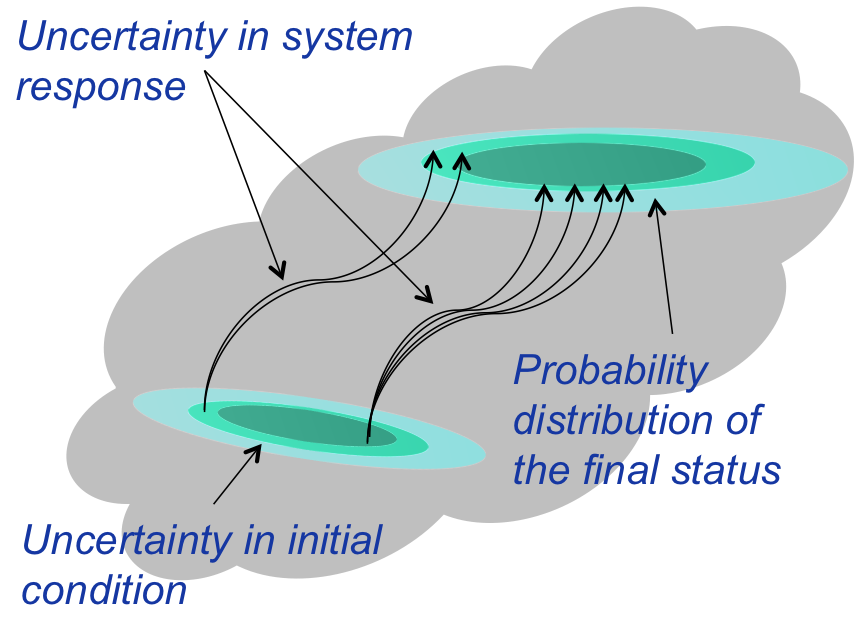
\includegraphics[width=0.7\linewidth]{present/uq}
  \end{figure}
\end{frame}


\begin{frame}{Introduction}{Nomenclature}\vspace{-10pt}
  Consider a generic simulation
  \begin{itemize}
    \item Let $u(Y)$ be a response of interest
    \item Examples:
      \begin{itemize}
        \item peak clad temperature for fuel performance
        \item $k$-eigenvalue for neutronics
        \item power peaking factors for core design
      \end{itemize}
    \item $Y=(y_1,y_2,\ldots,y_N)$ are input parameters
      \begin{itemize}
        \item Material properties
        \item Boundary conditions
        \item Initial conditions
        \item Model tuning parameters
      \end{itemize}
    \item General usage: provided inputs $Y$, obtain response $u(Y)$
  \end{itemize}
\end{frame}



\begin{frame}{Introduction}{Nomenclature}\vspace{-10pt}
  More Definitions
  \vfill
  \begin{itemize}
    \item $u(Y)$ is stochastic response
  \vfill
\item $Y$ is stochastic vector, $Y=(y_1,\ldots,y_N)$
    \item Probability space ($\Omega,\sigma,\rho$)
  \vfill
    \item Each uncertain input $y_n$:
      \begin{itemize}
        \item Probability space ($\Omega_n,\sigma_n,\rho_n$)
        \item Probability Distribution is $\rho_n(Y)$
        \item Realizations $y_n(\omega)$
      \end{itemize}
    \item Full input realization $Y(\omega)$
    \item Response realization $u(Y(\omega))$
  \end{itemize}
  \vfill
\end{frame}


\subsection{Tradition}
\begin{frame}{Introduction}{Traditional Uncertainty Quantification Methods}\vspace{-10pt}
  \begin{columns}
  \begin{column}{0.1\textwidth}
  \end{column}
  \begin{column}{0.45\textwidth}
    Monte Carlo
      \begin{itemize}
        \item Random sampling based on probability
        \item Strong, slow, dimension-agnostic
      \end{itemize}
    Grid
      \begin{itemize}
        \item Nodes equally spaced by probability
        \item Curse of dimensionality
      \end{itemize}
    Latin Hypercube
      \begin{itemize}
        \item Hybrid of MC and Grid
        \item Works for many models
      \end{itemize}
  \end{column}
  \begin{column}{0.45\textwidth}
    \begin{figure}[h!]
      \centering
      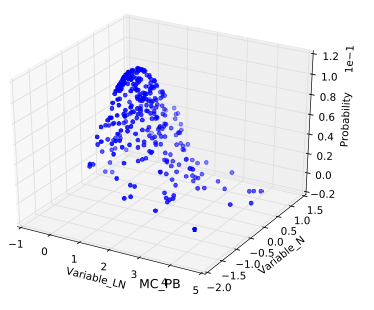
\includegraphics[width=0.4\linewidth]{mc_prob}
    \end{figure}
    \vspace{-10pt}
    \begin{figure}[h!]
      \centering
      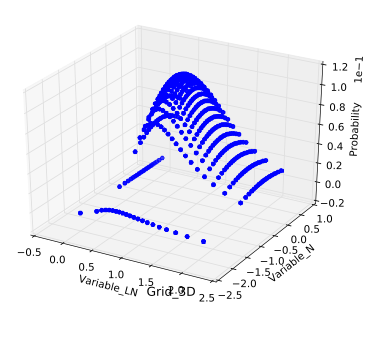
\includegraphics[width=0.4\linewidth]{grid_prob}
    \end{figure}
    \vspace{-10pt}
    \begin{figure}[h!]
      \centering
      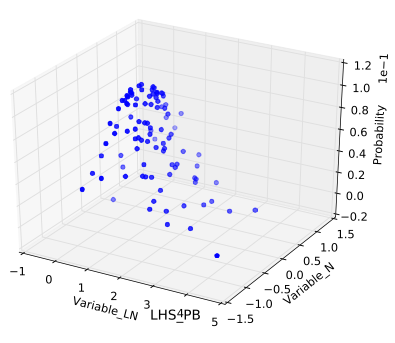
\includegraphics[width=0.4\linewidth]{lhs_prob}
    \end{figure}
  \end{column}
  \end{columns}
\end{frame}


\begin{frame}{Introduction}{Dissertation Objective}\vspace{-20pt}
  \vfill
Objectives of this work
  \vfill
\begin{itemize}
  \item Explore advanced UQ sampling strategies
    \begin{itemize}
      \item Stochastic Collocation for generalized Polynomial Chaos (SCgPC)
      \item High-Dimensional Model Reduction (HDMR)
      \item Adaptive SCgPC
      \item Adaptive HDMR
    \end{itemize}
  \vfill
  \item Advance adaptive methods
  \vfill
  \item Implement all methods in \raven{}
\end{itemize}
  \vfill
\end{frame}





\subsection{Outline}
\begin{frame}{Outline}{Discussion Points}\vspace{-20pt}
  \begin{columns}
  \begin{column}{0.1\textwidth}
  \end{column}
  \begin{column}{0.9\textwidth}
    \setcounter{tocdepth}{1}
    \tableofcontents[hideothersubsections]%,subsectionsonly]
  \end{column}
  \end{columns}
\end{frame}

\AtBeginSubsection[]
{\begin{frame}[shrink=20,noframenumbering]{Outline}\vspace{-20pt}
  \begin{columns}
    \begin{column}{0.1\textwidth}
    \end{column}
    \begin{column}{0.9\textwidth}
      \setcounter{tocdepth}{2}
      \tableofcontents[currentsection,currentsubsection,subsectionstyle=show/shaded/hide]%,hideothersubsections]%hideothersubsections]%,subsectionsonly]
    \end{column}
  \end{columns}
\end{frame}
}






\section{SCgPC}
\subsection{Theory}
\begin{frame}{SCgPC}{Theory}\vspace{-20pt}
  \vfill
  Stochastic Collocation for generalized Polynomial Chaos (SCgPC)
  \vfill
  \begin{enumerate}
    \item Generalized Polynomial Chaos Expansion
  \vfill
    \item Stochastic Collocation
  \vfill
    \item Smolyak Sparse Grids
  \end{enumerate}
  \vfill
\end{frame}

\begin{frame}{SCgPC}{Generalized Polynomial Chaos}\vspace{-20pt}
  \vfill
  Expand model as sum of orthonormal polynomials
  \vfill
  \begin{block}{gPC Expansion}
    \begin{equation*}
    u(Y) \approx G[u](Y) = \sum_{k\in\Lambda(L)} u_k \Phi_k(Y)
    \end{equation*}
  \end{block}
  \vfill
  \begin{itemize}
    \item $\Lambda$: Chosen set of polynomial indices
    \item $k$: Multi-index of polynomial orders e.g. (2,1,3)
    \item $u_k$: Scalar expansions moments
    \item $\Phi_k$: Multidimensional orthonormal polynomials
  \end{itemize}
  \vfill
\end{frame}

\begin{frame}{SCgPC}{gPC: Polynomial Families}\vspace{-20pt}
  \vfill
  \[\Phi_k(Y) = \prod_{n=1}^N \phi^{(n)}_{k_n}(y_n)\]
  \vfill
  Choice of polynomial family depends on distribution of $y_n$
  \vfill
  \begin{table}[h!]
    \centering
    \begin{tabular}{c c}
      Distribution & Polynomial Set \\ \hline
      Uniform & Legendre \\
      Normal & Hermite \\
      Gamma & Laguerre \\
      Beta & Jacobi \\ \hline
      Arbitrary & Legendre
    \end{tabular}
  \end{table}
  \vfill
\end{frame}



\begin{frame}{SCgPC}{gPC: Useful Properties}\vspace{-20pt}
  \begin{block}{gPC Expansion}
    \[u(Y) \approx G[u](Y) = \sum_{k\in\Lambda(L)} u_k \Phi_k(Y)\]
  \end{block}
  \vfill
  \begin{itemize}
    \item Surrogate Model: Polynomials are fast to evaluate
  \vfill
    \item First two moments are very simple
  \end{itemize}
  \vfill
  \begin{equation*}
    \expv{G[u](Y)} = u_{(0,\ldots,0)},\hspace{20pt}\expv{G[u](Y)^2} = \sum_{k\in\Lambda(L)} u_k^2
  \end{equation*}
  \vfill
\end{frame}




\begin{frame}{SCgPC}{gPC: Polynomial Set $\Lambda$}\vspace{-10pt}
  \begin{block}{gPC Expansion}
    \[u(Y) \approx G[u](Y) = \sum_{k\in\Lambda(L)} u_k \Phi_k(Y)\]
  \end{block}
  \vfill
      Choice of polynomial set: $\Lambda(L)$
      \begin{itemize}
        \item Tensor Product
        \item Total Degree
        \item Hyperbolic Cross
      \end{itemize}
      \vfill
      Truncated by limiting order $L$
  \vfill
\end{frame}

\begin{frame}{SCgPC}{gPC: Polynomial Set $\Lambda$}%\vspace{-20pt}
  \vfill
  \centering
  \begin{exampleblock}{Tensor Product Index Set}
    \[\Lambda_\text{TP}(L)=\Big\{k=(k_1,\cdots,k_N): \max_{1\leq n\leq N}k_n\leq L \Big\}\]
  \end{exampleblock}
  \vfill
  Example: $N=2,L=3$
  \vfill
    \begin{table}\centering
      $\Lambda_{TP}(3)=$
      \begin{tabular}{|c c c c|} \hline
        (3,0) & (3,1) & (3,2) & (3,3) \\
        (2,0) & (2,1) & (2,2) & (2,3) \\
        (1,0) & (1,1) & (1,2) & (1,3) \\
        (0,0) & (0,1) & (0,2) & (0,3) \\ \hline
      \end{tabular}
    \end{table}
  \vfill
\end{frame}

\begin{frame}{SCgPC}{gPC: Polynomial Set $\Lambda$}%\vspace{-20pt}
  \vfill
  \centering
  \begin{exampleblock}{Total Degree Index Set}
    \[\Lambda_\text{TD}(L)=\Big\{k=(k_1,\cdots,k_N):\sum_{n=1}^N k_n \leq L \Big\}\]
  \end{exampleblock}
  \vfill
  Example: $N=2,L=3$
  \vfill
    \begin{table}\centering
      $\Lambda_{TD}(3)=$
      \begin{tabular}{|c c c c|} \hline
        (3,0) &       &       &       \\
        (2,0) & (2,1) &       &       \\
        (1,0) & (1,1) & (1,2) &       \\
        (0,0) & (0,1) & (0,2) & (0,3) \\ \hline
      \end{tabular}
    \end{table}
  \vfill
\end{frame}

\begin{frame}{SCgPC}{gPC: Polynomial Set $\Lambda$}%\vspace{-20pt}
  \vfill
  \centering
  \begin{exampleblock}{Hyperbolic Cross Index Set}
    \[\Lambda_\text{HC}(L)=\Big\{k=(k_1,\ldots,k_N):\prod_{n=1}^N\qty(k_n+1) \leq L+1 \Big\}\]
  \end{exampleblock}
  \vfill
  Example: $N=2,L=3$
  \vfill
    \begin{table}\centering
      $\Lambda_{HC}(3)=$
      \begin{tabular}{|c c c c|} \hline
        (3,0) &       &       &       \\
        (2,0) &       &       &       \\
        (1,0) & (1,1) &       &       \\
        (0,0) & (0,1) & (0,2) & (0,3) \\ \hline
      \end{tabular}
    \end{table}
  \vfill
\end{frame}

\begin{frame}{SCgPC}{Adaptive SCgPC}%\vspace{-20pt}
  Choose polynomials to add adaptively
    \begin{figure}[h!]
      \centering
      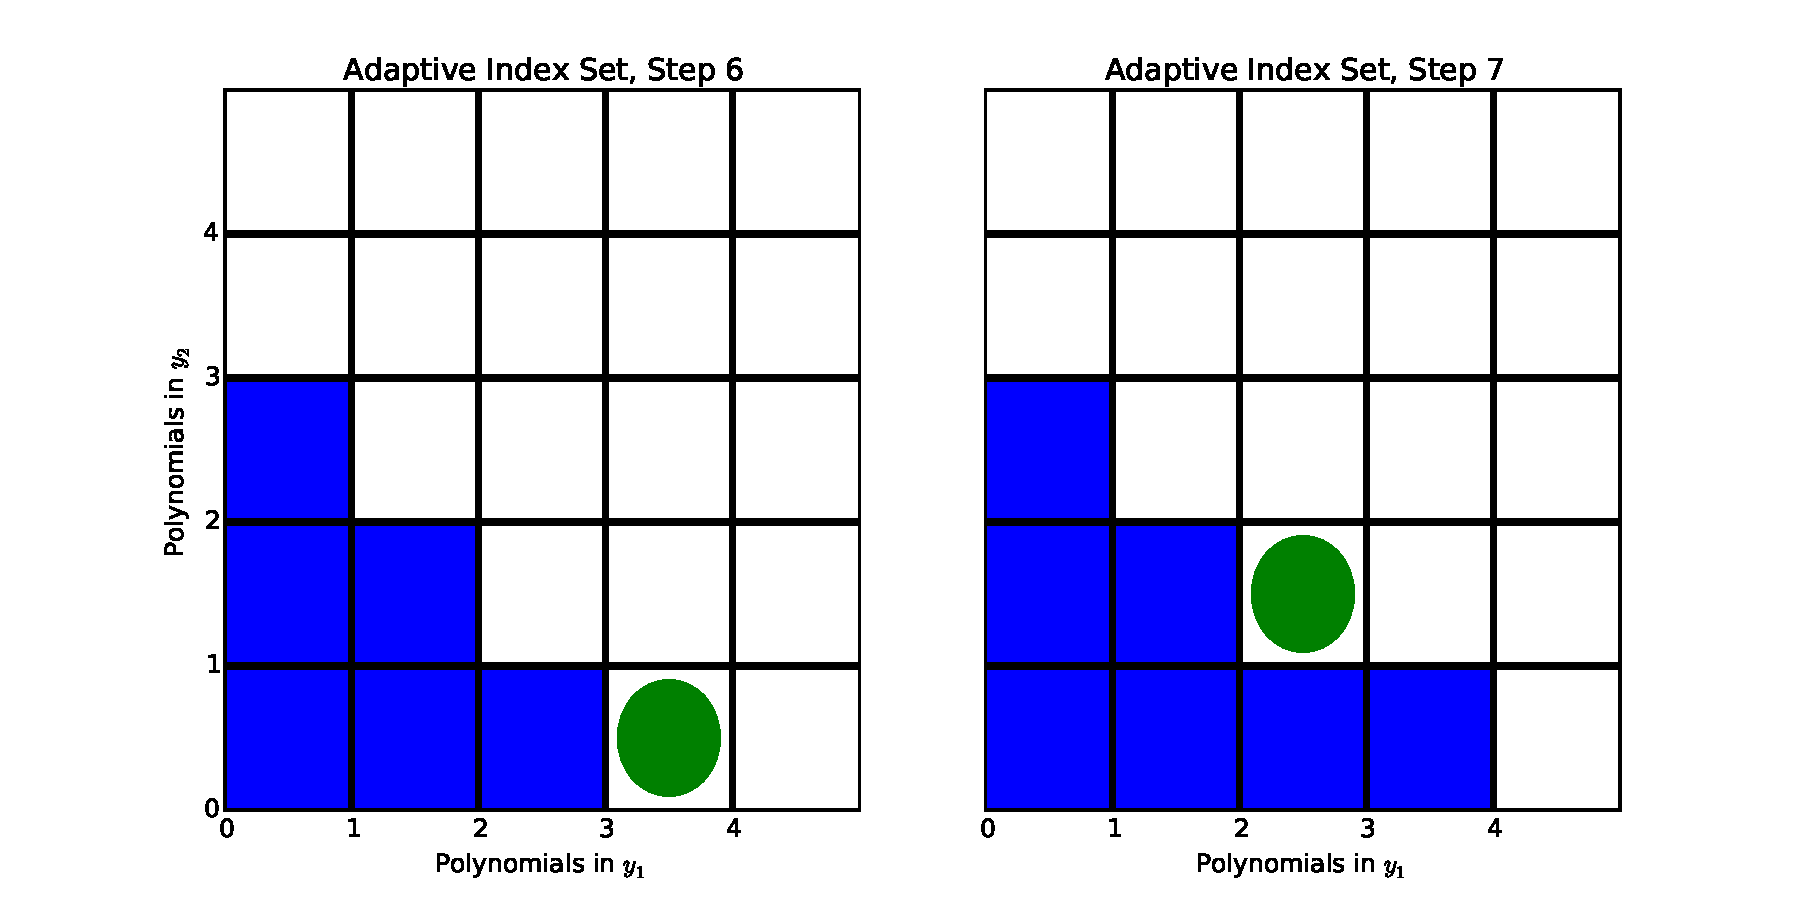
\includegraphics[width=\linewidth]{asc_step}
    \end{figure}
\end{frame}

\begin{frame}{SCgPC}{Adaptive SCgPC}%\vspace{-20pt}
    \begin{figure}[h!]
      \centering
      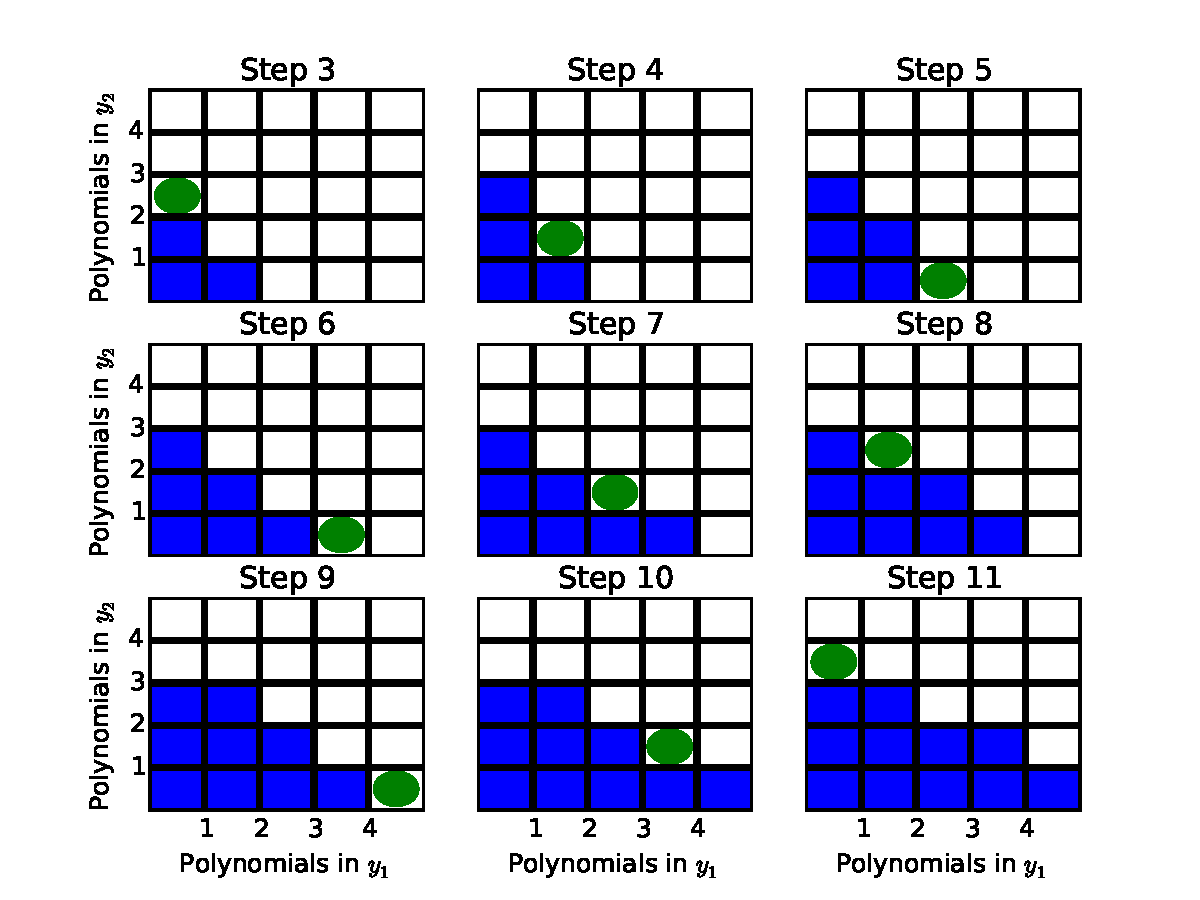
\includegraphics[width=0.8\linewidth]{asc_block}
    \end{figure}
    \vfill
\end{frame}

\begin{frame}{SCgPC}{Adaptive SCgPC}%\vspace{-20pt}
  \vfill
  Predictive Algorithm
  \vfill
  \begin{itemize}
    \item Use variance of previous polynomials to predict
  \vfill
    \item Converge on est. remaining variance
  \vfill
    \item Saves significant evaluations
  \vfill
    \item Assumption: monotonic variance decrease
  \end{itemize}
  \vfill
\end{frame}


\begin{frame}{SCgPC}{gPC: Expansion Moments $u_k$}\vspace{-20pt}
  \vfill
  \begin{block}{gPC Expansion}
    \[u(Y) \approx G[u](Y) = \sum_{k\in\Lambda(L)} u_k \Phi_k(Y)\]
  \end{block}
  \vfill
  Expansion moments $u_k$ given through orthonormality of expansion polynomials
  \vfill
\end{frame}


\begin{frame}{SCgPC}{gPC: Expansion Moments $u_k$}%\vspace{-20pt}
Defining probability-weighted integration and orthonormality,
  \[\int\limits_\Omega (\cdot) dY 
      \equiv 
      \int\limits_{a_1}^{b_1}\rho_1(y_1) \cdots \int\limits_{a_N}^{b_N}\rho_N(y_N) (\cdot)\ dy_1\cdots\ dy_N\]
  \[\int\limits_\Omega \Phi_{j}(Y)\Phi_k(Y) dY = \delta_{j k}\]
  \begin{alertblock}{Expansion Moments}
    \[u_k = \int\limits_\Omega u(Y)\Phi_k(Y) dY\]
  \end{alertblock}
\end{frame}


\begin{frame}{SCgPC}{gPC: Expansion Moments $u_k$}\vspace{-20pt}
  \vfill
  How to integrate
  \begin{alertblock}{Expansion Moments}
    \[u_k = \int\limits_\Omega u(Y)\Phi_k(Y) dY\]
  \end{alertblock}
  \vfill
  \begin{itemize}
    \item Analytic Integration
  \vfill
    \item Monte Carlo sampling
  \vfill
    \item Stochastic Collocation
  \end{itemize}
  \vfill
\end{frame}


\begin{frame}{SCgPC}{Stochastic Collocation}\vspace{-20pt}
  Numerical Integration by Quadrature
  \begin{align*}
    \int\limits_a^b f(y) \rho(y)\ dy &= \sum_{\ell=1}^\infty w_\ell f(y_\ell) \\
      &\approx \sum_{\ell=1}^p w_\ell f(y_\ell) \\
      & \equiv q^{(p)}\qty[f(y)]
  \end{align*}
  \vfill
\end{frame}

\begin{frame}{SCgPC}{Stochastic Collocation}\vspace{-20pt}
  Gauss quadrature
  \begin{itemize}
    \item Exact for polynomials order $2p-1$
    \item Several quadratures for several weights
    \item Correspond to expansion polynomials
  \end{itemize}
  \begin{table}[h!]
    \centering
    \begin{tabular}{c c c}
      Distribution & Polynomial Set & Quadrature\\ \hline
      Uniform & Legendre & Legendre\\
      Normal & Hermite & Hermite\\
      Gamma & Laguerre & Laguerre\\
      Beta & Jacobi & Jacobi
    \end{tabular}
  \end{table}
\end{frame}


\begin{frame}{SCgPC}{Stochastic Collocation}\vspace{-20pt}
  \begin{alertblock}{Expansion Moments}
    \[u_k = \int\limits_\Omega u(Y)\Phi_k(Y) dY\]
  \end{alertblock}
  Integration Order and Quadrature Order
  Order of $u(Y)\Phi_k(Y)$
  \begin{itemize}
    \item Order of $\Phi_k(Y)$ is $k$
    \item Order of $u(Y)$ is unknown; assume $\mathcal{O}(G[u](Y))$
    \item Total order is $2k$ $\to$ $p_n = k_n+\frac{1}{2}$
  \end{itemize}
  Number of points should be $k_n+1$ for each dimension $n$
\end{frame}


\begin{frame}{SCgPC}{Stochastic Collocation}\vspace{-20pt}
  Multidimensional Numerical Integrals
  \vfill
  Basic choice: tensor combination
  \begin{columns}
    \begin{column}{0.6\textwidth}
      \begin{equation*}
        \int\limits_{a_1}^{b_1}\int\limits_{a_2}^{b_2} f(Y) \rho(Y)\ dy_2\ dy_1 \approx Q^{(\vec p)}\qty[f(Y)]
      \end{equation*}
      \begin{align*}
        Q^{(\vec p)} &= q^{(p_1)} \otimes q^{(p_2)} \\
          &= \bigotimes_{n=1}^N q^{(p_n)}
      \end{align*}
    \end{column}
    \begin{column}{0.4\textwidth}
    \begin{figure}[h!]
      \centering
      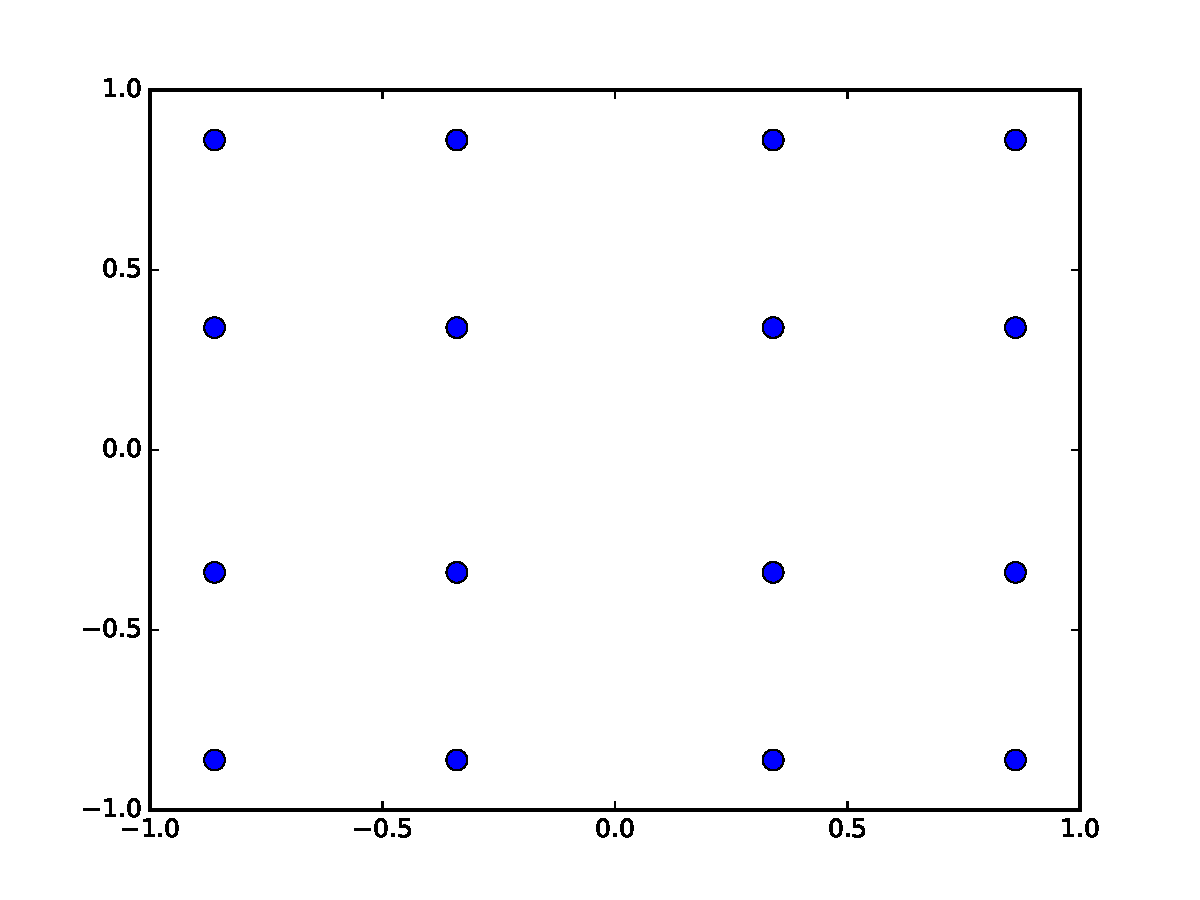
\includegraphics[width=\linewidth]{tensor_quad}
    \end{figure}
    \end{column}
  \end{columns}
\end{frame}

\begin{frame}{SCgPC}{Smolyak Sparse Grid}%\vspace{-20pt}
  Tensor quadrature can be wasteful
    \begin{table}\centering
      $\Lambda_{HC}(3)=$
      \begin{tabular}{|c c c c|} \hline
        \color{red}{(3,0)} &       &       &       \\
        (2,0) &       &       &       \\
        (1,0) & \color{red}{(1,1)} &       &       \\
        (0,0) & (0,1) & (0,2) & \color{red}{(0,3)} \\ \hline
      \end{tabular}
    \end{table}
    \begin{columns}
      \begin{column}{0.6\textwidth}
        Need fewer knots and weights
        \begin{itemize}
          \item 4th order in $y_1$
          \item 4th order in $y_2$
          \item 2nd $\cross$ 2nd in ($y_1,y_2$)
        \end{itemize}
        Requires 12 instead of 16 points
      \end{column}
      \begin{column}{0.4\textwidth}
        \begin{figure}[h!]
          \centering
          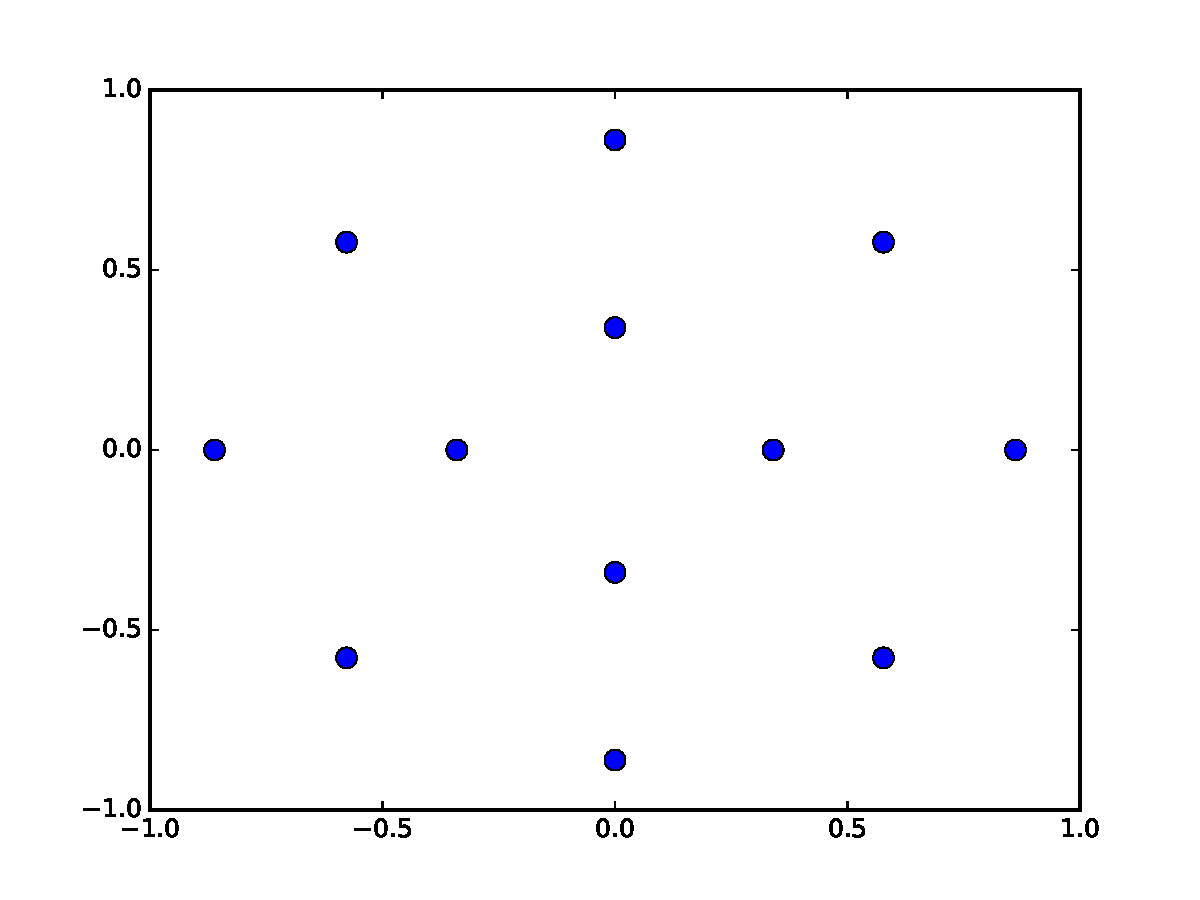
\includegraphics[width=\linewidth]{smolyak_quad}
        \end{figure}
      \end{column}
    \end{columns}
\end{frame}


\begin{frame}{SCgPC}{Smolyak Sparse Grid}%\vspace{-20pt}
  Smolyak Sparse Grid Quadrature
  \begin{equation*}
    S^{(\vec p)}_{\Lambda,N}[(\cdot)] = \sum_{k\in\Lambda(L)} c(k)\bigotimes_{n=1}^N
    q^{(p_n)}_n[(\cdot)]
  \end{equation*}
  \begin{equation*}
    c(k) = \sum_{\substack{j=\{0,1\}^N,\\k+j\in\Lambda(L)}} (-1)^{|j|_1},
  \end{equation*}
\end{frame}


\begin{frame}{SCgPC}{Smolyak Sparse Grid}\vspace{-20pt}
  \begin{alertblock}{Expansion Moments}
    \[u_k = \int\limits_\Omega u(Y)\Phi_k(Y) dY\]
  \end{alertblock}
  Calculate using Smolyak sparse grid
  \begin{equation*}
    u_k \approx S^{(\vec p)}_{\Lambda,N}[u(Y)\Phi_k(Y)]
  \end{equation*}
  \begin{block}{gPC Expansion}
    \[u(Y) \approx G[u](Y) = \sum_{k\in\Lambda(L)} u_k \Phi_k(Y)\]
  \end{block}
\end{frame}



\subsection{Results}

\begin{frame}{SCgPC Results}{Introduction}\vspace{-20pt}
  \vfill
Performed analysis on several analytic models
  \vfill
Considered impact of
  \vfill
\begin{itemize}
  \item Changing regularity
  \vfill
  \item Changing dimensionality
  \vfill
  \item Different polynomial representations
\end{itemize}
  \vfill
  Consider TP, TD, HC, and Adaptive SCgPC
  \vfill
\end{frame}

\begin{frame}{SCgPC Results}{Models}\vspace{-20pt}
  \vfill
  Analytic models used
  \vfill
  \begin{columns}
    \begin{column}{0.5\textwidth}
  \vfill
      \begin{itemize}
        \item Tensor Monomials
  \vfill
        \item Sudret Polynomial
  \vfill
        \item Attenuation
      \end{itemize}
  \vfill
    \end{column}
    \begin{column}{0.5\textwidth}
  \vfill
      \begin{itemize}
        \item Gauss Peak
  \vfill
        \item Ishigami
  \vfill
        \item Sobol G-Function
      \end{itemize}
  \vfill
    \end{column}
  \end{columns}
  \vfill
\end{frame}


\subsubsection{Tensor Monomials}
\begin{frame}{SCgPC Results}{Tensor Monomials}\vspace{-20pt}
  \begin{columns}
    \begin{column}{0.6\textwidth}
      \begin{block}{Tensor Monomials}
        \[u(Y) = \prod_{n=1}^N (y_n+1)\]
      \end{block}
    \end{column}
    \begin{column}{0.4\textwidth}
        \begin{figure}[h!]
          \centering
          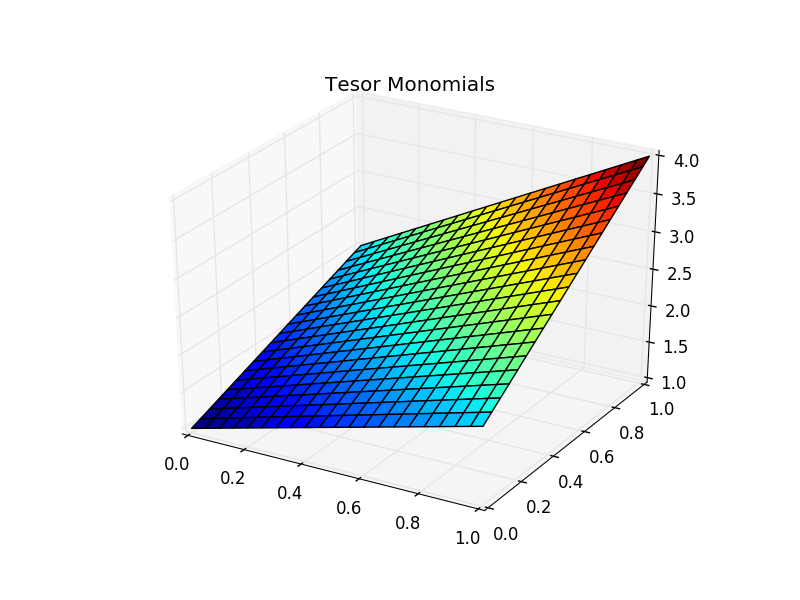
\includegraphics[width=\linewidth]{anlmodels/tensor_monom}
        \end{figure}
    \end{column}
  \end{columns}
  \begin{itemize}
    \item Linear response
    \item All polynomial combinations
  \end{itemize}
\end{frame}
\begin{frame}{SCgPC Results}{Tensor Monomials, $N=3$}\vspace{-20pt}
 \begin{columns}
   \begin{column}{0.5\textwidth}
        \begin{figure}[h!]
          \centering
          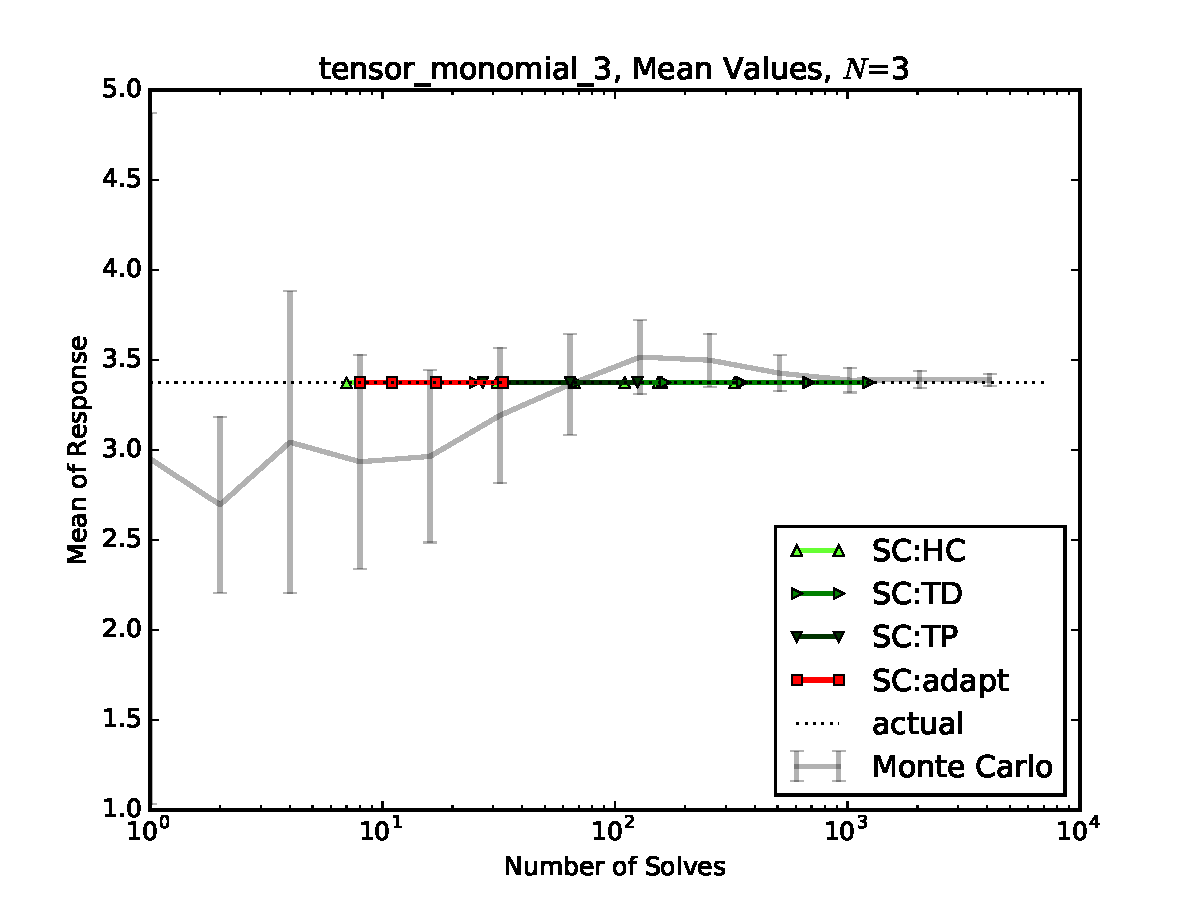
\includegraphics[width=0.8\linewidth]{anlmodels/tensor_monomial_3_mean_vals_nohdmr}
        \end{figure}
        \vspace{-20pt}
        \begin{figure}[h!]
          \centering
          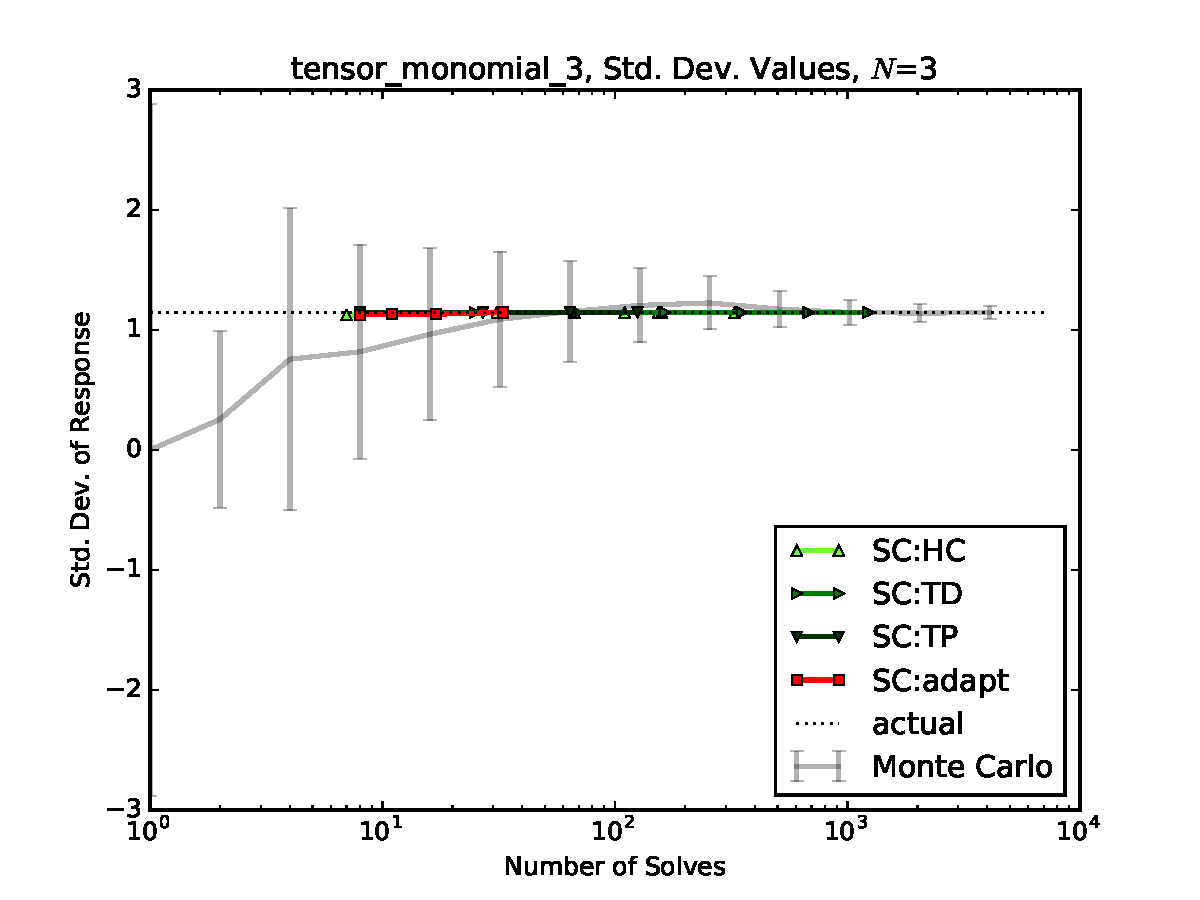
\includegraphics[width=0.8\linewidth]{anlmodels/tensor_monomial_3_var_vals_nohdmr}
        \end{figure}
   \end{column}
   \begin{column}{0.5\textwidth}
        \begin{figure}[h!]
          \centering
          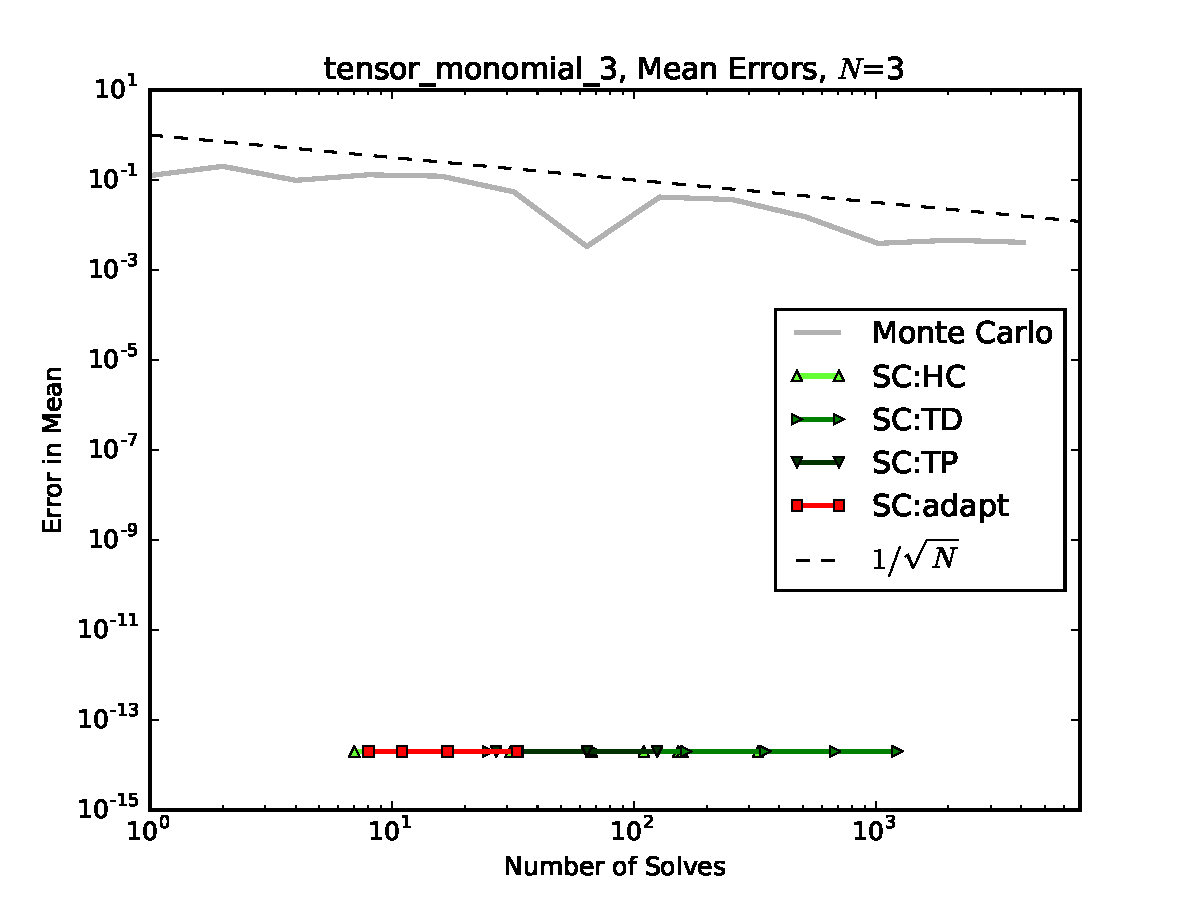
\includegraphics[width=0.8\linewidth]{anlmodels/tensor_monomial_3_mean_errs_nohdmr}
        \end{figure}
        \vspace{-20pt}
        \begin{figure}[h!]
          \centering
          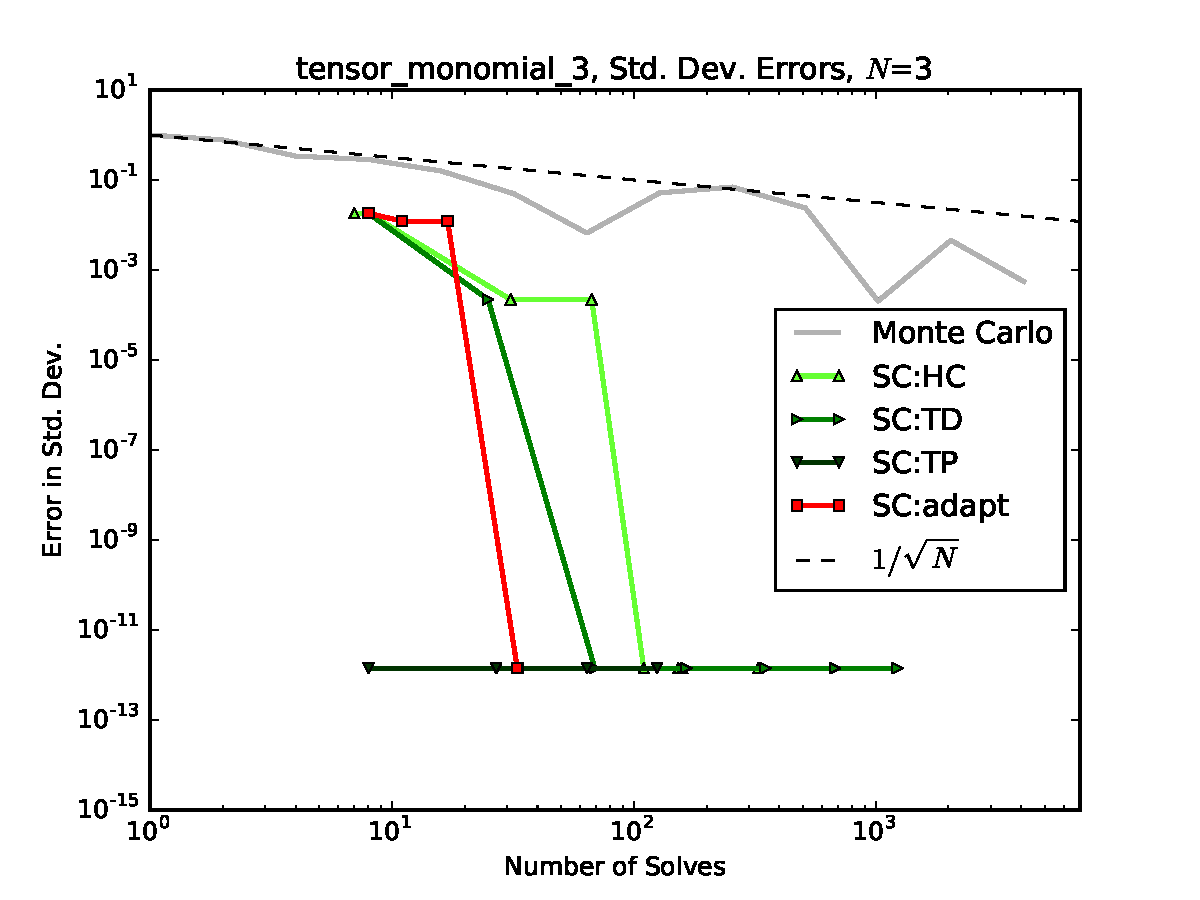
\includegraphics[width=0.8\linewidth]{anlmodels/tensor_monomial_3_variance_errs_nohdmr}
        \end{figure}
   \end{column}
 \end{columns}
\end{frame}
\begin{frame}{SCgPC Results}{Tensor Monomials, $N=5$}\vspace{-20pt}
 \begin{columns}
   \begin{column}{0.5\textwidth}
        \begin{figure}[h!]
          \centering
          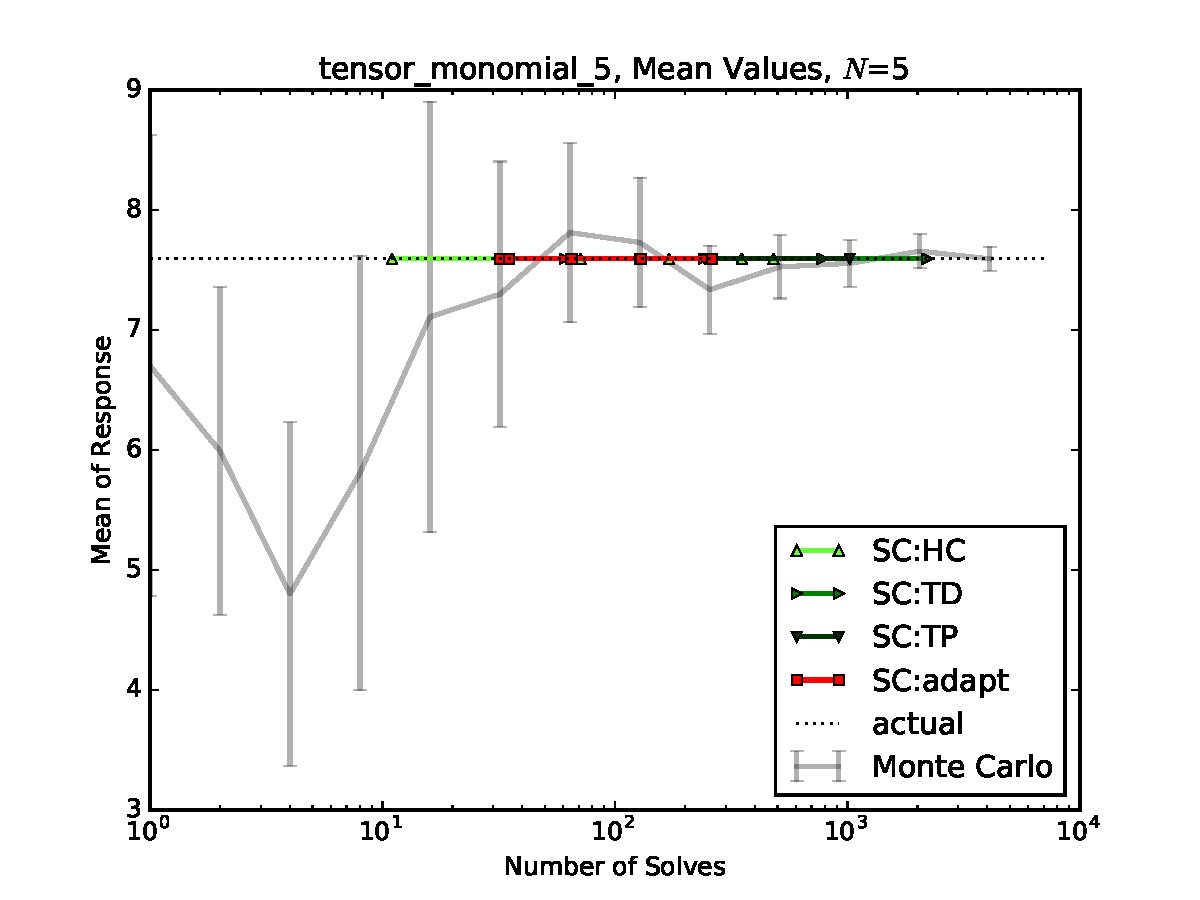
\includegraphics[width=0.8\linewidth]{anlmodels/tensor_monomial_5_mean_vals_nohdmr}
        \end{figure}
        \vspace{-20pt}
        \begin{figure}[h!]
          \centering
          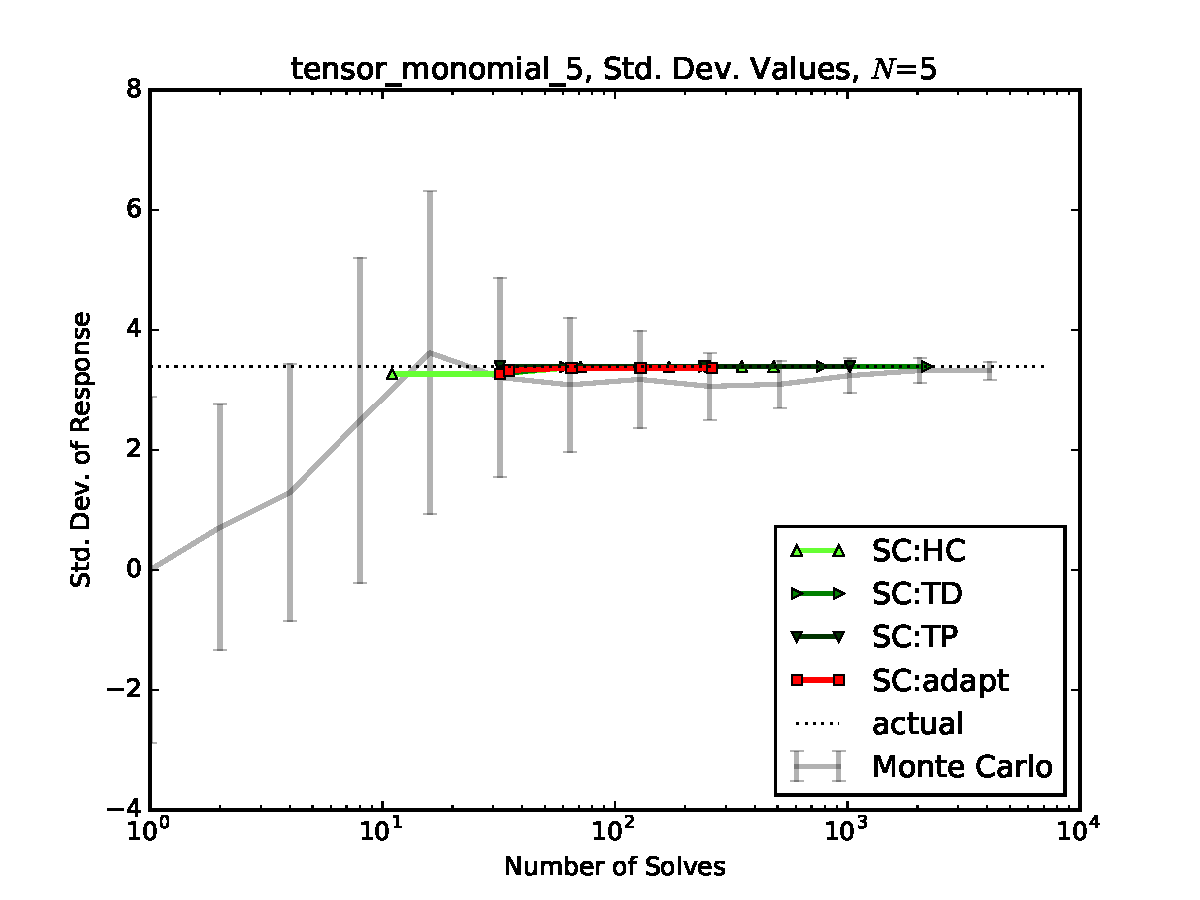
\includegraphics[width=0.8\linewidth]{anlmodels/tensor_monomial_5_var_vals_nohdmr}
        \end{figure}
   \end{column}
   \begin{column}{0.5\textwidth}
        \begin{figure}[h!]
          \centering
          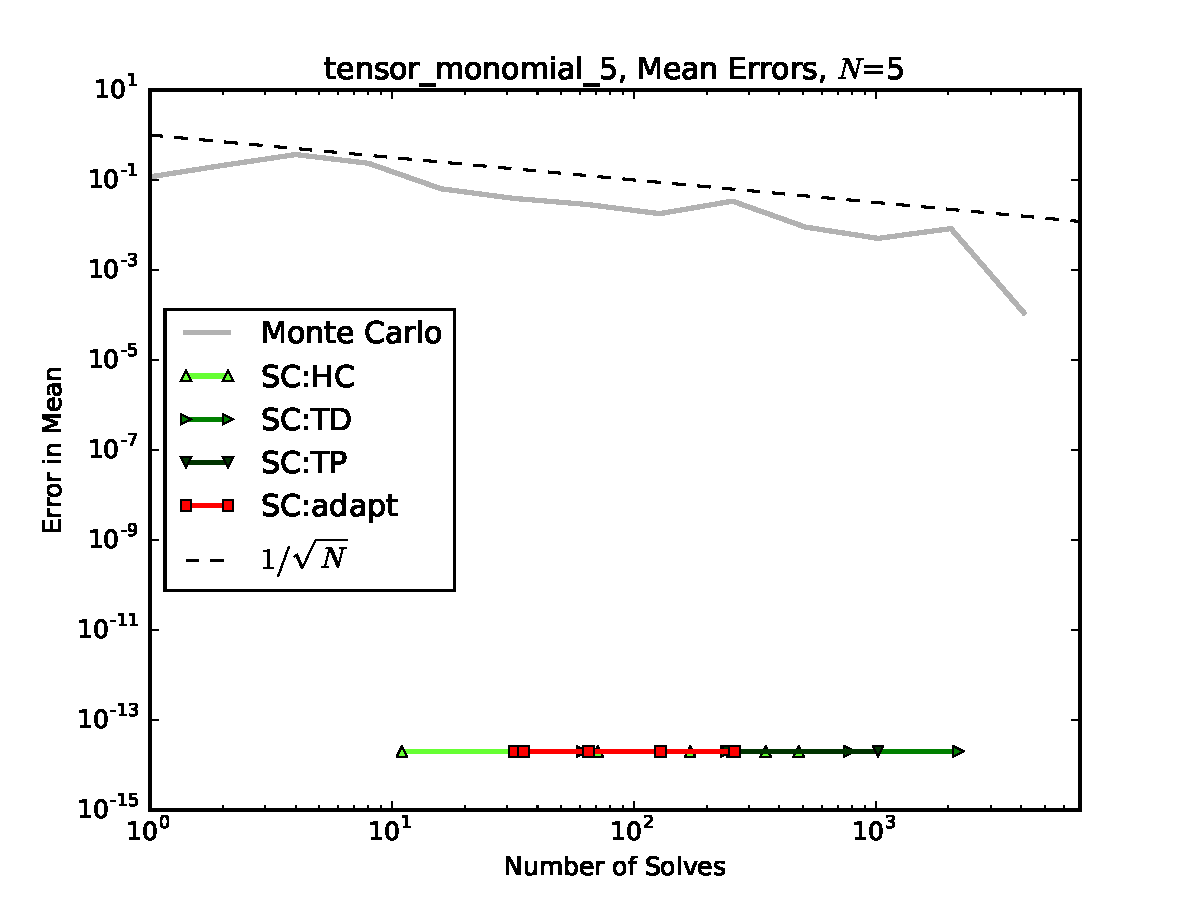
\includegraphics[width=0.8\linewidth]{anlmodels/tensor_monomial_5_mean_errs_nohdmr}
        \end{figure}
        \vspace{-20pt}
        \begin{figure}[h!]
          \centering
          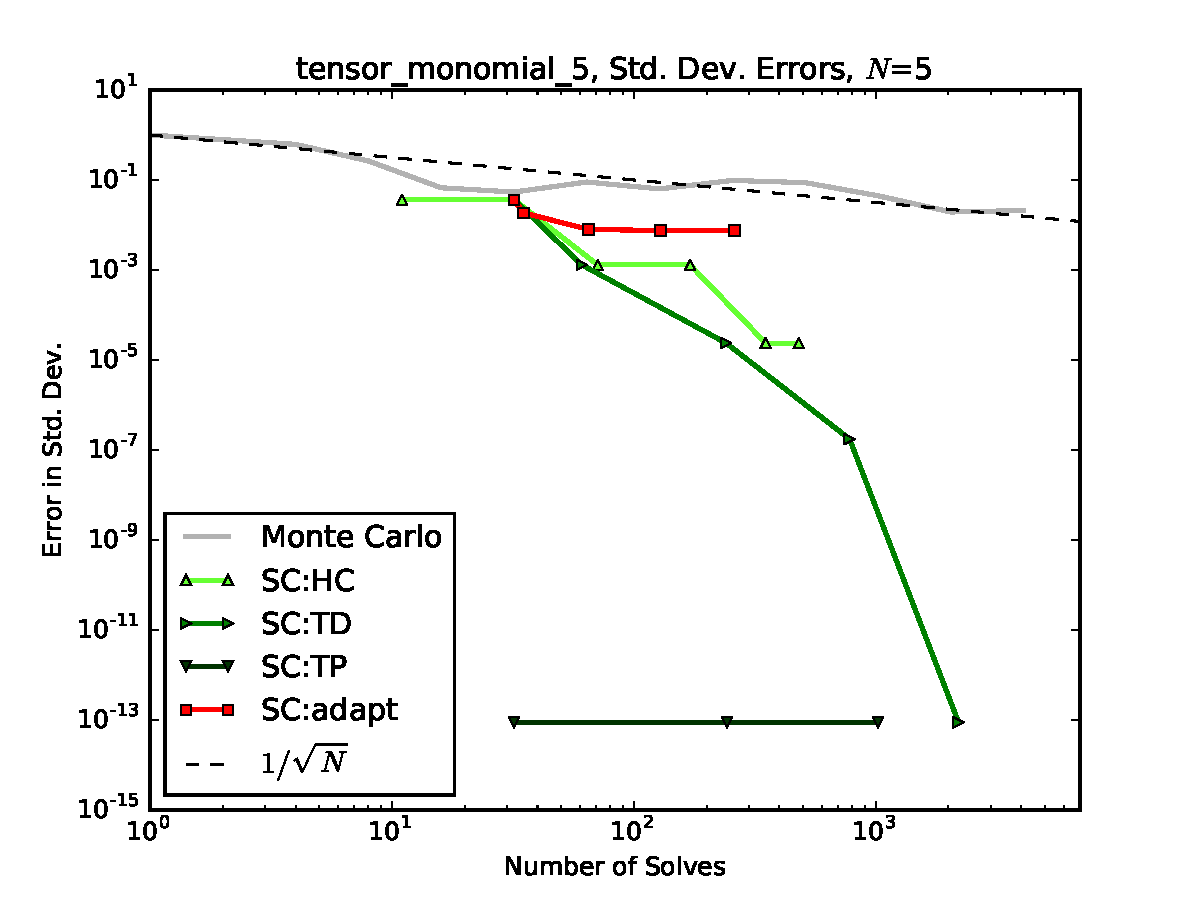
\includegraphics[width=0.8\linewidth]{anlmodels/tensor_monomial_5_variance_errs_nohdmr}
        \end{figure}
   \end{column}
 \end{columns}
\end{frame}
\begin{frame}{SCgPC Results}{Tensor Monomials, $N=10$}\vspace{-20pt}
 \begin{columns}
   \begin{column}{0.5\textwidth}
        \begin{figure}[h!]
          \centering
          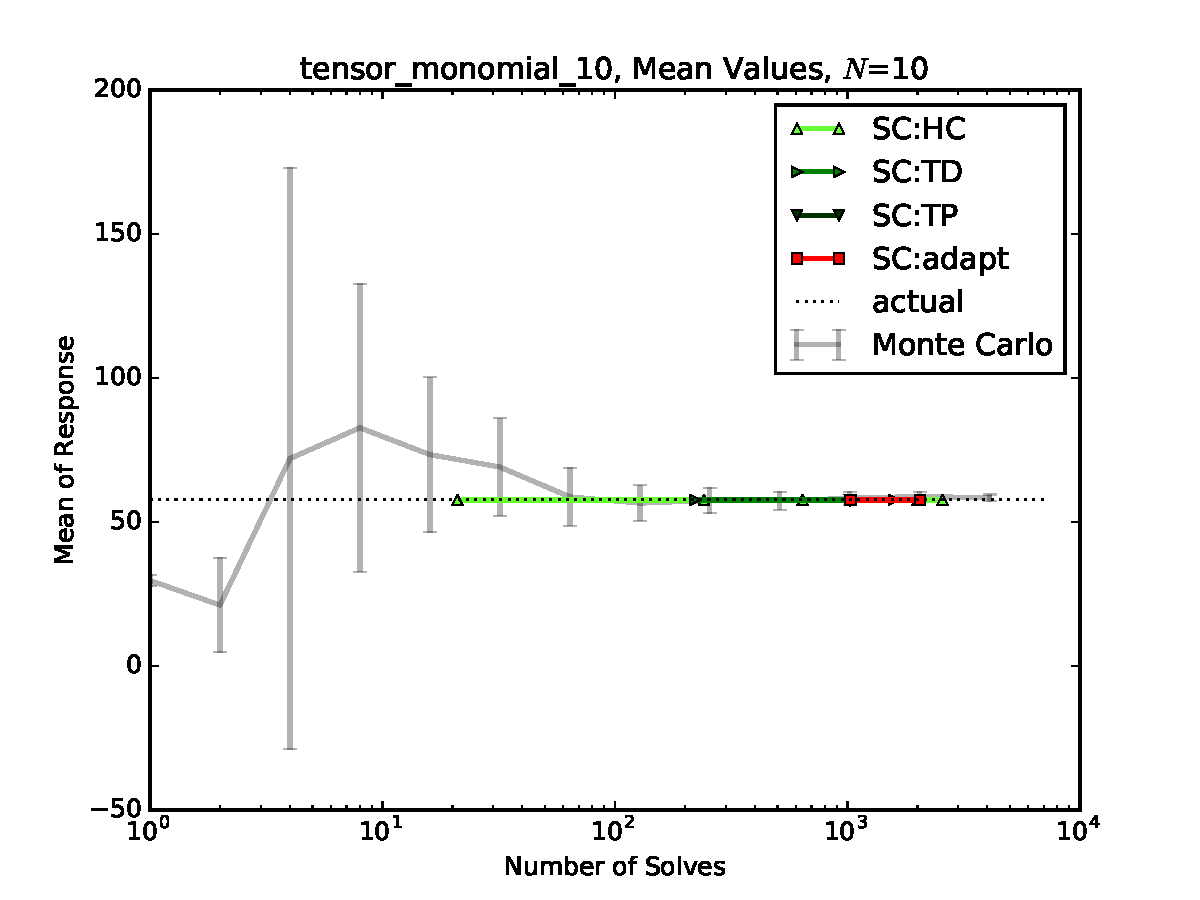
\includegraphics[width=0.8\linewidth]{anlmodels/tensor_monomial_10_mean_vals_nohdmr}
        \end{figure}
        \vspace{-20pt}
        \begin{figure}[h!]
          \centering
          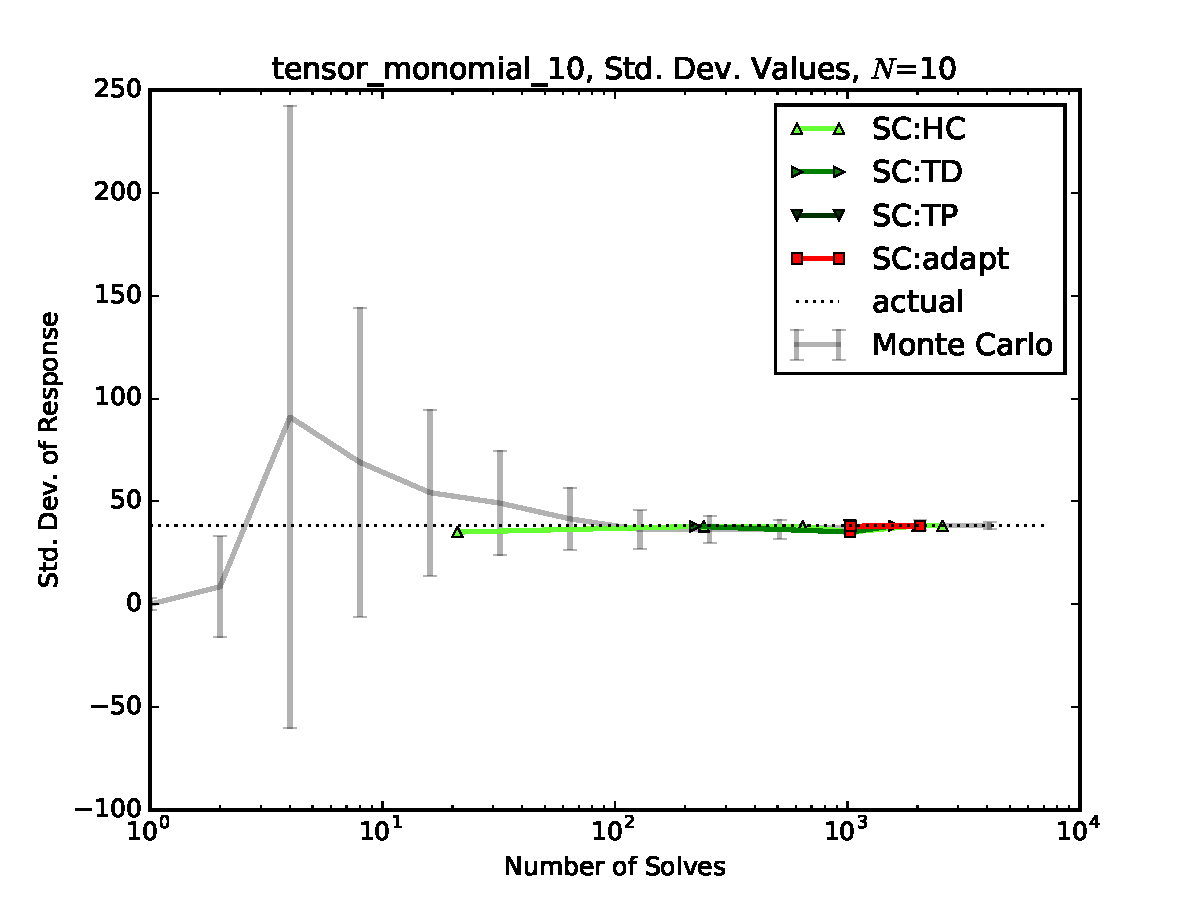
\includegraphics[width=0.8\linewidth]{anlmodels/tensor_monomial_10_var_vals_nohdmr}
        \end{figure}
   \end{column}
   \begin{column}{0.5\textwidth}
        \begin{figure}[h!]
          \centering
          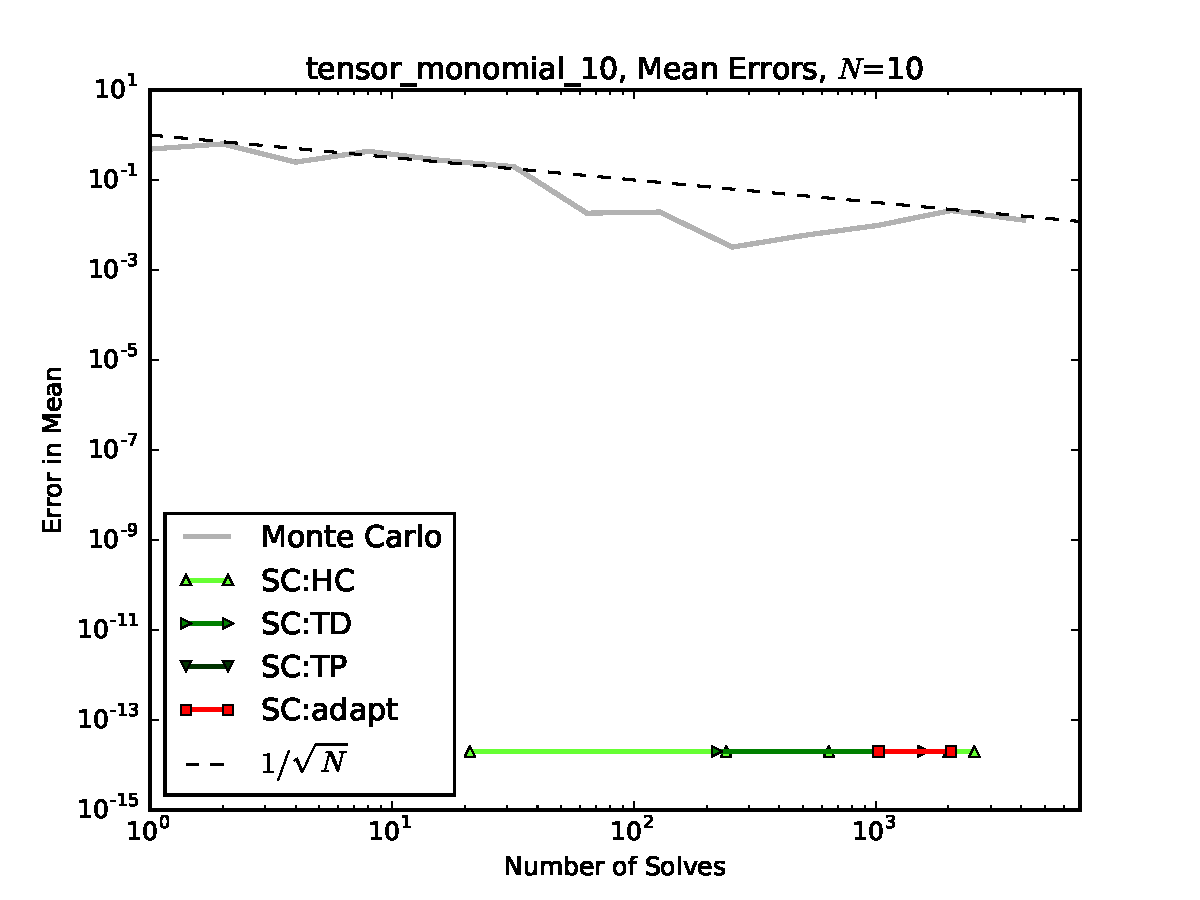
\includegraphics[width=0.8\linewidth]{anlmodels/tensor_monomial_10_mean_errs_nohdmr}
        \end{figure}
        \vspace{-20pt}
        \begin{figure}[h!]
          \centering
          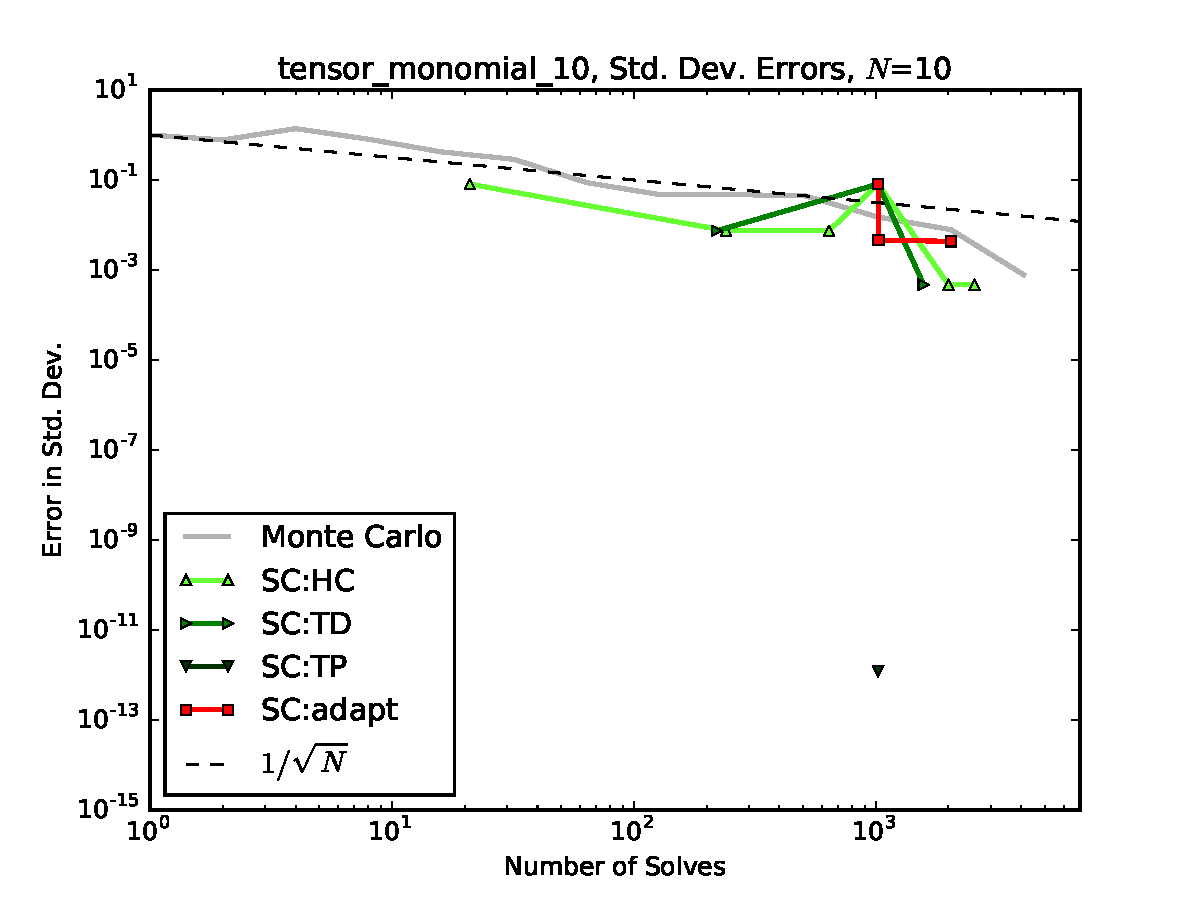
\includegraphics[width=0.8\linewidth]{anlmodels/tensor_monomial_10_variance_errs_nohdmr}
        \end{figure}
   \end{column}
 \end{columns}
\end{frame}



\subsubsection{Sudret Polynomial}
\begin{frame}{SCgPC Results}{Sudret Polynomials}\vspace{-20pt}
  \begin{columns}
    \begin{column}{0.6\textwidth}
      \begin{block}{Sudret Polynomials}
        \[u(Y) = \frac{1}{2^N}\prod_{n=1}^N (3y_n^2+1)\]
      \end{block}
    \end{column}
    \begin{column}{0.4\textwidth}
        \begin{figure}[h!]
          \centering
          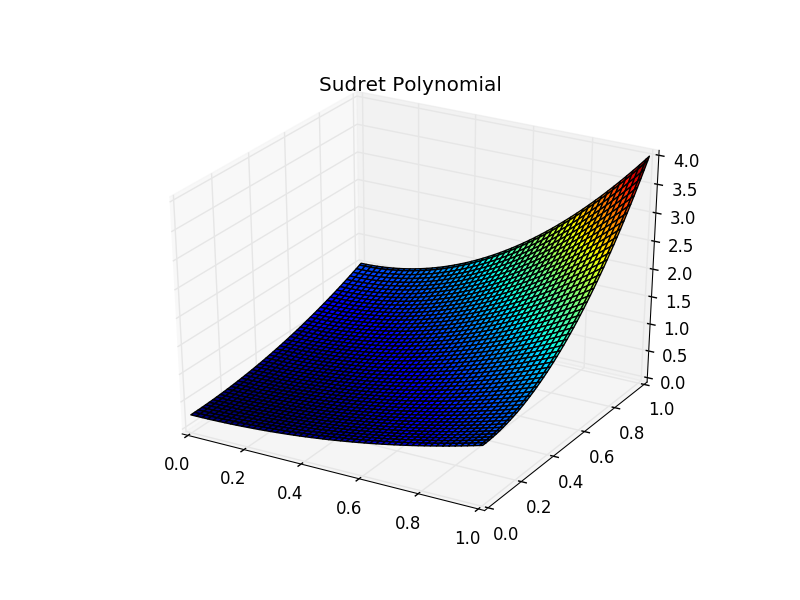
\includegraphics[width=\linewidth]{anlmodels/sudret}
        \end{figure}
    \end{column}
  \end{columns}
  \begin{itemize}
    \item Exclusively second-order interactions
    \item All second-order polynomial combinations
  \end{itemize}
\end{frame}
\begin{frame}{SCgPC Results}{Sudret Polynomials, $N=3$}\vspace{-20pt}
 \begin{columns}
   \begin{column}{0.5\textwidth}
        \begin{figure}[h!]
          \centering
          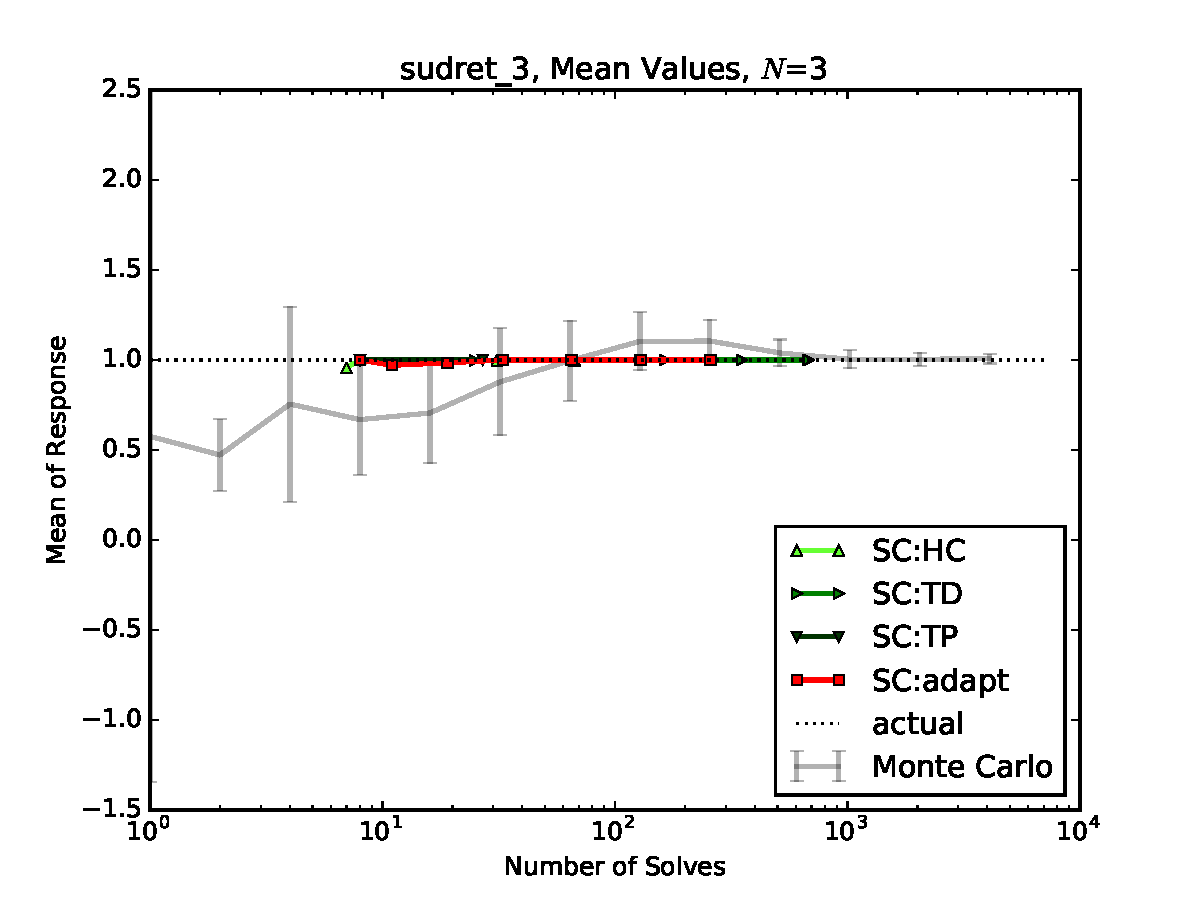
\includegraphics[width=0.8\linewidth]{anlmodels/sudret_3_mean_vals_nohdmr}
        \end{figure}
        \vspace{-20pt}
        \begin{figure}[h!]
          \centering
          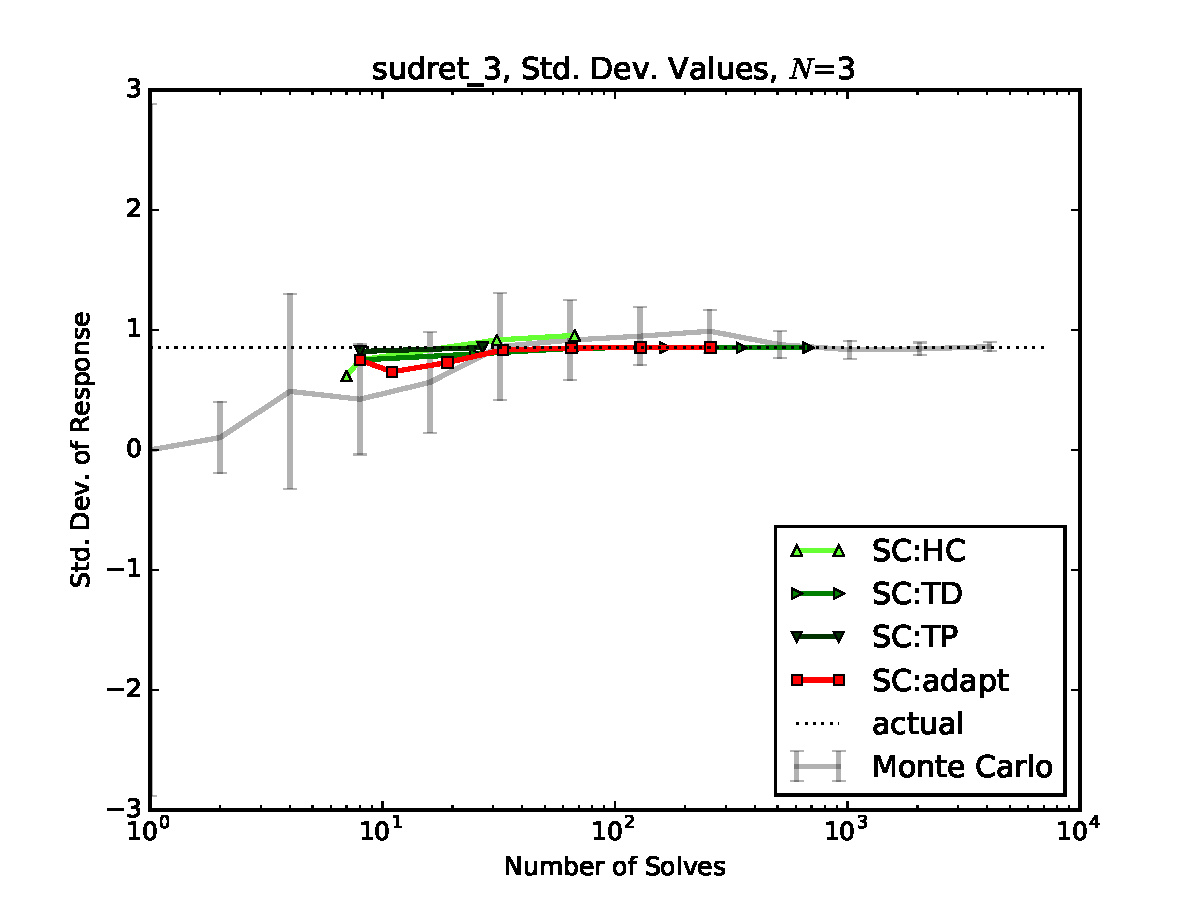
\includegraphics[width=0.8\linewidth]{anlmodels/sudret_3_var_vals_nohdmr}
        \end{figure}
   \end{column}
   \begin{column}{0.5\textwidth}
        \begin{figure}[h!]
          \centering
          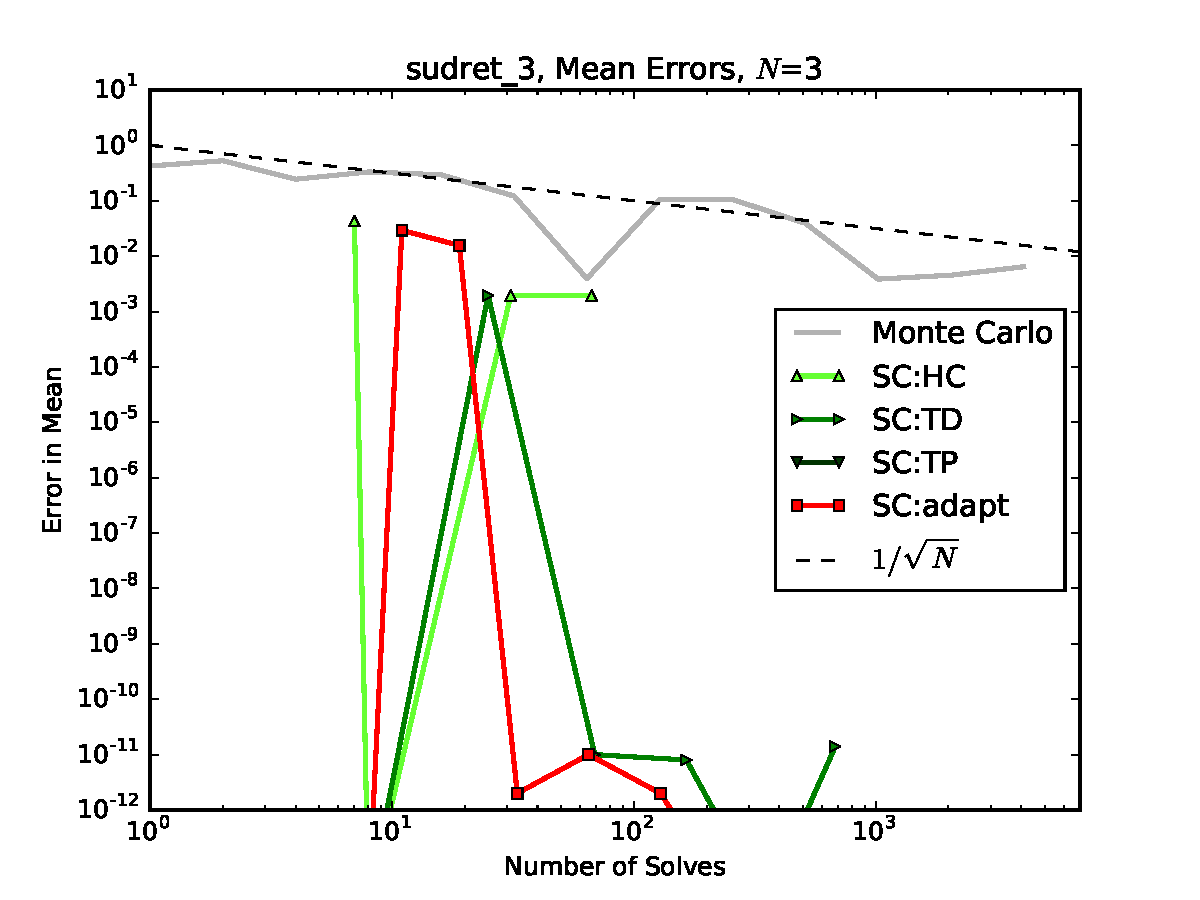
\includegraphics[width=0.8\linewidth]{anlmodels/sudret_3_mean_errs_nohdmr}
        \end{figure}
        \vspace{-20pt}
        \begin{figure}[h!]
          \centering
          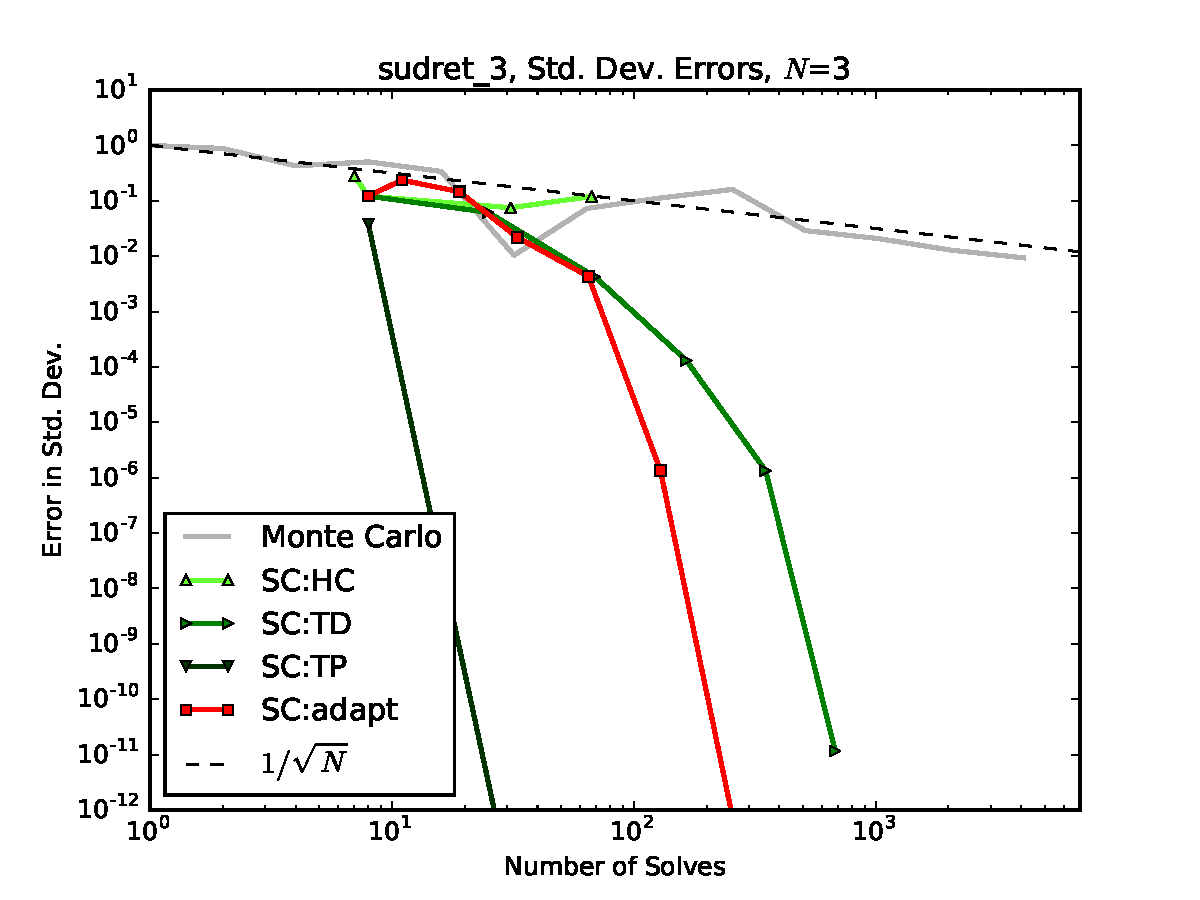
\includegraphics[width=0.8\linewidth]{anlmodels/sudret_3_variance_errs_nohdmr}
        \end{figure}
   \end{column}
 \end{columns}
\end{frame}
\begin{frame}{SCgPC Results}{Sudret Polynomials, $N=5$}\vspace{-20pt}
 \begin{columns}
   \begin{column}{0.5\textwidth}
        \begin{figure}[h!]
          \centering
          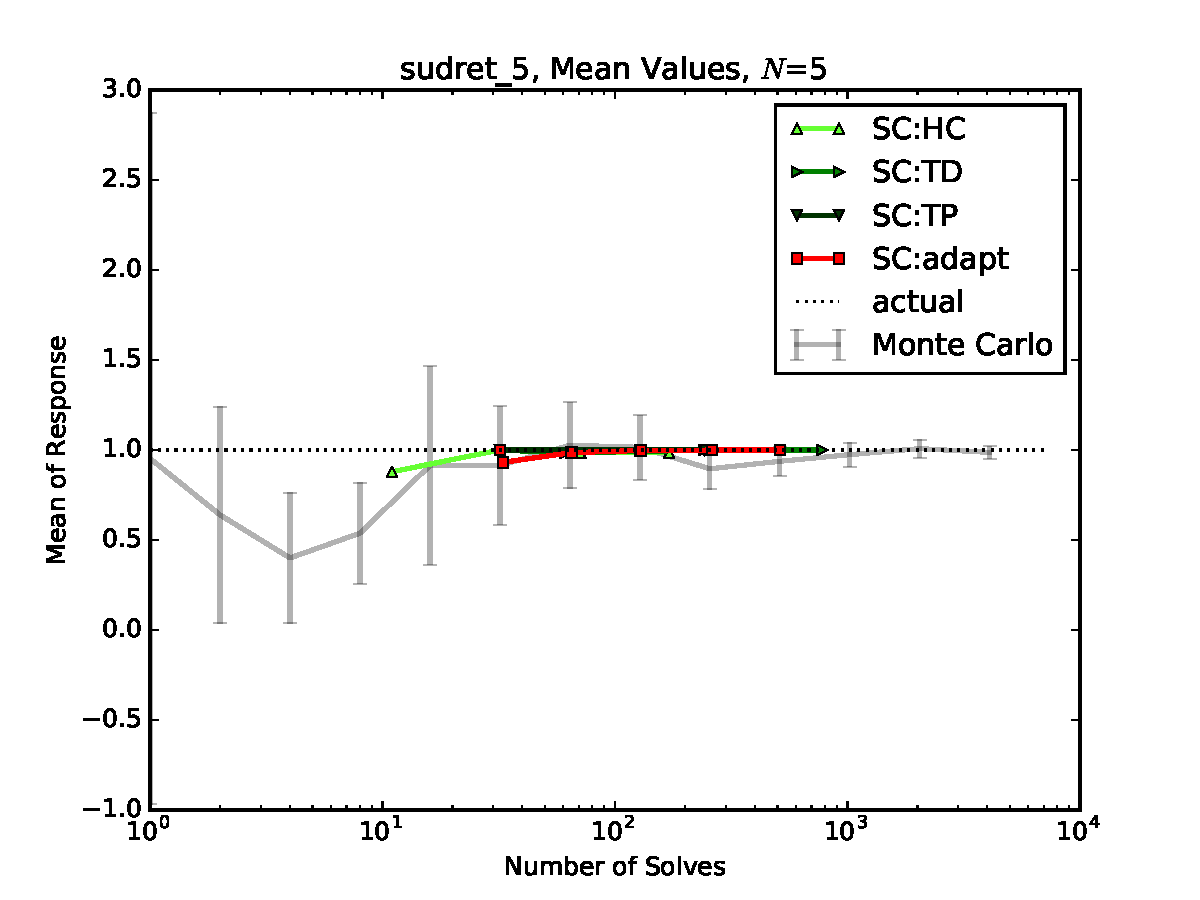
\includegraphics[width=0.8\linewidth]{anlmodels/sudret_5_mean_vals_nohdmr}
        \end{figure}
        \vspace{-20pt}
        \begin{figure}[h!]
          \centering
          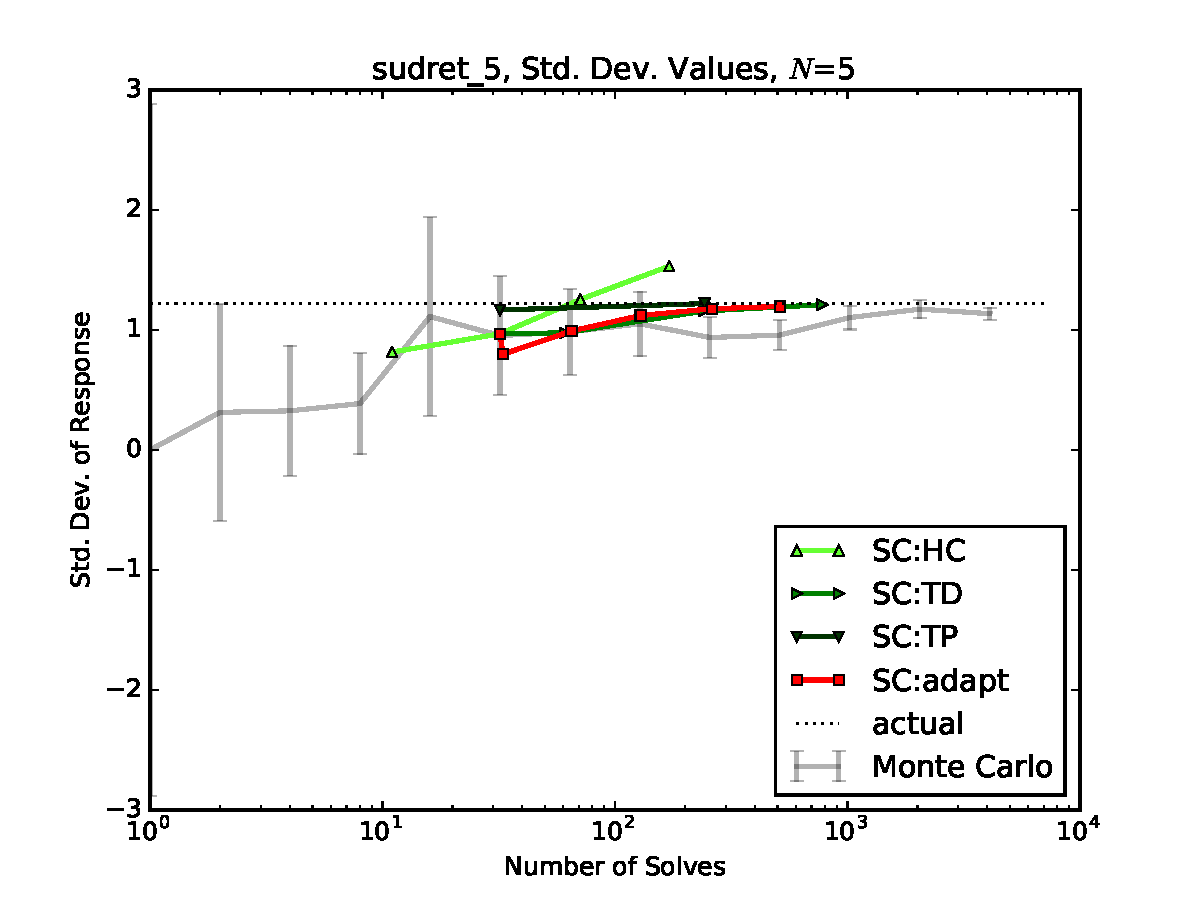
\includegraphics[width=0.8\linewidth]{anlmodels/sudret_5_var_vals_nohdmr}
        \end{figure}
   \end{column}
   \begin{column}{0.5\textwidth}
        \begin{figure}[h!]
          \centering
          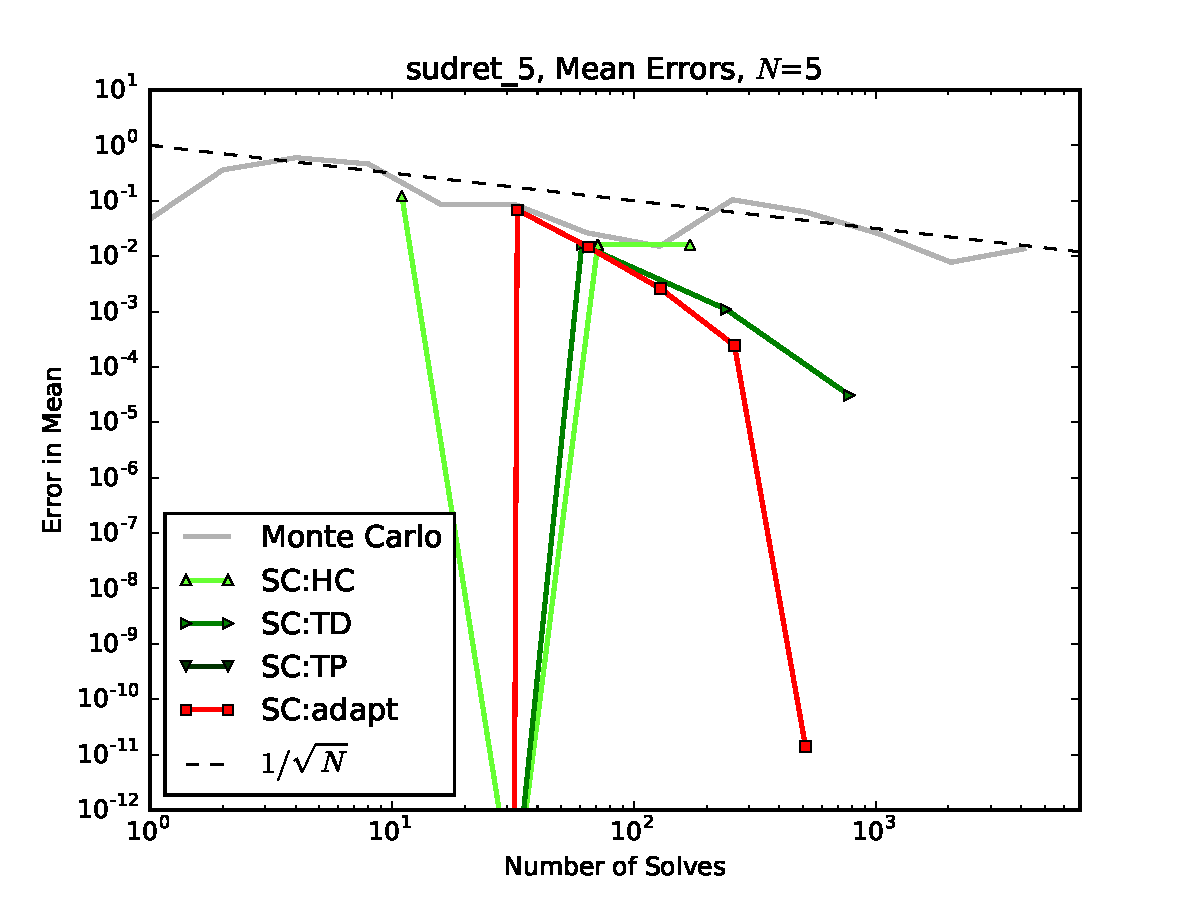
\includegraphics[width=0.8\linewidth]{anlmodels/sudret_5_mean_errs_nohdmr}
        \end{figure}
        \vspace{-20pt}
        \begin{figure}[h!]
          \centering
          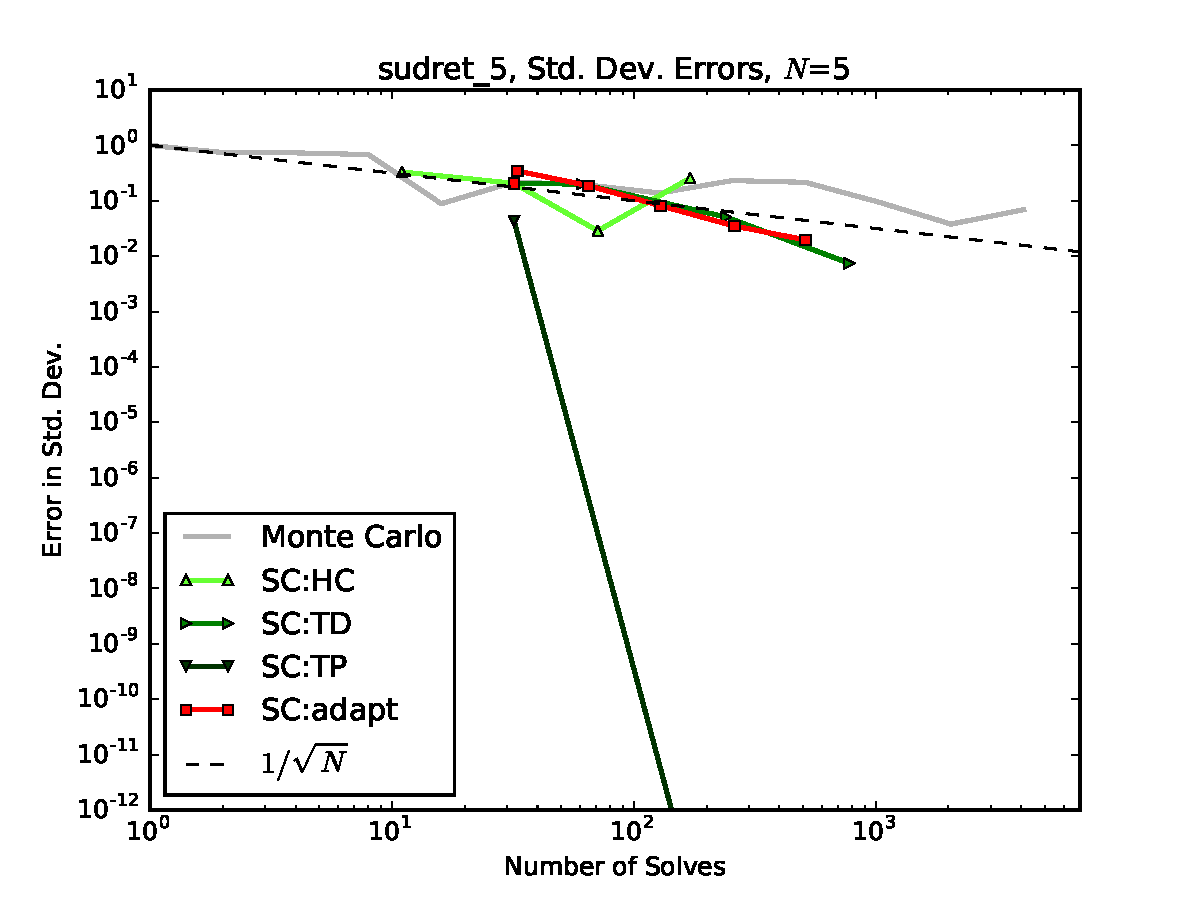
\includegraphics[width=0.8\linewidth]{anlmodels/sudret_5_variance_errs_nohdmr}
        \end{figure}
   \end{column}
 \end{columns}
\end{frame}


\subsubsection{Attenuation}
\begin{frame}{SCgPC Results}{Attenuation}\vspace{-20pt}
  \begin{columns}
    \begin{column}{0.6\textwidth}
      \begin{block}{Attenuation}
        \[u(Y) = \prod_{n=1}^N \exp(-y_n/N)\]
      \end{block}
    \end{column}
    \begin{column}{0.4\textwidth}
        \begin{figure}[h!]
          \centering
          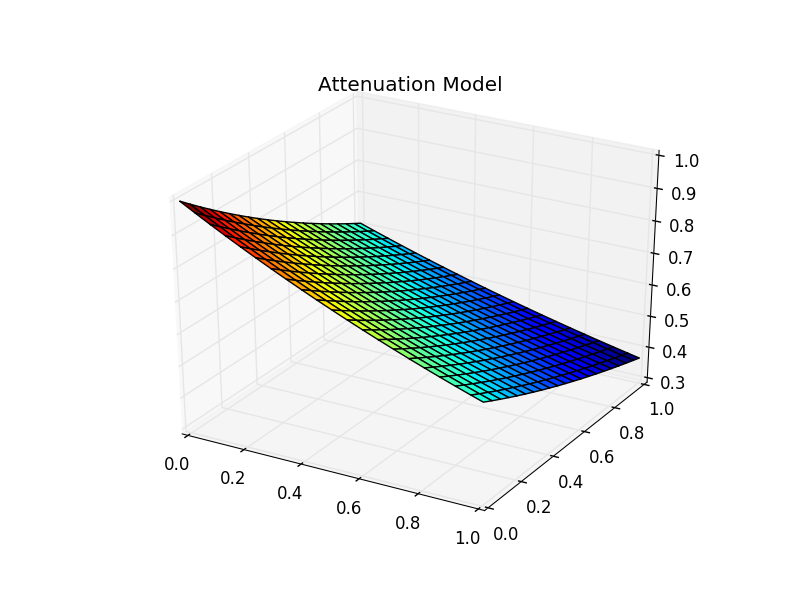
\includegraphics[width=\linewidth]{anlmodels/attenuate}
        \end{figure}
    \end{column}
  \end{columns}
  \begin{itemize}
    \item Tensor of decreasing-importance polynomials
    \item Combination terms over single-variable
  \end{itemize}
\end{frame}
\begin{frame}{SCgPC Results}{Attenuation, Taylor Expansion}%\vspace{-20pt}
  \begin{equation*}
    e^{-ay} = 1 - ay + \frac{(ay)^2}{2} - \frac{(ay)^3}{6} + \frac{(ay)^4}{24} - \frac{(ay)^5}{120} +
          \mathcal{O}(y^6)
  \end{equation*}
\begin{table}
  \centering
  \begin{tabular}{|c c|c c c c c|}
    \cline{3-7}\multicolumn{2}{c|}{ } & \multicolumn{5}{c|}{Polynomial Order ($y_1$)} \\
               \multicolumn{2}{c|}{ } & 0 & 1 & 2 & 3 & 4 \\
    \hline & 0 & 1        & $a$      & $a^2/2$  & $a^3/6$   & \cellcolor{Gray6}$a^4/24$  \\
Polynomial & 1 & $a$      & $a^2   $ & $a^3/2 $ & \cellcolor{Gray6}$a^4/6  $ & $a^5/24 $ \\
Order      & 2 & $a^2/2$  & $a^3/2 $ & \cellcolor{Gray6}$a^4/4 $ & $a^5/12 $ & $a^6/48 $ \\
($y_2$)    & 3 & $a^3/ 6$ & \cellcolor{Gray6}$a^4/ 6$ & $a^5/12$ & $a^6/ 36$ & $a^7/144$ \\
           & 4 & \cellcolor{Gray6}$a^4/24$ & $a^5/24$ & $a^6/48$ & $a^7/144$ & $a^8/576$ \\
    \hline
  \end{tabular}
\end{table}
\end{frame}
\begin{frame}{SCgPC Results}{Attenuation, $N=2$}\vspace{-20pt}
 \begin{columns}
   \begin{column}{0.5\textwidth}
        \begin{figure}[h!]
          \centering
          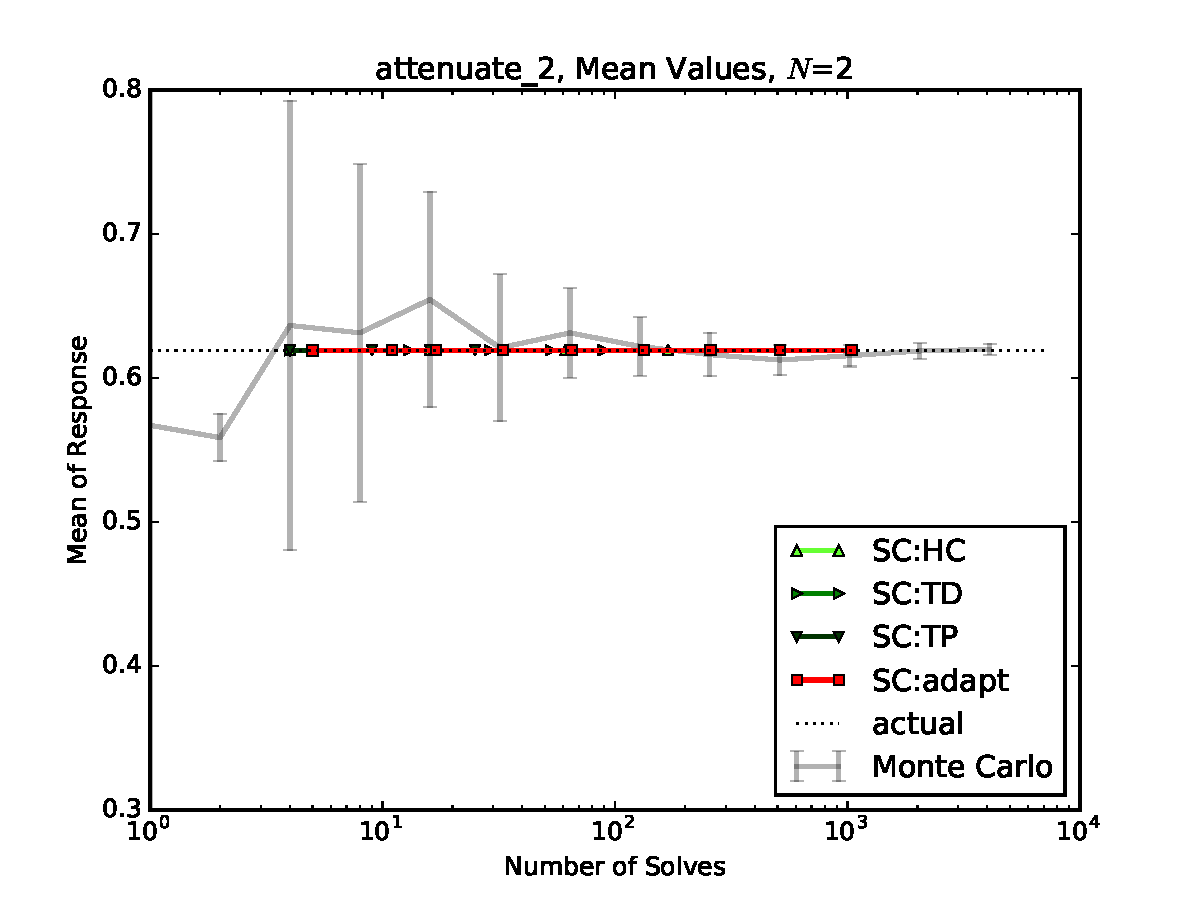
\includegraphics[width=0.8\linewidth]{anlmodels/attenuate_2_mean_vals_nohdmr}
        \end{figure}
        \vspace{-20pt}
        \begin{figure}[h!]
          \centering
          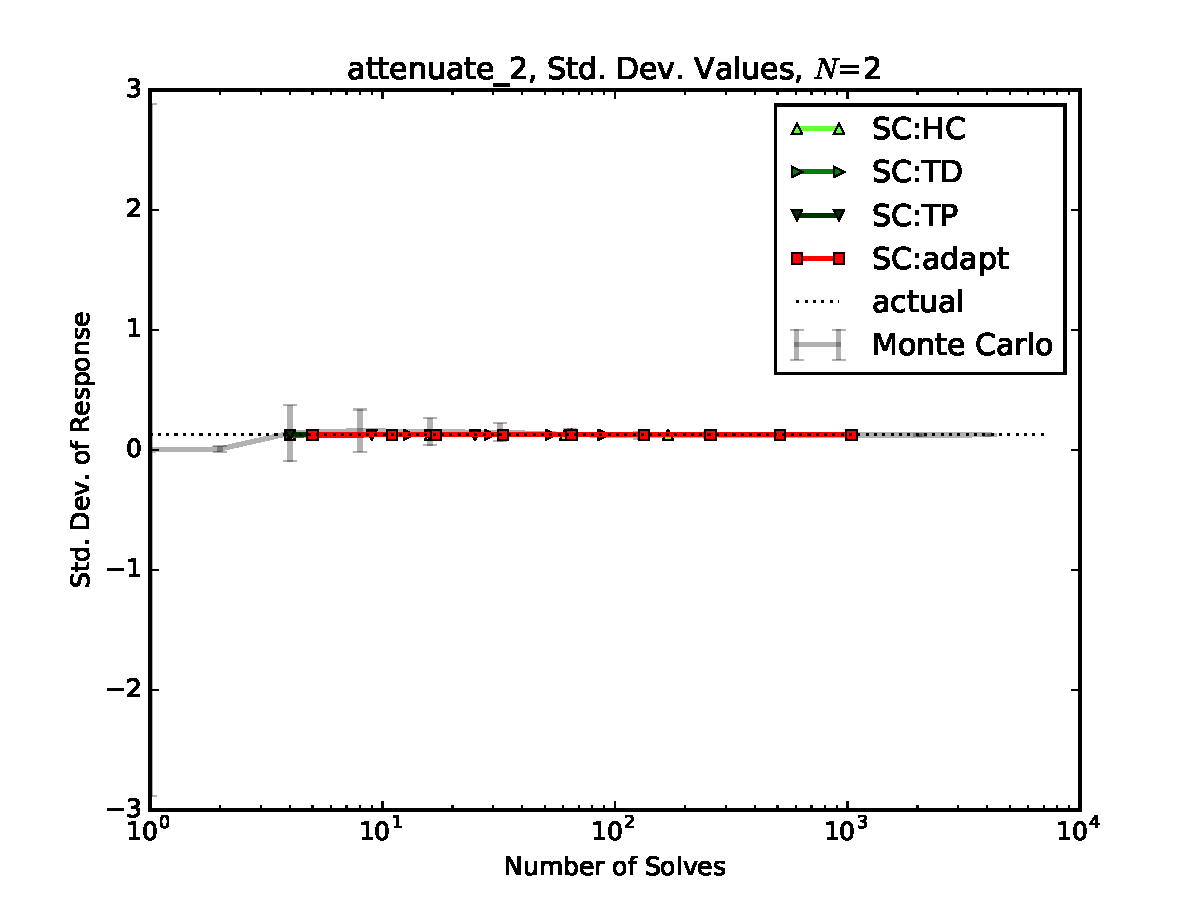
\includegraphics[width=0.8\linewidth]{anlmodels/attenuate_2_var_vals_nohdmr}
        \end{figure}
   \end{column}
   \begin{column}{0.5\textwidth}
        \begin{figure}[h!]
          \centering
          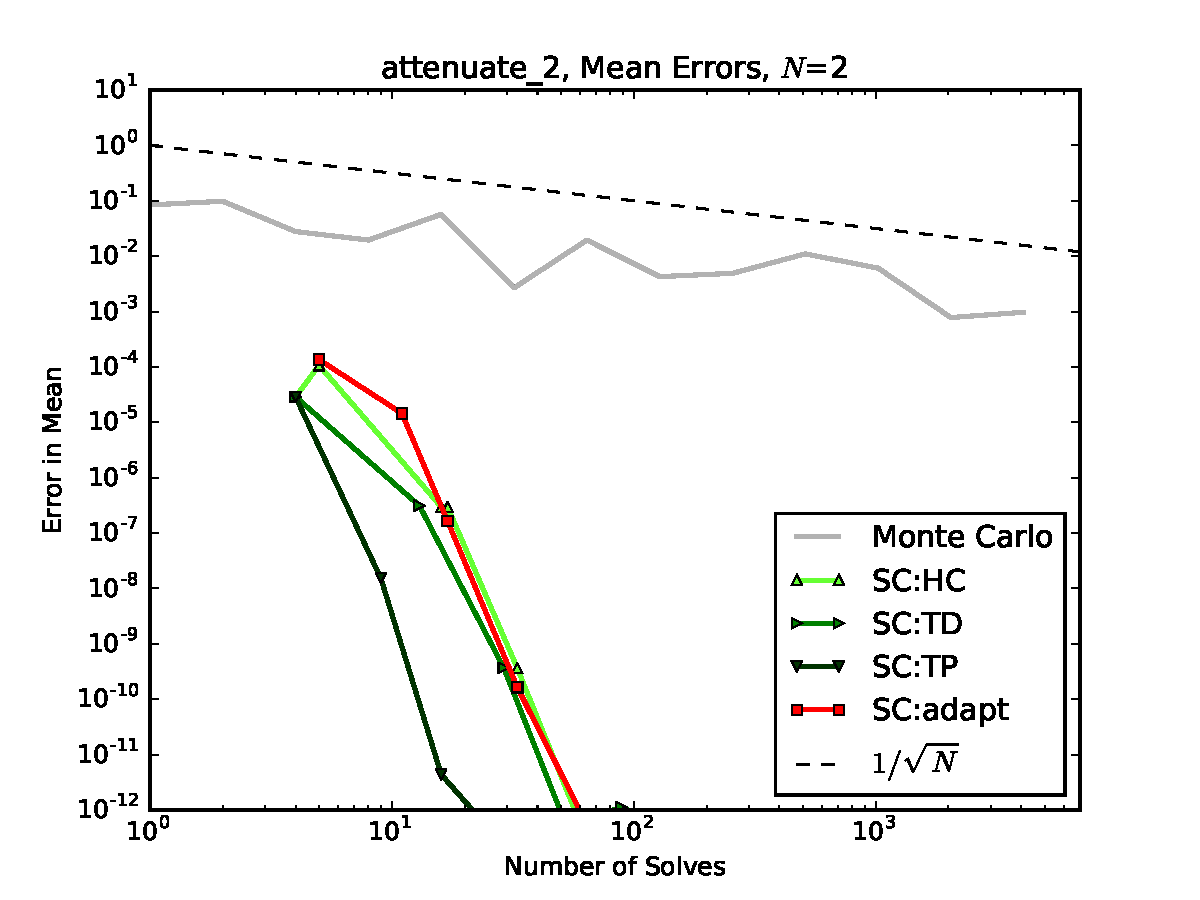
\includegraphics[width=0.8\linewidth]{anlmodels/attenuate_2_mean_errs_nohdmr}
        \end{figure}
        \vspace{-20pt}
        \begin{figure}[h!]
          \centering
          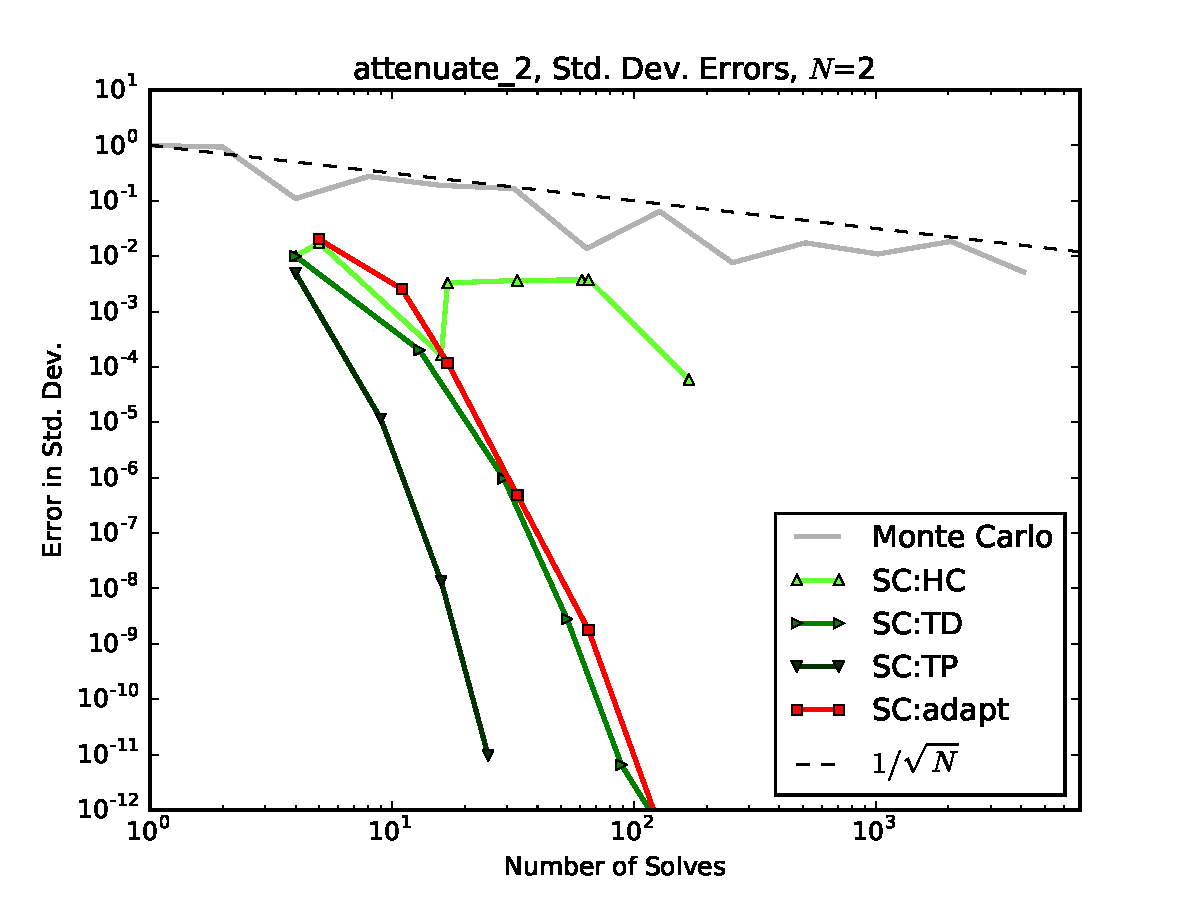
\includegraphics[width=0.8\linewidth]{anlmodels/attenuate_2_variance_errs_nohdmr}
        \end{figure}
   \end{column}
 \end{columns}
\end{frame}
\begin{frame}{SCgPC Results}{Attenuation, $N=4$}\vspace{-20pt}
 \begin{columns}
   \begin{column}{0.5\textwidth}
        \begin{figure}[h!]
          \centering
          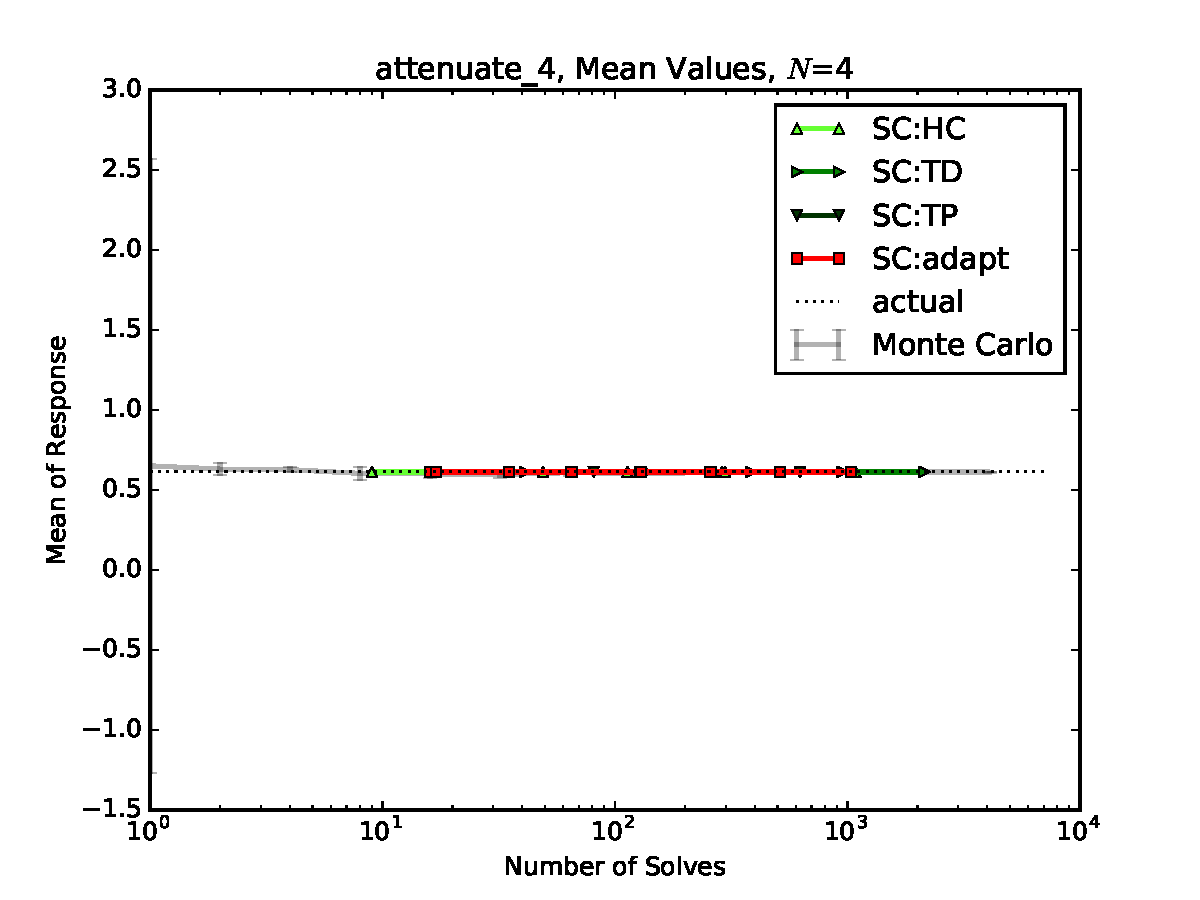
\includegraphics[width=0.8\linewidth]{anlmodels/attenuate_4_mean_vals_nohdmr}
        \end{figure}
        \vspace{-20pt}
        \begin{figure}[h!]
          \centering
          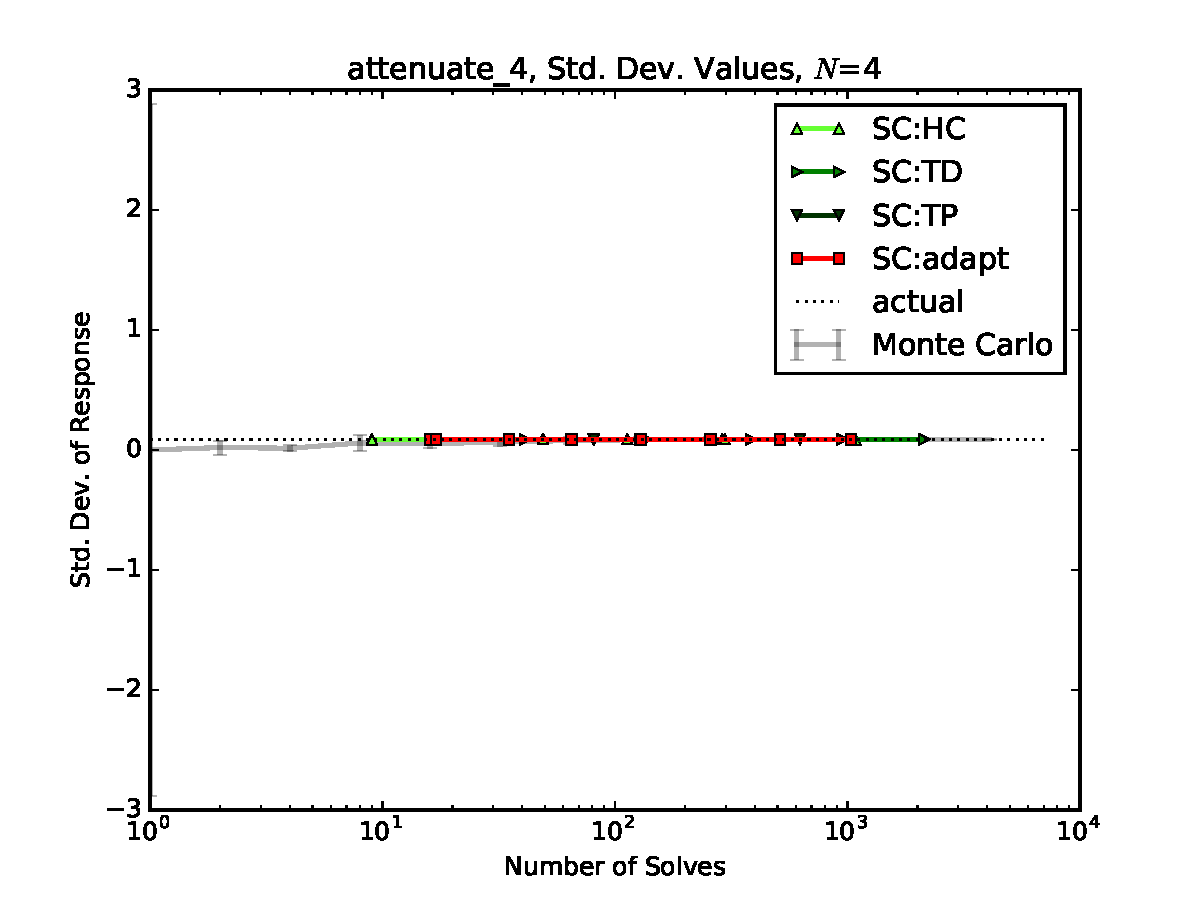
\includegraphics[width=0.8\linewidth]{anlmodels/attenuate_4_var_vals_nohdmr}
        \end{figure}
   \end{column}
   \begin{column}{0.5\textwidth}
        \begin{figure}[h!]
          \centering
          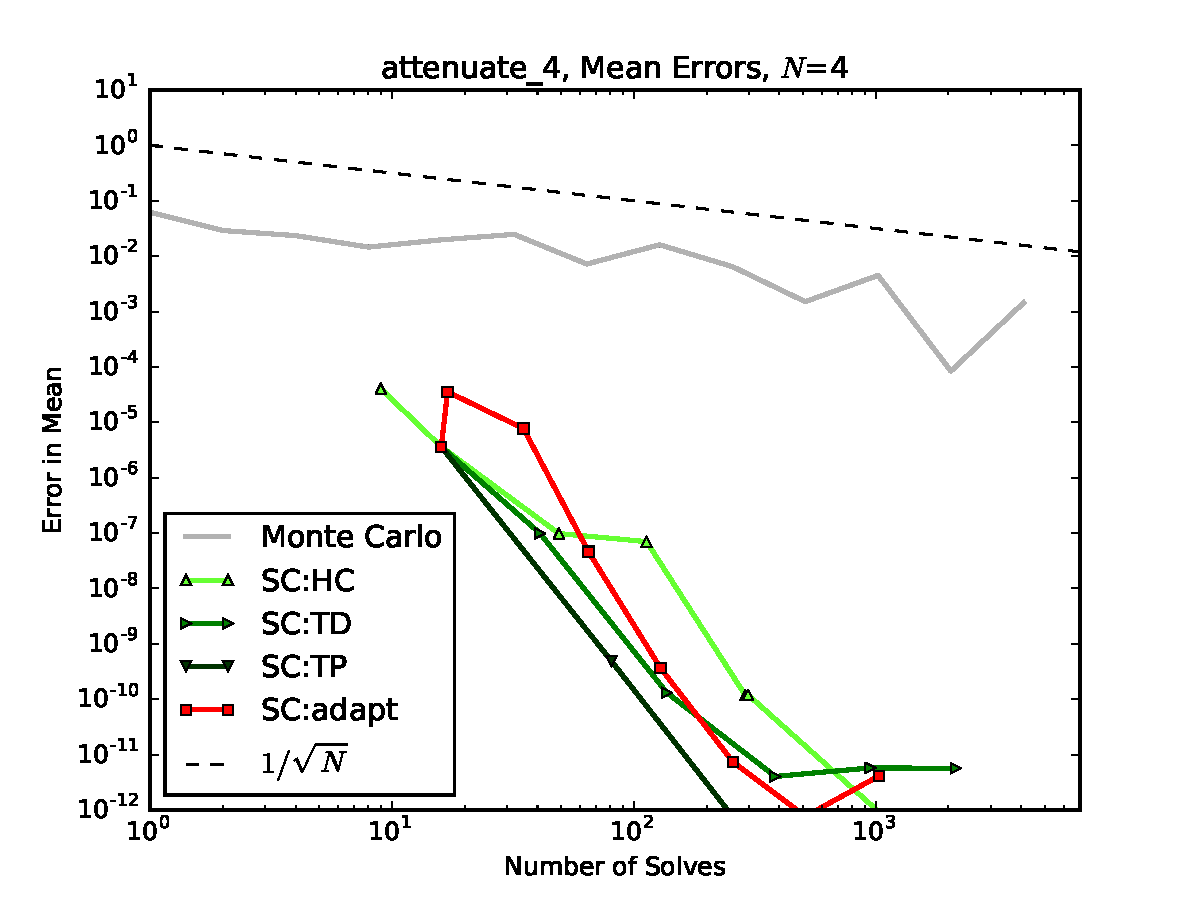
\includegraphics[width=0.8\linewidth]{anlmodels/attenuate_4_mean_errs_nohdmr}
        \end{figure}
        \vspace{-20pt}
        \begin{figure}[h!]
          \centering
          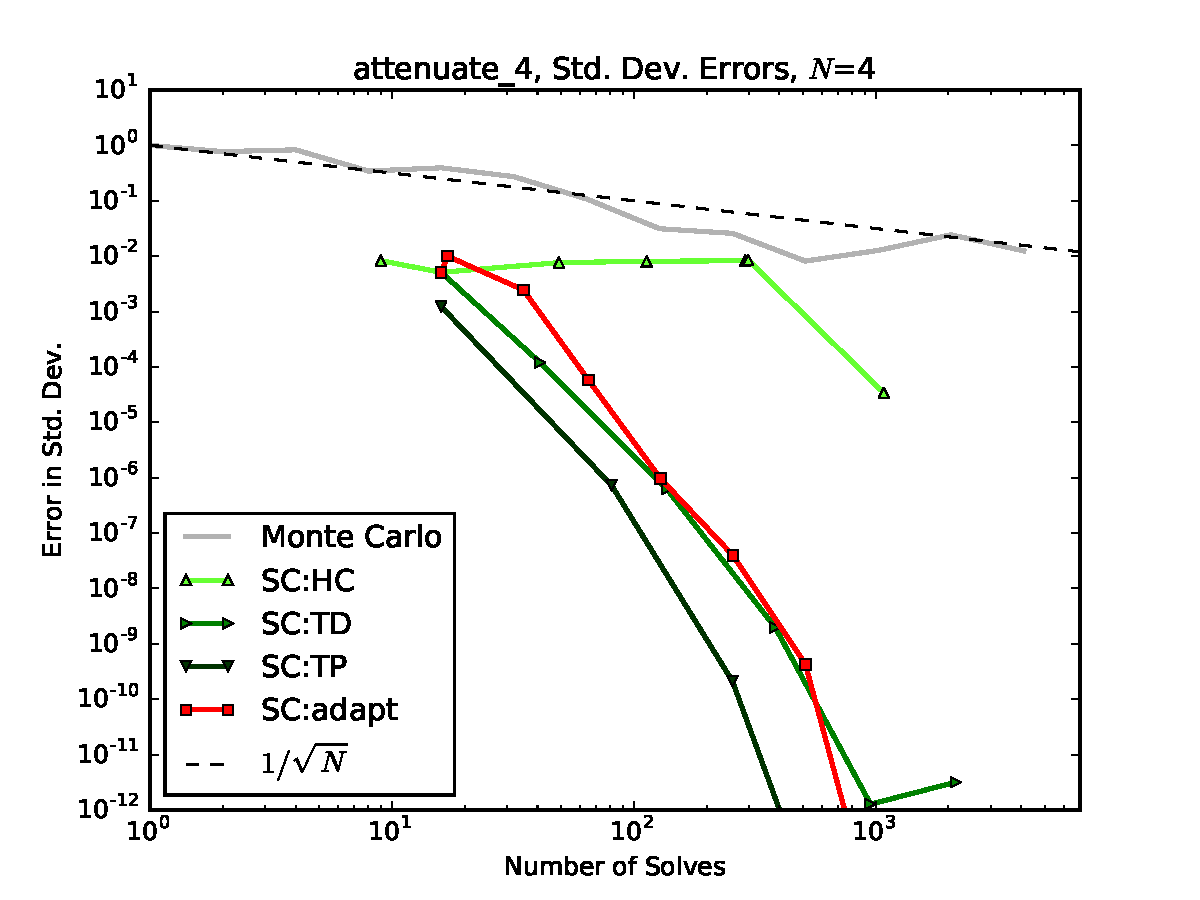
\includegraphics[width=0.8\linewidth]{anlmodels/attenuate_4_variance_errs_nohdmr}
        \end{figure}
   \end{column}
 \end{columns}
\end{frame}
\begin{frame}{SCgPC Results}{Attenuation, $N=6$}\vspace{-20pt}
 \begin{columns}
   \begin{column}{0.5\textwidth}
        \begin{figure}[h!]
          \centering
          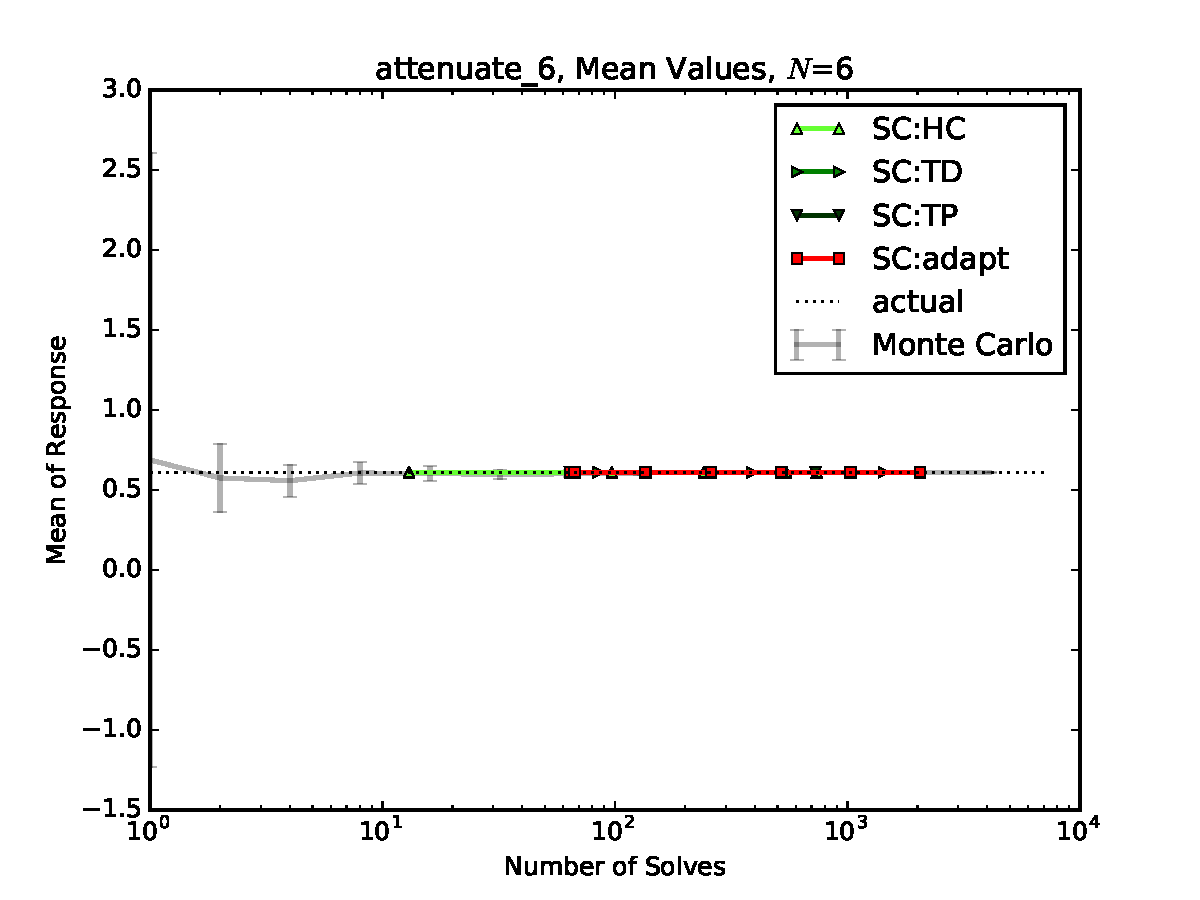
\includegraphics[width=0.8\linewidth]{anlmodels/attenuate_6_mean_vals_nohdmr}
        \end{figure}
        \vspace{-20pt}
        \begin{figure}[h!]
          \centering
          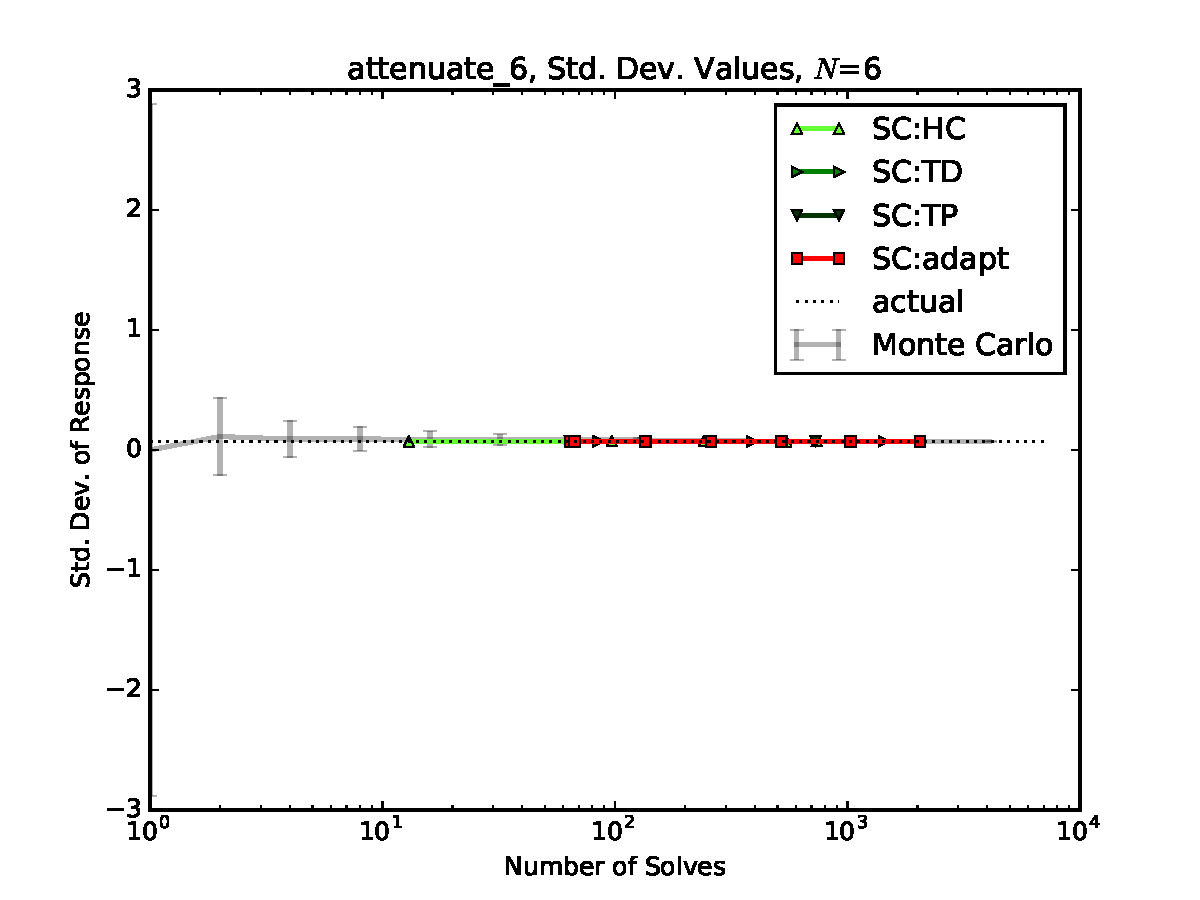
\includegraphics[width=0.8\linewidth]{anlmodels/attenuate_6_var_vals_nohdmr}
        \end{figure}
   \end{column}
   \begin{column}{0.5\textwidth}
        \begin{figure}[h!]
          \centering
          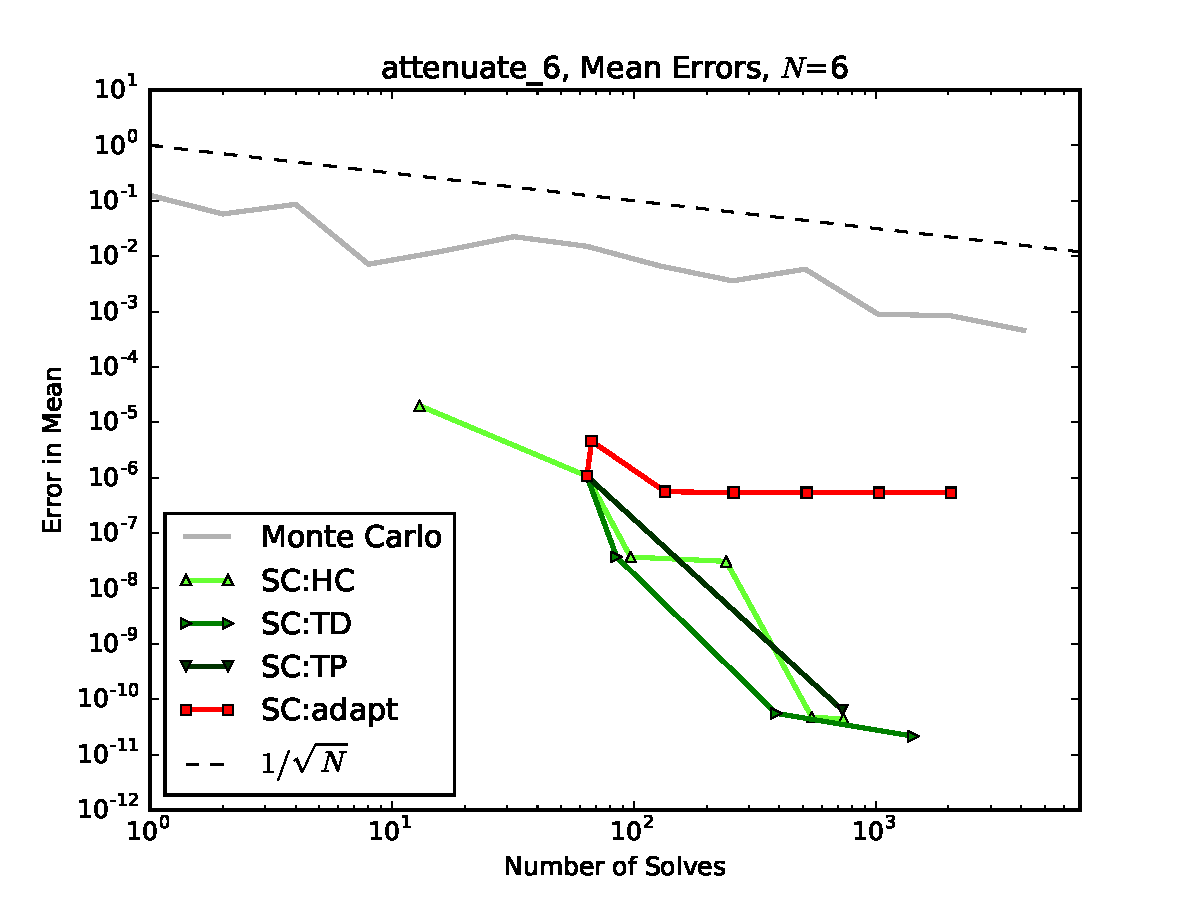
\includegraphics[width=0.8\linewidth]{anlmodels/attenuate_6_mean_errs_nohdmr}
        \end{figure}
        \vspace{-20pt}
        \begin{figure}[h!]
          \centering
          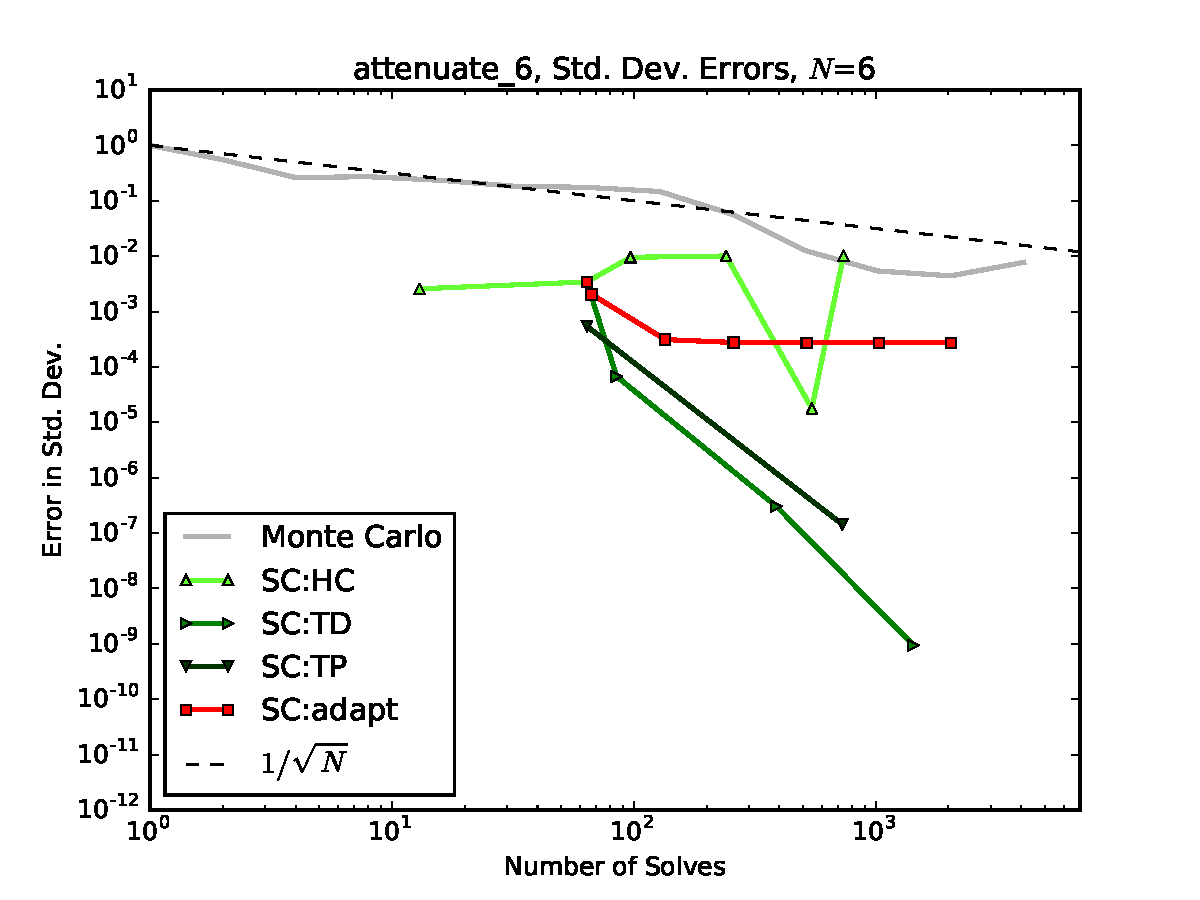
\includegraphics[width=0.8\linewidth]{anlmodels/attenuate_6_variance_errs_nohdmr}
        \end{figure}
   \end{column}
 \end{columns}
\end{frame}




\subsubsection{Gauss Peak}
\begin{frame}{SCgPC Results}{Gauss Peak}\vspace{-20pt}
  \begin{columns}
    \begin{column}{0.6\textwidth}
      \begin{block}{Gauss Peak}
        \[u(Y) = \prod_{n=1}^N \exp(-3^2(y_n-0.5)^2)\]
      \end{block}
    \end{column}
    \begin{column}{0.4\textwidth}
        \begin{figure}[h!]
          \centering
          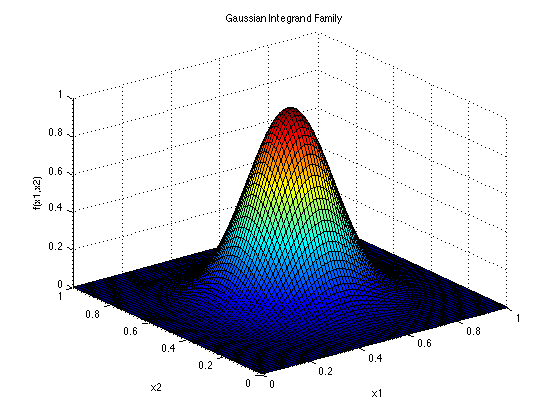
\includegraphics[width=\linewidth]{anlmodels/gaussian}
        \end{figure}
    \end{column}
  \end{columns}
  \begin{itemize}
    \item Tensor of polynomials
    \item Slow, inconsistent decay
  \end{itemize}
\end{frame}
\begin{frame}{SCgPC Results}{Gauss Peak, Taylor Expansion}\vspace{-20pt}
\begin{equation*}
  e^{-a^2y^2} = 1 - a^2y^2 + \frac{a^4}{2}y^4 - \frac{a^6}{6}y^6 + \frac{a^8}{24}y^8 + \mathcal{O}(y^{10})
\end{equation*}
\begin{table}
  \centering
  \begin{tabular}{|c c|c c c c c|}
    \cline{3-7}\multicolumn{2}{c|}{ } & \multicolumn{5}{c|}{Polynomial Order ($y_1$)} \\
\multicolumn{2}{c|}{ } & 0       & 1 & 2       & 3 & 4       \\
    \hline         & 0 & 1       & 0 & $a^2$   & 0 & $a^4/2$ \\
Polynomial         & 1 & 0       & 0 & 0       & 0 & 0       \\
Order              & 2 & $a^2$   & 0 & $a^4$   & 0 & $a^6/2$ \\
($y_2$)            & 3 & 0       & 0 & 0       & 0 & 0       \\
                   & 4 & $a^4/2$ & 0 & $a^6/2$ & 0 & $a^8/4$ \\
    \hline
  \end{tabular}
\end{table}
\end{frame}
\begin{frame}{SCgPC Results}{Gauss Peak, $N=3$}\vspace{-20pt}
 \begin{columns}
   \begin{column}{0.5\textwidth}
        \begin{figure}[h!]
          \centering
          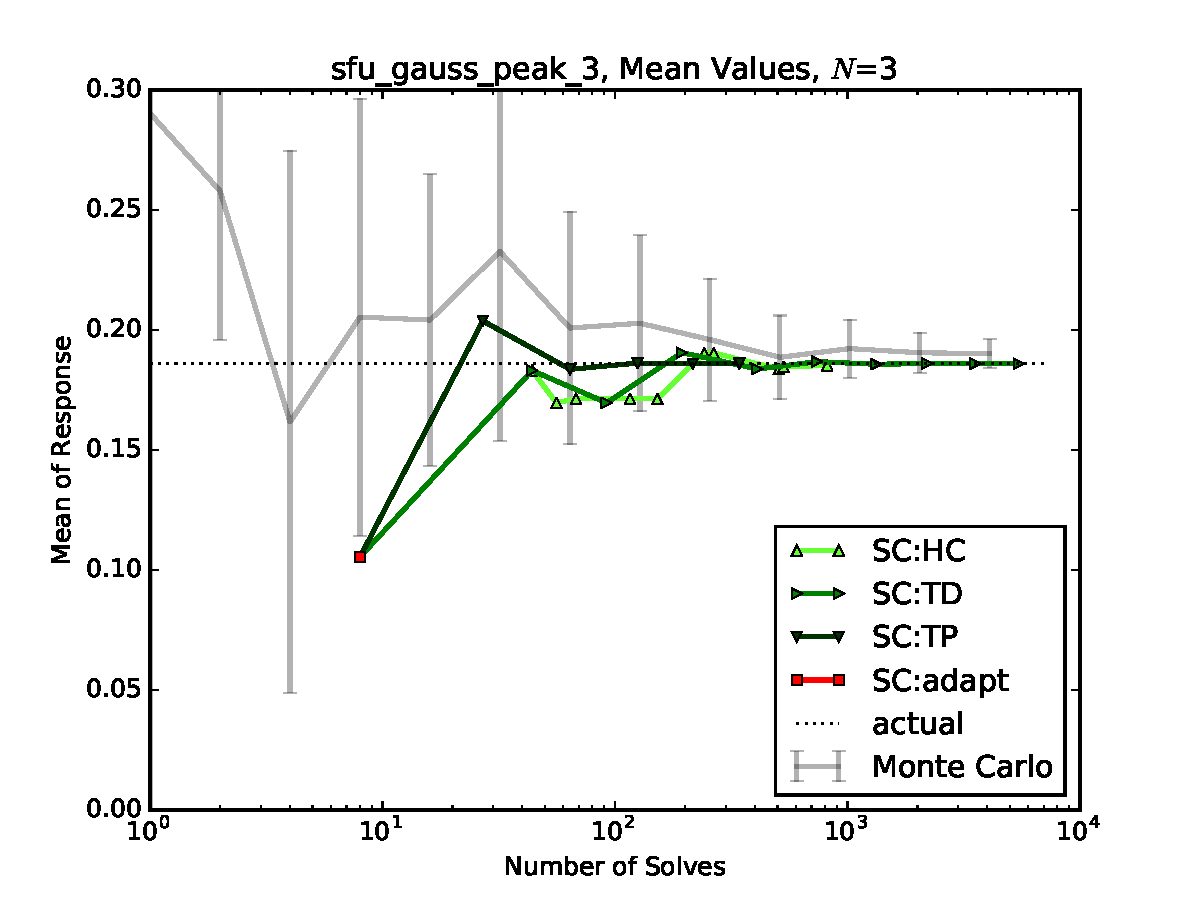
\includegraphics[width=0.8\linewidth]{anlmodels/sfu_gauss_peak_3_mean_vals_nohdmr}
        \end{figure}
        \vspace{-20pt}
        \begin{figure}[h!]
          \centering
          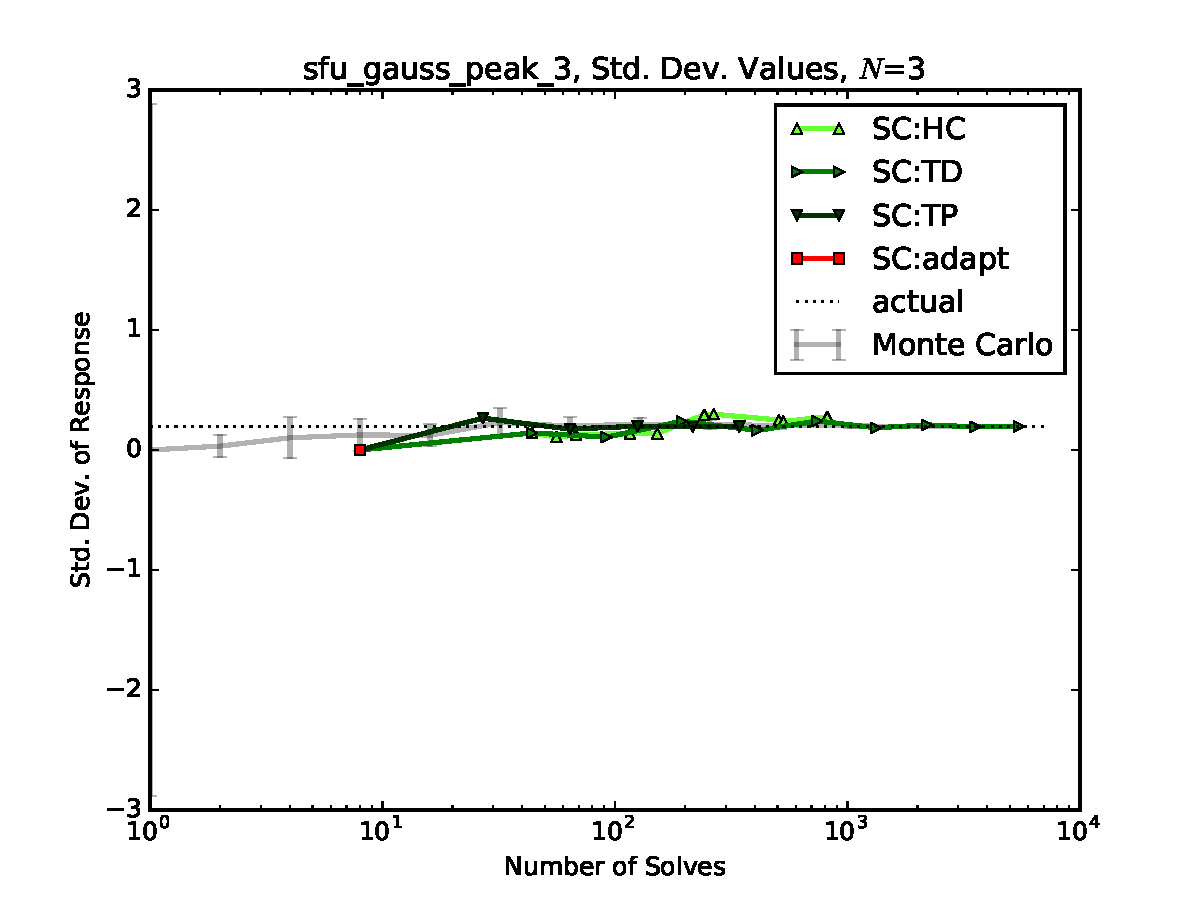
\includegraphics[width=0.8\linewidth]{anlmodels/sfu_gauss_peak_3_var_vals_nohdmr}
        \end{figure}
   \end{column}
   \begin{column}{0.5\textwidth}
        \begin{figure}[h!]
          \centering
          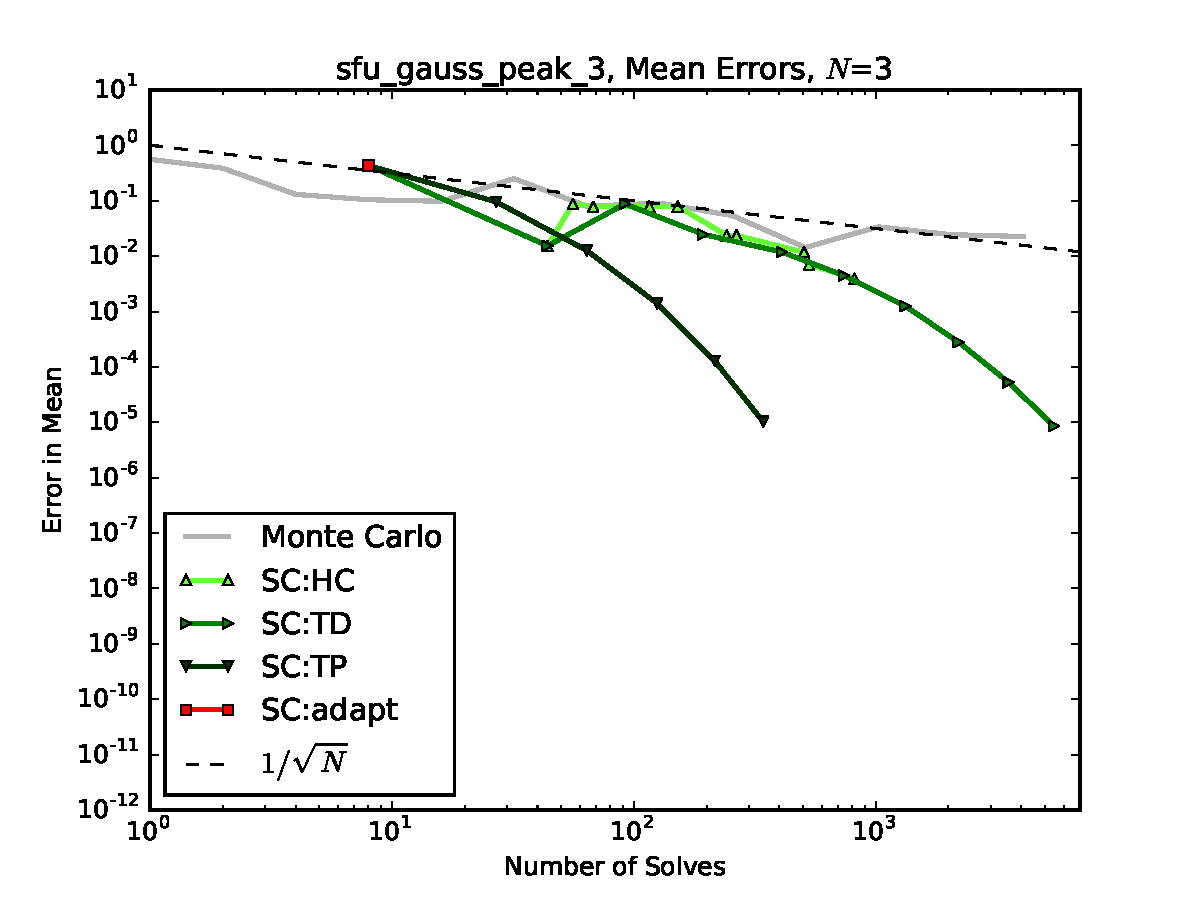
\includegraphics[width=0.8\linewidth]{anlmodels/sfu_gauss_peak_3_mean_errs_nohdmr}
        \end{figure}
        \vspace{-20pt}
        \begin{figure}[h!]
          \centering
          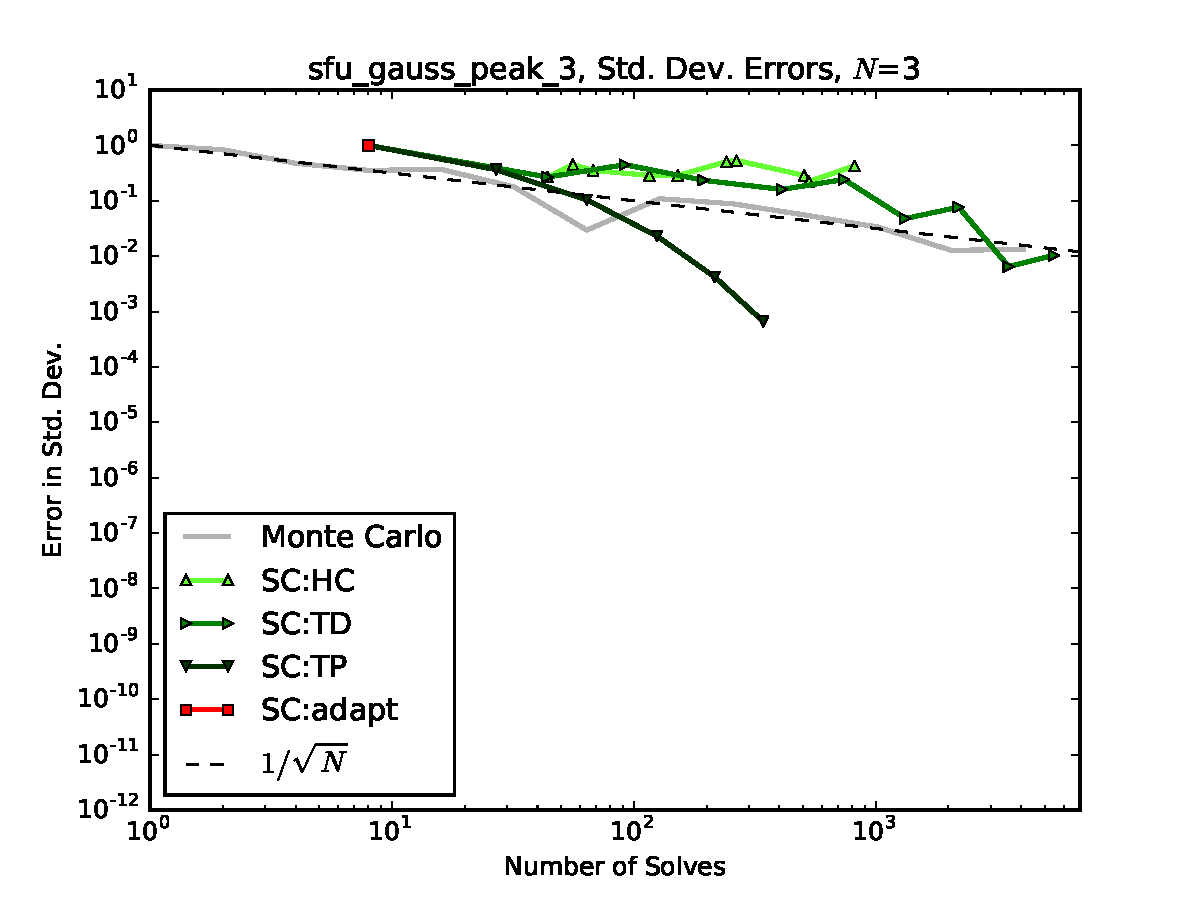
\includegraphics[width=0.8\linewidth]{anlmodels/sfu_gauss_peak_3_variance_errs_nohdmr}
        \end{figure}
   \end{column}
 \end{columns}
\end{frame}
\begin{frame}{SCgPC Results}{Gauss Peak, $N=5$}\vspace{-20pt}
 \begin{columns}
   \begin{column}{0.5\textwidth}
        \begin{figure}[h!]
          \centering
          \includegraphics[width=0.8\linewidth]{anlmodels/sfu_gauss_peak_5_mean_vals_nohdmr}
        \end{figure}
        \vspace{-20pt}
        \begin{figure}[h!]
          \centering
          \includegraphics[width=0.8\linewidth]{anlmodels/sfu_gauss_peak_5_var_vals_nohdmr}
        \end{figure}
   \end{column}
   \begin{column}{0.5\textwidth}
        \begin{figure}[h!]
          \centering
          \includegraphics[width=0.8\linewidth]{anlmodels/sfu_gauss_peak_5_mean_errs_nohdmr}
        \end{figure}
        \vspace{-20pt}
        \begin{figure}[h!]
          \centering
          \includegraphics[width=0.8\linewidth]{anlmodels/sfu_gauss_peak_5_variance_errs_nohdmr}
        \end{figure}
   \end{column}
 \end{columns}
\end{frame}


\subsubsection{Ishigami}
\begin{frame}{SCgPC Results}{Ishigami Function}\vspace{-20pt}
  \begin{columns}
    \begin{column}{0.6\textwidth}
      \begin{block}{Ishigami Function}
        \[u(Y) = \sin{y_1} + a\sin^2{y_2} + b\ y_3^4\sin{y_1}\]
      \end{block}
    \end{column}
    \begin{column}{0.4\textwidth}
        \begin{figure}[h!]
          \centering
          \includegraphics[width=\linewidth]{anlmodels/ishigami}
        \end{figure}
    \end{column}
  \end{columns}
  \begin{itemize}
    \item Not a tensor combination
    \item Strange interplay between $y_1,y_3$
  \end{itemize}
\end{frame}
\begin{frame}{SCgPC Results}{Ishigami Function, Taylor Expansion}\vspace{-20pt}
      \begin{block}{Ishigami Function}
        \[u(Y) = \sin{y_1} + a\sin^2{y_2} + b\ y_3^4\sin{y_1}\]
      \end{block}
\vfill
\begin{equation*}
  \sin{y} = x - \frac{x^3}{6} + \frac{x^5}{120} + \mathcal{O}(x^7)
\end{equation*}
\vfill
\begin{equation*}
  \sin^2{y} = x^2 - \frac{x^4}{3} + \frac{2x^6}{45} + \mathcal{O}(x^8)
\end{equation*}
\vfill
\end{frame}
\begin{frame}{SCgPC Results}{Ishigami Function, $N=3$}\vspace{-20pt}
 \begin{columns}
   \begin{column}{0.5\textwidth}
        \begin{figure}[h!]
          \centering
          \includegraphics[width=0.8\linewidth]{anlmodels/ishigami_3_mean_vals_nohdmr}
        \end{figure}
        \vspace{-20pt}
        \begin{figure}[h!]
          \centering
          \includegraphics[width=0.8\linewidth]{anlmodels/ishigami_3_var_vals_nohdmr}
        \end{figure}
   \end{column}
   \begin{column}{0.5\textwidth}
        \begin{figure}[h!]
          \centering
          \includegraphics[width=0.8\linewidth]{anlmodels/ishigami_3_mean_errs_nohdmr}
        \end{figure}
        \vspace{-20pt}
        \begin{figure}[h!]
          \centering
          \includegraphics[width=0.8\linewidth]{anlmodels/ishigami_3_variance_errs_nohdmr}
        \end{figure}
   \end{column}
 \end{columns}
\end{frame}




\subsubsection{Sobol G-Function}
\begin{frame}{SCgPC Results}{Sobol G-Function}\vspace{-20pt}
  \begin{columns}
    \begin{column}{0.65\textwidth}
      \begin{block}{Sobol G-Function}
        \[u(Y) = \prod_{n=1}^N \frac{|4y_n-2|-a_n}{1+a_n},\hspace{10pt}a_n=\frac{n-2}{2}\]
      \end{block}
    \end{column}
    \begin{column}{0.35\textwidth}
        \begin{figure}[h!]
          \centering
          \includegraphics[width=\linewidth]{anlmodels/gfunc}
        \end{figure}
    \end{column}
  \end{columns}
  \begin{itemize}
    \item Tensor combination of terms
    \item Only zeroth-order continuity
  \end{itemize}
\end{frame}
\begin{frame}{SCgPC Results}{Sobol G-Function, $N=3$}\vspace{-20pt}
 \begin{columns}
   \begin{column}{0.5\textwidth}
        \begin{figure}[h!]
          \centering
          \includegraphics[width=0.8\linewidth]{anlmodels/sobolG_3_mean_vals_nohdmr}
        \end{figure}
        \vspace{-20pt}
        \begin{figure}[h!]
          \centering
          \includegraphics[width=0.8\linewidth]{anlmodels/sobolG_3_var_vals_nohdmr}
        \end{figure}
   \end{column}
   \begin{column}{0.5\textwidth}
        \begin{figure}[h!]
          \centering
          \includegraphics[width=0.8\linewidth]{anlmodels/sobolG_3_mean_errs_nohdmr}
        \end{figure}
        \vspace{-20pt}
        \begin{figure}[h!]
          \centering
          \includegraphics[width=0.8\linewidth]{anlmodels/sobolG_3_variance_errs_nohdmr}
        \end{figure}
   \end{column}
 \end{columns}
\end{frame}
\begin{frame}{SCgPC Results}{Sobol G-Function, $N=5$}\vspace{-20pt}
 \begin{columns}
   \begin{column}{0.5\textwidth}
        \begin{figure}[h!]
          \centering
          \includegraphics[width=0.8\linewidth]{anlmodels/sobolG_5_mean_vals_nohdmr}
        \end{figure}
        \vspace{-20pt}
        \begin{figure}[h!]
          \centering
          \includegraphics[width=0.8\linewidth]{anlmodels/sobolG_5_var_vals_nohdmr}
        \end{figure}
   \end{column}
   \begin{column}{0.5\textwidth}
        \begin{figure}[h!]
          \centering
          \includegraphics[width=0.8\linewidth]{anlmodels/sobolG_5_mean_errs_nohdmr}
        \end{figure}
        \vspace{-20pt}
        \begin{figure}[h!]
          \centering
          \includegraphics[width=0.8\linewidth]{anlmodels/sobolG_5_variance_errs_nohdmr}
        \end{figure}
   \end{column}
 \end{columns}
\end{frame}



%\subsection{SCgPC Conclusions}
\begin{frame}{SCgPC Results}{Conclusions}\vspace{-20pt}
  \vfill
Regarding static SCgPC:
\begin{itemize}
  \item Great in low input space dimensionality
  \item Better with regular responses
  \item Total Degree often great choice
\end{itemize}
  \vfill
Regarding adaptive SCgPC:
\begin{itemize}
  \item Optimal for small input dimensionality
  \item Monotonically-decreasing variance moments
  \item Very poor if oscillating moments
\end{itemize}
  \vfill
\end{frame}

\section{HDMR}
\subsection{Theory}
\begin{frame}{HDMR}{Introduction}%\vspace{-20pt}
  \begin{block}{HDMR Expansion}
    \[u(Y) = H[u](Y) = h_0 + \sum_{n=1}^N h_n + \sum_{n_1=1}^N\sum_{n_2=1}^{n_1-1} h_{n_1,n_2}+\cdots\]
  \end{block}
  \[\hat Y_n \equiv (y_1,\cdots,y_{n-1},y_{n+1},\cdots,y_N)\]
  \[h_0 \equiv \int\limits_\Omega u(Y)\ dY, \hspace{20pt} h_n \equiv \int\limits_{\hat\Omega_n} u(Y)\ d\hat Y_n - h_0\]
\end{frame}

\begin{frame}{HDMR}{HDMR Properties}%\vspace{-20pt}
  \begin{block}{HDMR Expansion}
    \[u(Y) = H[u](Y) = h_0 + \sum_{n=1}^N h_n + \sum_{n_1=1}^N\sum_{n_2=1}^{n_1-1} h_{n_1,n_2}+\cdots\]
  \end{block}
  Properties of HDMR expansion
  \begin{itemize}
    \item Component terms are orthogonal
    \item Contribution of each input to response
    \item Truncates to interaction levels
    \item Sobol sensitivity coefficients
    \item Requires high-level integration even for $h_0$
  \end{itemize}
  \vfill
\end{frame}

\begin{frame}{HDMR}{cut-HDMR}%\vspace{-20pt}
  \begin{block}{Cut-HDMR Expansion}
    \[u(Y) = T[u](Y) = t_r + \sum_{n=1}^N t_n + \sum_{n_1=1}^N\sum_{n_2=1}^{n_1-1} t_{n_1,n_2}+\cdots\]
  \end{block}
  \[\bar Y \equiv (\bar y_1,\cdots,\bar y_N)\]
  \vfill
  \[\hat{\bar{ Y_n}} \equiv (\bar y_1,\cdots,\bar y_{n-1},\bar y_{n+1},\cdots,\bar y_N)\]
  \vfill
  \[t_0 \equiv u(\bar Y), \hspace{20pt} t_n \equiv u(y_n,\hat{\bar{Y_n}}) - t_r\]
  \vfill
\end{frame}

\begin{frame}{HDMR}{Cut-HDMR Properties}%\vspace{-20pt}
  \begin{block}{Cut-HDMR Expansion}
    \[u(Y) = T[u](Y) = t_r + \sum_{n=1}^N t_n + \sum_{n_1=1}^N\sum_{n_2=1}^{n_1-1} t_{n_1,n_2}+\cdots\]
  \end{block}
  \begin{itemize}
    \item No integrals required
    \item Only requires reference value
    \item Terms are no longer orthogonal
    \item Variance is not sum of variance of parts
    \item Converges exactly at no truncation
  \end{itemize}
\end{frame}

\begin{frame}{HDMR}{Cut-HDMR and SCgPC}
  \begin{block}{Cut-HDMR Expansion}
    \[u(Y) = T[u](Y) = t_r + \sum_{n=1}^N t_n + \sum_{n_1=1}^N\sum_{n_2=1}^{n_1-1} t_{n_1,n_2}+\cdots\]
  \end{block}
  Consider subset terms
  \begin{itemize}
    \item Low-dimension input spaces
    \item Potentially regular response
    \item Ideal for SCgPC representation
  \end{itemize}
\end{frame}

\begin{frame}{HDMR}{Cut-HDMR and SCgPC}
  \begin{block}{Cut-HDMR Expansion}
    \[u(Y) = T[u](Y) = t_r + \sum_{n=1}^N t_n + \sum_{n_1=1}^N\sum_{n_2=1}^{n_1-1} t_{n_1,n_2}+\cdots\]
  \end{block}\vspace{-20pt}
  \begin{align*}
    t_n &= G[u](y_n,\hat{\bar{Y_n}}) - t_r \\
    &= \sum_{k'\in\Lambda'(L')} t_{n;k'}\Phi_{k'}(y_n) - t_r
  \end{align*}
  \begin{itemize}
    \item $t_{n;k'}$ calculated with Smolyak collocation
    \item Orthonormality re-introduced
    \item Can algorithmically recover ANOVA HDMR
  \end{itemize}
\end{frame}

\begin{frame}{HDMR}{Cut-HDMR and SCgPC versus SCgPC}
  \vfill
  Is cut-HDMR with SCgPC better than SCgPC alone?
  \vfill
  \begin{itemize}
    \item Using same polynomial orders and families
  \vfill
    \item Using same index set type $\Lambda$
  \vfill
    \item Untruncated cut-HDMR is same as SCgPC
  \vfill
    \item Truncated can approximate with less evaluations
  \vfill
    \item Most effective when solves very expensive
  \end{itemize}
  \vfill
\end{frame}

\subsection{Results}
\begin{frame}{HDMR Results}{Introduction}\vspace{-20pt}
  \vfill
  Contrast HDMR with SCgPC
  \vfill
  \begin{itemize}
    \item Same analytic models
  \vfill
    \item First-, second-, third-order HDMR
  \vfill
    \item Adaptive HDMR with adaptive SCgPC
  \end{itemize}
  \vfill
\end{frame}

\subsubsection{Tensor Monomials}
\begin{frame}{HDMR Results}{Tensor Monomials}\vspace{-20pt}
  \begin{columns}
    \begin{column}{0.6\textwidth}
      \begin{block}{Tensor Monomials}
        \[u(Y) = \prod_{n=1}^N (y_n+1)\]
      \end{block}
    \end{column}
    \begin{column}{0.4\textwidth}
        \begin{figure}[h!]
          \centering
          \includegraphics[width=\linewidth]{anlmodels/tensor_monom}
        \end{figure}
    \end{column}
  \end{columns}
  \begin{itemize}
    \item Linear response
    \item All polynomial combinations
  \end{itemize}
\end{frame}
\begin{frame}{HDMR Results}{Tensor Monomials, $N=3$}\vspace{-20pt}
 \begin{columns}
   \begin{column}{0.5\textwidth}
        \begin{figure}[h!]
          \centering
          \includegraphics[width=0.8\linewidth]{anlmodels/tensor_monomial_3_mean_vals}
        \end{figure}
        \vspace{-20pt}
        \begin{figure}[h!]
          \centering
          \includegraphics[width=0.8\linewidth]{anlmodels/tensor_monomial_3_var_vals}
        \end{figure}
   \end{column}
   \begin{column}{0.5\textwidth}
        \begin{figure}[h!]
          \centering
          \includegraphics[width=0.8\linewidth]{anlmodels/tensor_monomial_3_mean_errs}
        \end{figure}
        \vspace{-20pt}
        \begin{figure}[h!]
          \centering
          \includegraphics[width=0.8\linewidth]{anlmodels/tensor_monomial_3_variance_errs}
        \end{figure}
   \end{column}
 \end{columns}
\end{frame}
\begin{frame}{HDMR Results}{Tensor Monomials, $N=5$}\vspace{-20pt}
 \begin{columns}
   \begin{column}{0.5\textwidth}
        \begin{figure}[h!]
          \centering
          \includegraphics[width=0.8\linewidth]{anlmodels/tensor_monomial_5_mean_vals}
        \end{figure}
        \vspace{-20pt}
        \begin{figure}[h!]
          \centering
          \includegraphics[width=0.8\linewidth]{anlmodels/tensor_monomial_5_var_vals}
        \end{figure}
   \end{column}
   \begin{column}{0.5\textwidth}
        \begin{figure}[h!]
          \centering
          \includegraphics[width=0.8\linewidth]{anlmodels/tensor_monomial_5_mean_errs}
        \end{figure}
        \vspace{-20pt}
        \begin{figure}[h!]
          \centering
          \includegraphics[width=0.8\linewidth]{anlmodels/tensor_monomial_5_variance_errs}
        \end{figure}
   \end{column}
 \end{columns}
\end{frame}
\begin{frame}{HDMR Results}{Tensor Monomials, $N=10$}\vspace{-20pt}
 \begin{columns}
   \begin{column}{0.5\textwidth}
        \begin{figure}[h!]
          \centering
          \includegraphics[width=0.8\linewidth]{anlmodels/tensor_monomial_10_mean_vals}
        \end{figure}
        \vspace{-20pt}
        \begin{figure}[h!]
          \centering
          \includegraphics[width=0.8\linewidth]{anlmodels/tensor_monomial_10_var_vals}
        \end{figure}
   \end{column}
   \begin{column}{0.5\textwidth}
        \begin{figure}[h!]
          \centering
          \includegraphics[width=0.8\linewidth]{anlmodels/tensor_monomial_10_mean_errs}
        \end{figure}
        \vspace{-20pt}
        \begin{figure}[h!]
          \centering
          \includegraphics[width=0.8\linewidth]{anlmodels/tensor_monomial_10_variance_errs}
        \end{figure}
   \end{column}
 \end{columns}
\end{frame}



\subsubsection{Sudret Polynomial}
\begin{frame}{HDMR Results}{Sudret Polynomials}\vspace{-20pt}
  \begin{columns}
    \begin{column}{0.6\textwidth}
      \begin{block}{Sudret Polynomials}
        \[u(Y) = \frac{1}{2^N}\prod_{n=1}^N (3y_n^2+1)\]
      \end{block}
    \end{column}
    \begin{column}{0.4\textwidth}
        \begin{figure}[h!]
          \centering
          \includegraphics[width=\linewidth]{anlmodels/sudret}
        \end{figure}
    \end{column}
  \end{columns}
  \begin{itemize}
    \item Exclusively second-order interactions
    \item All second-order polynomial combinations
  \end{itemize}
\end{frame}
\begin{frame}{HDMR Results}{Sudret Polynomials, $N=3$}\vspace{-20pt}
 \begin{columns}
   \begin{column}{0.5\textwidth}
        \begin{figure}[h!]
          \centering
          \includegraphics[width=0.8\linewidth]{anlmodels/sudret_3_mean_vals}
        \end{figure}
        \vspace{-20pt}
        \begin{figure}[h!]
          \centering
          \includegraphics[width=0.8\linewidth]{anlmodels/sudret_3_var_vals}
        \end{figure}
   \end{column}
   \begin{column}{0.5\textwidth}
        \begin{figure}[h!]
          \centering
          \includegraphics[width=0.8\linewidth]{anlmodels/sudret_3_mean_errs}
        \end{figure}
        \vspace{-20pt}
        \begin{figure}[h!]
          \centering
          \includegraphics[width=0.8\linewidth]{anlmodels/sudret_3_variance_errs}
        \end{figure}
   \end{column}
 \end{columns}
\end{frame}
\begin{frame}{HDMR Results}{Sudret Polynomials, $N=5$}\vspace{-20pt}
 \begin{columns}
   \begin{column}{0.5\textwidth}
        \begin{figure}[h!]
          \centering
          \includegraphics[width=0.8\linewidth]{anlmodels/sudret_5_mean_vals}
        \end{figure}
        \vspace{-20pt}
        \begin{figure}[h!]
          \centering
          \includegraphics[width=0.8\linewidth]{anlmodels/sudret_5_var_vals}
        \end{figure}
   \end{column}
   \begin{column}{0.5\textwidth}
        \begin{figure}[h!]
          \centering
          \includegraphics[width=0.8\linewidth]{anlmodels/sudret_5_mean_errs}
        \end{figure}
        \vspace{-20pt}
        \begin{figure}[h!]
          \centering
          \includegraphics[width=0.8\linewidth]{anlmodels/sudret_5_variance_errs}
        \end{figure}
   \end{column}
 \end{columns}
\end{frame}


\subsubsection{Attenuation}
\begin{frame}{HDMR Results}{Attenuation}\vspace{-20pt}
  \begin{columns}
    \begin{column}{0.6\textwidth}
      \begin{block}{Attenuation}
        \[u(Y) = \prod_{n=1}^N \exp(-y_n/N)\]
      \end{block}
    \end{column}
    \begin{column}{0.4\textwidth}
        \begin{figure}[h!]
          \centering
          \includegraphics[width=\linewidth]{anlmodels/attenuate}
        \end{figure}
    \end{column}
  \end{columns}
  \begin{itemize}
    \item Tensor of decreasing-importance polynomials
    \item Combination terms over single-variable
  \end{itemize}
\end{frame}
\begin{frame}{HDMR Results}{Attenuation, Taylor Expansion}%\vspace{-20pt}
  \begin{equation*}
    e^{-ay} = 1 - ay + \frac{(ay)^2}{2} - \frac{(ay)^3}{6} + \frac{(ay)^4}{24} - \frac{(ay)^5}{120} +
          \mathcal{O}(y^6)
  \end{equation*}
\begin{table}
  \centering
  \begin{tabular}{|c c|c c c c c|}
    \cline{3-7}\multicolumn{2}{c|}{ } & \multicolumn{5}{c|}{Polynomial Order ($y_1$)} \\
               \multicolumn{2}{c|}{ } & 0 & 1 & 2 & 3 & 4 \\
    \hline & 0 & 1        & $a$      & $a^2/2$  & $a^3/6$   & \cellcolor{Gray6}$a^4/24$  \\
Polynomial & 1 & $a$      & $a^2   $ & $a^3/2 $ & \cellcolor{Gray6}$a^4/6  $ & $a^5/24 $ \\
Order      & 2 & $a^2/2$  & $a^3/2 $ & \cellcolor{Gray6}$a^4/4 $ & $a^5/12 $ & $a^6/48 $ \\
($y_2$)    & 3 & $a^3/ 6$ & \cellcolor{Gray6}$a^4/ 6$ & $a^5/12$ & $a^6/ 36$ & $a^7/144$ \\
           & 4 & \cellcolor{Gray6}$a^4/24$ & $a^5/24$ & $a^6/48$ & $a^7/144$ & $a^8/576$ \\
    \hline
  \end{tabular}
\end{table}
\end{frame}
\begin{frame}{HDMR Results}{Attenuation, $N=2$}\vspace{-20pt}
 \begin{columns}
   \begin{column}{0.5\textwidth}
        \begin{figure}[h!]
          \centering
          \includegraphics[width=0.8\linewidth]{anlmodels/attenuate_2_mean_vals}
        \end{figure}
        \vspace{-20pt}
        \begin{figure}[h!]
          \centering
          \includegraphics[width=0.8\linewidth]{anlmodels/attenuate_2_var_vals}
        \end{figure}
   \end{column}
   \begin{column}{0.5\textwidth}
        \begin{figure}[h!]
          \centering
          \includegraphics[width=0.8\linewidth]{anlmodels/attenuate_2_mean_errs}
        \end{figure}
        \vspace{-20pt}
        \begin{figure}[h!]
          \centering
          \includegraphics[width=0.8\linewidth]{anlmodels/attenuate_2_variance_errs}
        \end{figure}
   \end{column}
 \end{columns}
\end{frame}
\begin{frame}{HDMR Results}{Attenuation, $N=4$}\vspace{-20pt}
 \begin{columns}
   \begin{column}{0.5\textwidth}
        \begin{figure}[h!]
          \centering
          \includegraphics[width=0.8\linewidth]{anlmodels/attenuate_4_mean_vals}
        \end{figure}
        \vspace{-20pt}
        \begin{figure}[h!]
          \centering
          \includegraphics[width=0.8\linewidth]{anlmodels/attenuate_4_var_vals}
        \end{figure}
   \end{column}
   \begin{column}{0.5\textwidth}
        \begin{figure}[h!]
          \centering
          \includegraphics[width=0.8\linewidth]{anlmodels/attenuate_4_mean_errs}
        \end{figure}
        \vspace{-20pt}
        \begin{figure}[h!]
          \centering
          \includegraphics[width=0.8\linewidth]{anlmodels/attenuate_4_variance_errs}
        \end{figure}
   \end{column}
 \end{columns}
\end{frame}
\begin{frame}{HDMR Results}{Attenuation, $N=6$}\vspace{-20pt}
 \begin{columns}
   \begin{column}{0.5\textwidth}
        \begin{figure}[h!]
          \centering
          \includegraphics[width=0.8\linewidth]{anlmodels/attenuate_6_mean_vals}
        \end{figure}
        \vspace{-20pt}
        \begin{figure}[h!]
          \centering
          \includegraphics[width=0.8\linewidth]{anlmodels/attenuate_6_var_vals}
        \end{figure}
   \end{column}
   \begin{column}{0.5\textwidth}
        \begin{figure}[h!]
          \centering
          \includegraphics[width=0.8\linewidth]{anlmodels/attenuate_6_mean_errs}
        \end{figure}
        \vspace{-20pt}
        \begin{figure}[h!]
          \centering
          \includegraphics[width=0.8\linewidth]{anlmodels/attenuate_6_variance_errs}
        \end{figure}
   \end{column}
 \end{columns}
\end{frame}




\subsubsection{Gauss Peak}
\begin{frame}{HDMR Results}{Gauss Peak}\vspace{-20pt}
  \begin{columns}
    \begin{column}{0.6\textwidth}
      \begin{block}{Gauss Peak}
        \[u(Y) = \prod_{n=1}^N \exp(-3^2(y_n-0.5)^2)\]
      \end{block}
    \end{column}
    \begin{column}{0.4\textwidth}
        \begin{figure}[h!]
          \centering
          \includegraphics[width=\linewidth]{anlmodels/gaussian}
        \end{figure}
    \end{column}
  \end{columns}
  \begin{itemize}
    \item Tensor of polynomials
    \item Slow, inconsistent decay
  \end{itemize}
\end{frame}
\begin{frame}{HDMR Results}{Gauss Peak, Taylor Expansion}\vspace{-20pt}
\begin{equation*}
  e^{-a^2y^2} = 1 - a^2y^2 + \frac{a^4}{2}y^4 - \frac{a^6}{6}y^6 + \frac{a^8}{24}y^8 + \mathcal{O}(y^{10})
\end{equation*}
\begin{table}
  \centering
  \begin{tabular}{|c c|c c c c c|}
    \cline{3-7}\multicolumn{2}{c|}{ } & \multicolumn{5}{c|}{Polynomial Order ($y_1$)} \\
\multicolumn{2}{c|}{ } & 0       & 1 & 2       & 3 & 4       \\
    \hline         & 0 & 1       & 0 & $a^2$   & 0 & $a^4/2$ \\
Polynomial         & 1 & 0       & 0 & 0       & 0 & 0       \\
Order              & 2 & $a^2$   & 0 & $a^4$   & 0 & $a^6/2$ \\
($y_2$)            & 3 & 0       & 0 & 0       & 0 & 0       \\
                   & 4 & $a^4/2$ & 0 & $a^6/2$ & 0 & $a^8/4$ \\
    \hline
  \end{tabular}
\end{table}
\end{frame}
\begin{frame}{HDMR Results}{Gauss Peak, $N=3$}\vspace{-20pt}
 \begin{columns}
   \begin{column}{0.5\textwidth}
        \begin{figure}[h!]
          \centering
          \includegraphics[width=0.8\linewidth]{anlmodels/sfu_gauss_peak_3_mean_vals}
        \end{figure}
        \vspace{-20pt}
        \begin{figure}[h!]
          \centering
          \includegraphics[width=0.8\linewidth]{anlmodels/sfu_gauss_peak_3_var_vals}
        \end{figure}
   \end{column}
   \begin{column}{0.5\textwidth}
        \begin{figure}[h!]
          \centering
          \includegraphics[width=0.8\linewidth]{anlmodels/sfu_gauss_peak_3_mean_errs}
        \end{figure}
        \vspace{-20pt}
        \begin{figure}[h!]
          \centering
          \includegraphics[width=0.8\linewidth]{anlmodels/sfu_gauss_peak_3_variance_errs}
        \end{figure}
   \end{column}
 \end{columns}
\end{frame}
\begin{frame}{HDMR Results}{Gauss Peak, $N=5$}\vspace{-20pt}
 \begin{columns}
   \begin{column}{0.5\textwidth}
        \begin{figure}[h!]
          \centering
          \includegraphics[width=0.8\linewidth]{anlmodels/sfu_gauss_peak_5_mean_vals}
        \end{figure}
        \vspace{-20pt}
        \begin{figure}[h!]
          \centering
          \includegraphics[width=0.8\linewidth]{anlmodels/sfu_gauss_peak_5_var_vals}
        \end{figure}
   \end{column}
   \begin{column}{0.5\textwidth}
        \begin{figure}[h!]
          \centering
          \includegraphics[width=0.8\linewidth]{anlmodels/sfu_gauss_peak_5_mean_errs}
        \end{figure}
        \vspace{-20pt}
        \begin{figure}[h!]
          \centering
          \includegraphics[width=0.8\linewidth]{anlmodels/sfu_gauss_peak_5_variance_errs}
        \end{figure}
   \end{column}
 \end{columns}
\end{frame}


\subsubsection{Ishigami}
\begin{frame}{HDMR Results}{Ishigami Function}\vspace{-20pt}
  \begin{columns}
    \begin{column}{0.6\textwidth}
      \begin{block}{Ishigami Function}
        \[u(Y) = \sin{y_1} + a\sin^2{y_2} + b\ y_3^4\sin{y_1}\]
      \end{block}
    \end{column}
    \begin{column}{0.4\textwidth}
        \begin{figure}[h!]
          \centering
          \includegraphics[width=\linewidth]{anlmodels/ishigami}
        \end{figure}
    \end{column}
  \end{columns}
  \begin{itemize}
    \item Not a tensor combination
    \item Strange interplay between $y_1,y_3$
  \end{itemize}
\end{frame}
\begin{frame}{HDMR Results}{Ishigami Function, Taylor Expansion}\vspace{-20pt}
      \begin{block}{Ishigami Function}
        \[u(Y) = \sin{y_1} + a\sin^2{y_2} + b\ y_3^4\sin{y_1}\]
      \end{block}
\vfill
\begin{equation*}
  \sin{y} = x - \frac{x^3}{6} + \frac{x^5}{120} + \mathcal{O}(x^7)
\end{equation*}
\vfill
\begin{equation*}
  \sin^2{y} = x^2 - \frac{x^4}{3} + \frac{2x^6}{45} + \mathcal{O}(x^8)
\end{equation*}
\vfill
\end{frame}
\begin{frame}{HDMR Results}{Ishigami Function, $N=3$}\vspace{-20pt}
 \begin{columns}
   \begin{column}{0.5\textwidth}
        \begin{figure}[h!]
          \centering
          \includegraphics[width=0.8\linewidth]{anlmodels/ishigami_3_mean_vals}
        \end{figure}
        \vspace{-20pt}
        \begin{figure}[h!]
          \centering
          \includegraphics[width=0.8\linewidth]{anlmodels/ishigami_3_var_vals}
        \end{figure}
   \end{column}
   \begin{column}{0.5\textwidth}
        \begin{figure}[h!]
          \centering
          \includegraphics[width=0.8\linewidth]{anlmodels/ishigami_3_mean_errs}
        \end{figure}
        \vspace{-20pt}
        \begin{figure}[h!]
          \centering
          \includegraphics[width=0.8\linewidth]{anlmodels/ishigami_3_variance_errs}
        \end{figure}
   \end{column}
 \end{columns}
\end{frame}




\subsubsection{Sobol G-Function}
\begin{frame}{HDMR Results}{Sobol G-Function}\vspace{-20pt}
  \begin{columns}
    \begin{column}{0.65\textwidth}
      \begin{block}{Sobol G-Function}
        \[u(Y) = \prod_{n=1}^N \frac{|4y_n-2|-a_n}{1+a_n},\hspace{10pt}a_n=\frac{n-2}{2}\]
      \end{block}
    \end{column}
    \begin{column}{0.35\textwidth}
        \begin{figure}[h!]
          \centering
          \includegraphics[width=\linewidth]{anlmodels/gfunc}
        \end{figure}
    \end{column}
  \end{columns}
  \begin{itemize}
    \item Tensor combination of terms
    \item Only zeroth-order continuity
  \end{itemize}
\end{frame}
\begin{frame}{HDMR Results}{Sobol G-Function, $N=3$}\vspace{-20pt}
 \begin{columns}
   \begin{column}{0.5\textwidth}
        \begin{figure}[h!]
          \centering
          \includegraphics[width=0.8\linewidth]{anlmodels/sobolG_3_mean_vals}
        \end{figure}
        \vspace{-20pt}
        \begin{figure}[h!]
          \centering
          \includegraphics[width=0.8\linewidth]{anlmodels/sobolG_3_var_vals}
        \end{figure}
   \end{column}
   \begin{column}{0.5\textwidth}
        \begin{figure}[h!]
          \centering
          \includegraphics[width=0.8\linewidth]{anlmodels/sobolG_3_mean_errs}
        \end{figure}
        \vspace{-20pt}
        \begin{figure}[h!]
          \centering
          \includegraphics[width=0.8\linewidth]{anlmodels/sobolG_3_variance_errs}
        \end{figure}
   \end{column}
 \end{columns}
\end{frame}
\begin{frame}{HDMR Results}{Sobol G-Function, $N=5$}\vspace{-20pt}
 \begin{columns}
   \begin{column}{0.5\textwidth}
        \begin{figure}[h!]
          \centering
          \includegraphics[width=0.8\linewidth]{anlmodels/sobolG_5_mean_vals}
        \end{figure}
        \vspace{-20pt}
        \begin{figure}[h!]
          \centering
          \includegraphics[width=0.8\linewidth]{anlmodels/sobolG_5_var_vals}
        \end{figure}
   \end{column}
   \begin{column}{0.5\textwidth}
        \begin{figure}[h!]
          \centering
          \includegraphics[width=0.8\linewidth]{anlmodels/sobolG_5_mean_errs}
        \end{figure}
        \vspace{-20pt}
        \begin{figure}[h!]
          \centering
          \includegraphics[width=0.8\linewidth]{anlmodels/sobolG_5_variance_errs}
        \end{figure}
   \end{column}
 \end{columns}
\end{frame}



%\subsection{HDMR Conclusions}
\begin{frame}{HDMR Results}{Conclusions}\vspace{-20pt}
  \vfill
Regarding static HDMR:
\begin{itemize}
  \item Never outperforms associated SCgPC
  \item Does produce results with less evaluations
\end{itemize}
  \vfill
Regarding adaptive HDMR:
\begin{itemize}
  \item Sometimes outperforms adaptive SCgPC
  \item Yields results with fewer evaluations
\end{itemize}
  \vfill
HDMR is most useful when very few evaluations possible
  \vfill
\end{frame}




\section{Neutronics Example}
\subsection{Problem}
\begin{frame}{Neutronics Example}{Introduction}\vspace{-20pt}
  More complicated than an analytic case
\begin{align*}
  -D_g(\mathbf{r})\nabla^2\phi_g(\mathbf{r}) + \Sigma_{a,g}(\mathbf{r}) &=
           \sum_{g'=1}^G \Sigma_{g'\to g}\phi_{g'}(\mathbf{r})\\
  & +\frac{\chi_{p,g}}{k}\sum_{g'=1}^G \nu\Sigma_{f,g'}(\mathbf{r})\phi_{g'}(\mathbf{r})
\end{align*}
  Quantities of interest
  \begin{itemize}
    \item $\phi_g(\mathbf{r})$: Group neutron flux
    \item $k$ eigenvalue: Neutron multiplication factor
  \end{itemize}
\end{frame}

\begin{frame}{Neutronics Example}{Geometry}%\vspace{-20pt}
  \vfill
  Quarter-symmetric 4-assembly reactor core
  \vfill
  \begin{figure}
    \centering
    \includegraphics[width=0.5\linewidth]{c5g7/geom}
  \end{figure}
  \vfill
\end{frame}

\begin{frame}{Neutronics Example}{Energy Groups}%\vspace{-20pt}
7 energy groups, 7 materials, 32 mesh elements per pin
  \begin{table}
    \centering{}
    \begin{tabular}{c c}
      Group & Upper Energy Bound \\ \hline
      7 & 0.02 eV\\
      6 & 0.1 eV\\
      5 & 0.625 eV\\
      4 & 3 eV\\
      3 & 500 keV \\
      2 & 1 MeV \\
      1 & 20 MeV
    \end{tabular}
  \end{table}
Solved using \texttt{RATTLESNAKE}'s linear CFEM
\end{frame}

\begin{frame}{Neutronics Example}{Flux Profiles}%\vspace{-20pt}
  \begin{columns}
    \begin{column}{0.5\textwidth}
      \begin{figure}
        \centering
        \includegraphics[width=\linewidth]{c5g7/flux0}
      \end{figure}
    \end{column}
    \begin{column}{0.5\textwidth}
      \begin{figure}
        \centering
        \includegraphics[width=\linewidth]{c5g7/flux5}
      \end{figure}
    \end{column}
  \end{columns}
\end{frame}



\subsection{Uncertainty}
\begin{frame}{Neutronics Example}{Uncertainty}%\vspace{-20pt}
  \vfill
  Specific Responses
  \begin{itemize}
    \item $k$-eigenvalue
    \item Group 1 flux at reactor center
    \item Group 5 flux at reactor center
  \end{itemize}
  \vfill
  168 correlated uncertain inputs
  \begin{itemize}
    \item Material macroscopic cross sections
    \item Assigned 10\% correlation
      \begin{itemize}
        \item Same material and reaction, different energies
        \item Same material and energy, different reaction
      \end{itemize}
    \item Relative variance of 5\% for all inputs
  \end{itemize}
  \vfill
\end{frame}

\begin{frame}{Neutronics Example}{Uncertainty Correlations}\vspace{-20pt}
  \vfill
  Need to de-correlate input space
  \vfill
  \raven{} has two-step reduction
  \begin{itemize}
    \item Karhunen-Loeve expansion (PCA)
    \item Sensitivity reduction
    \item Combined yields \emph{importance rank}
  \end{itemize}
  \vfill
\end{frame}

\begin{frame}{Neutronics Example}{Uncertainty Correlations}\vspace{-20pt}
\begin{table}
\tiny
  \centering \hspace{-20pt}
  \begin{tabular}{|c|c c|c c|c c|} \hline
    & \multicolumn{2}{|c|}{$k$-eigenvalue} & \multicolumn{2}{|c|}{Center Flux, $g=1$} &
             \multicolumn{2}{|c|}{Center Flux, $g=5$} \\ \hline
    Rank & Dimension & Importance & Dimension & Importance & Dimension & Importance \\ \hline
    1 &  24 & 0.09606 &  24 & 0.07231 &  24 &  0.07032  \\
    2 &   9 & 0.08555 &   9 & 0.06472 &   9 &  0.06648  \\
    3 &   0 & 0.06861 &   0 & 0.04856 & 100 &  0.06474  \\
    4 &  17 & 0.04737 & 116 & 0.03472 &  13 &  0.03396  \\ \cline{2-3}
    5 &  23 & 0.03415 &  17 & 0.03470 &   0 &  0.03092  \\ 
    6 & 158 & 0.03047 &  10 & 0.02726 &  17 &  0.02716  \\ \cline{4-5}
    7 & 164 & 0.02852 &   8 & 0.02468 &  10 &  0.02651  \\ \cline{6-7}
    8 &  50 & 0.02695 & 164 & 0.02174 & 118 &  0.02600  \\
    9 &   6 & 0.02315 &  20 & 0.02157 & 117 &  0.02420  \\
  \hline \end{tabular}
\end{table}
Retained latent dimensions 24, 9, 0, 17, 10, 116, 100, 13
\end{frame}

\begin{frame}{Neutronics Example}{Uncertainty Correlations}\vspace{-20pt}
  \begin{columns}
    \begin{column}{0.5\textwidth}
      \begin{figure}
        \centering
        \includegraphics[width=0.8\linewidth]{c5g7/C5G7_eigenvalue_impranks}
      \end{figure}
    \end{column}
    \begin{column}{0.5\textwidth}
      \begin{itemize}
        \item Truncated after gradients
        \item Some importance lost
        \item Mean preserved well
        \item Std dev partially preserved
      \end{itemize}
    \end{column}
  \end{columns}
  \begin{columns}
    \begin{column}{0.5\textwidth}
      \begin{figure}
        \centering
        \includegraphics[width=0.8\linewidth]{c5g7/C5G7_center_flux_0_impranks}
      \end{figure}
    \end{column}
    \begin{column}{0.5\textwidth}
      \begin{figure}
        \centering
        \includegraphics[width=0.8\linewidth]{c5g7/C5G7_center_flux_5_impranks}
      \end{figure}
    \end{column}
  \end{columns}
\end{frame}

\begin{frame}{Neutronics Example}{Uncertainty Correlations}\vspace{-20pt}
  \begin{columns}
    \begin{column}{0.3\textwidth}
      \centering
      \vfill
      $k$-Eigenvalue
      \vfill
    \end{column}
    \begin{column}{0.7\textwidth}
      \begin{figure}
        \centering
        \includegraphics[width=\linewidth]{c5g7/C5G7_eigenvalue_mean_reduction}
      \end{figure}
      \vspace{-30pt}
      \begin{figure}
        \centering
        \includegraphics[width=\linewidth]{c5g7/C5G7_eigenvalue_stddev_reduction}
      \end{figure}
    \end{column}
  \end{columns}
\end{frame}
\begin{frame}{Neutronics Example}{Uncertainty Correlations}\vspace{-20pt}
  \begin{columns}
    \begin{column}{0.3\textwidth}
      \centering
      \vfill
      Center Flux, $g=1$
      \vfill
    \end{column}
    \begin{column}{0.7\textwidth}
      \begin{figure}
        \centering
        \includegraphics[width=\linewidth]{c5g7/C5G7_center_flux_g0_mean_reduction}
      \end{figure}
      \vspace{-30pt}
      \begin{figure}
        \centering
        \includegraphics[width=\linewidth]{c5g7/C5G7_center_flux_g0_stddev_reduction}
      \end{figure}
    \end{column}
  \end{columns}
\end{frame}
\begin{frame}{Neutronics Example}{Uncertainty Correlations}\vspace{-20pt}
  \begin{columns}
    \begin{column}{0.3\textwidth}
      \centering
      \vfill
      Center Flux, $g=5$
      \vfill
    \end{column}
    \begin{column}{0.7\textwidth}
      \begin{figure}
        \centering
        \includegraphics[width=\linewidth]{c5g7/C5G7_center_flux_g5_mean_reduction}
      \end{figure}
      \vspace{-30pt}
      \begin{figure}
        \centering
        \includegraphics[width=\linewidth]{c5g7/C5G7_center_flux_g5_stddev_reduction}
      \end{figure}
    \end{column}
  \end{columns}
\end{frame}





\subsection{Results}
\begin{frame}{Neutronics Example}{Results: $k$-eigenvalue}%\vspace{-20pt}
  \begin{columns}
    \begin{column}{0.5\textwidth}
      \begin{figure}
        \centering
        \includegraphics[width=\linewidth]{c5g7/C5G7_eigenvalue_mean_vals}
      \end{figure}
    \end{column}
    \begin{column}{0.5\textwidth}
      \begin{figure}
        \centering
        \includegraphics[width=\linewidth]{c5g7/C5G7_eigenvalue_var_vals}
      \end{figure}
    \end{column}
  \end{columns}
\end{frame}
\begin{frame}{Neutronics Example}{Results: Center Flux, $g=1$}%\vspace{-20pt}
  \begin{columns}
    \begin{column}{0.5\textwidth}
      \begin{figure}
        \centering
        \includegraphics[width=\linewidth]{c5g7/C5G7_center_flux_g0_mean_vals}
      \end{figure}
    \end{column}
    \begin{column}{0.5\textwidth}
      \begin{figure}
        \centering
        \includegraphics[width=\linewidth]{c5g7/C5G7_center_flux_g0_var_vals}
      \end{figure}
    \end{column}
  \end{columns}
\end{frame}
\begin{frame}{Neutronics Example}{Results: Center Flux, $g=5$}%\vspace{-20pt}
  \begin{columns}
    \begin{column}{0.5\textwidth}
      \begin{figure}
        \centering
        \includegraphics[width=\linewidth]{c5g7/C5G7_center_flux_g5_mean_vals}
      \end{figure}
    \end{column}
    \begin{column}{0.5\textwidth}
      \begin{figure}
        \centering
        \includegraphics[width=\linewidth]{c5g7/C5G7_center_flux_g5_var_vals}
      \end{figure}
    \end{column}
  \end{columns}
\end{frame}




\section{Multiphysics Example}
\subsection{Problem}
\begin{frame}{Multiphysics Example}{Introduction}\vspace{-20pt}
  \vfill
Coupled multiphysics problem
  \vfill
\begin{itemize}
  \item Neutronics
    \begin{itemize}
      \item neutron transport and interaction
      \item Provides flux/power shapes to fuels performance
    \end{itemize}
  \vfill
  \item Fuels Performance
    \begin{itemize}
      \item temperature, depletion, fuel oxidation, 
      \item fission product swelling, densification, fuel fracture,
      \item interstitial heat transfer, mechanical contact,
      \item cladding creep, thermal expansion, plasticity
      \item Provides temperature fields to neutronics
    \end{itemize}
\end{itemize}
  \vfill
\end{frame}

\begin{frame}{Multiphysics Example}{Geometry}\vspace{-20pt}
      \begin{figure}
        \centering
        \includegraphics[width=0.8\linewidth]{mammoth/NeutronicsMesh}
      \end{figure}
\end{frame}

\subsection{Uncertainty}
\begin{frame}{Multiphysics Example}{Geometry and Uncertainty}\vspace{-20pt}
  \vfill
  Dimensions
  \begin{itemize}
    \item Domain is 6.3 mm square
    \item Reflective boundaries
    \item Fuel pin radius is 4.09575 mm with clad
  \end{itemize}
  \vfill
  Response is $k$-eigenvalue
  \vfill
  Uncertain inputs
  \begin{itemize}
    \item 671 correlated interaction cross sections
    \item Fuel thermal expansion coefficient
    \item Clad thermal conductivity
    \item Fuel thermal conductivity
  \end{itemize}
  \vfill
\end{frame}

\begin{frame}{Multiphysics Example}{Uncertainty Correlation}\vspace{-20pt}
      \begin{figure}
        \centering
        \includegraphics[width=0.8\linewidth]{mammoth/pincell_eigenvalue_impranks}
      \end{figure}
\end{frame}

\begin{frame}{Multiphysics Example}{Uncertainty Correlation}\vspace{-20pt}
      \begin{figure}
        \centering
        \includegraphics[width=0.6\linewidth]{mammoth/pincell_k-eff-correction_mean_reduction}
      \end{figure}
      \vspace{-30pt}
      \begin{figure}
        \centering
        \includegraphics[width=0.6\linewidth]{mammoth/pincell_k-eff-correction_stddev_reduction}
      \end{figure}
\end{frame}


\subsection{Results}
\begin{frame}{Multiphysics Example}{Results}%\vspace{-20pt}
      \begin{figure}
        \centering
        \includegraphics[width=0.8\linewidth]{mammoth/MAMMOTH_pincell_mean_vals}
      \end{figure}
\end{frame}

\begin{frame}{Multiphysics Example}{Results}%\vspace{-20pt}
      \begin{figure}
        \centering
        \includegraphics[width=0.8\linewidth]{mammoth/MAMMOTH_pincell_var_vals}
      \end{figure}
\end{frame}

\begin{frame}{Multiphysics Example}{Run Times}%\vspace{-20pt}
\begin{table}
\footnotesize
  \centering
  \begin{tabular}{c c|c}
    Method & Degree & Runs \\ \hline
    Total Degree & 1 & 47 \\
    Total Degree & 2 & 1105 \\
    Total Degree$^*$ & 3 & 17389 \\ \hline
    HDMR (1) & 1 & 47 \\
    HDMR (1) & 2 & 47 \\
    HDMR (1) & 3 & 93 \\
    HDMR (1) & 4 & 93 \\
    HDMR (1) & 5 & 139\\ \hline
    HDMR (2) & 1 & 47 \\
    HDMR (2) & 2 & 1105 \\
    HDMR (2)$^\dagger$ & 3 & 3221 \\
    HDMR (2)$^\dagger$ & 4 & 7361 \\
    HDMR (2)$^*$ & 5 & 13571 \\
  \end{tabular}
\end{table}
\end{frame}

\section{Time-Dependent Example}
\subsection{Introduction}
\begin{frame}{Time-Dependent Analysis}{Introduction}\vspace{-20pt}
  \vfill
  Transient Problems
  \vfill
  \begin{itemize}
    \item Response is time-dependent
  \vfill
    \item Response may evolve in time
  \vfill
    \item Physics may change in time
  \end{itemize}
  \vfill
  ``Time'' could be any monotonically-increasing parameter
  \vfill
\end{frame}

\begin{frame}{Time-Dependent Analysis}{Approach}\vspace{-20pt}
  \vfill
  \raven{} approach
  \vfill
  \begin{itemize}
    \item Divide time into snapshots
  \vfill
    \item Evaluate ROM on each snapshot
  \vfill
    \item Interpolate between snapshots
  \end{itemize}
  \vfill
  We extended SCgPC and HDMR to do this as well
  \vfill
  Limitation: Adaptive methods
  \vfill
\end{frame}


\subsection{Problem}
\begin{frame}{Time-Dependent Example}{Introduction}\vspace{-20pt}
      \vfill
  \begin{columns}
    \begin{column}{0.5\textwidth}
      Fuels Performance problem
      \vfill
      \begin{itemize}
        \item OECD Benchmark
      \vfill
        \item PWR Fuel Rod
      \vfill
        \item ``Steady-State''
      \vfill
        \item Power Changes
      \end{itemize}
      \vfill
      Responses
      \begin{itemize}
        \item max clad temp
        \item \% fission gas released
        \item clad elongation
        \item clad creep strain
      \end{itemize}
    \end{column}
    \begin{column}{0.5\textwidth}
      \begin{figure}
        \centering
      \includegraphics[width=\linewidth]{oecd/oecd_power_profile}
      \end{figure}
    \end{column}
  \end{columns}
      \vfill
\end{frame}

\begin{frame}{Time-Dependent Example}{Introduction}\vspace{-20pt}
      \vfill
  \begin{columns}
    \begin{column}{0.5\textwidth}
      \vfill
      \begin{figure}
        \centering
        \includegraphics[width=0.8\linewidth]{oecd/mesh}
      \end{figure}
      \vfill
    \end{column}
    \begin{column}{0.5\textwidth}
      Geometry
      \vfill
      \begin{itemize}
        \item Fuel and Cladding
      \vfill
        \item 2D Axisymmetric R-Z
      \vfill
        \item 4 m by 0.55 cm
      \vfill
        \item 4290 QUAD8 Elements
      \end{itemize}
      \vfill
      Physics
      \begin{itemize}
        \item Displacement/Creep
        \item Thermal expansion
        \item Heat conduction
        \item Heat convection
        \item Contact stress
      \end{itemize}
    \end{column}
  \end{columns}
      \vfill
\end{frame}


\subsection{Uncertainty}
\begin{frame}{Time-Dependent Example}{Uncertainty}\vspace{-20pt}
\begin{table}
  \scriptsize
  \centering
  \begin{tabular}{l l|c c}\hline
    Uncertain Parameter & Mean & Std. Dev. \\ \hline
 Clad Thermal Conductivity & 16.0     &     2.5 \\
 Cladding Thickness        & 6.7e-4   &     8.3e-6 \\
 Cladding Roughness        & 5.0e-7   &     1.0e-7 \\
 Clad Creep Rate           & 1.0      &     0.15 \\
 Fuel Thermal Conductivity & 1.0      &     0.05 \\
 Fuel Density              & 10299.24 &    51.4962 \\
 Fuel Thermal Expansion    & 1.0e-5   &     7.5e-7 \\
 Fuel Pellet Radius        & 4.7e-3   &     3.335e-6 \\
 Fuel Pellet Roughness     & 2.0e-6   &     1.6667e-7 \\
 Solid Fuel Swelling       & 5.58e-5  &     5.77e-6 \\
 Gas Conductivity          & 1.0      &     0.025 \\
 Gap Thickness             & 9.0e-5   &     8.33e-6 \\
 Mass Flux                 & 3460     &    57.67 \\
 Rod Fill Pressure         & 1.2e6    & 40000.0 \\
 System Pressure           & 1.551e7  & 51648.3 \\
 System Power              & 1.0      &     0.016667 \\ \hline
 Uncertain Parameter & Lower Bound & Upper Bound \\ \hline
 Inlet Temperature         & 558.0    & 564.0
  \end{tabular}
\end{table}
\end{frame}

\begin{frame}{Time-Dependent Example}{Uncertainty}\vspace{-20pt}
Dependent Parameters
\begin{table}[htb]
  \centering \footnotesize
  \begin{tabular}{l|l}\hline
Dependent Parameter & Calculation \\\hline
Clad inner radius  & 2*(fuel\_rad + gap\_width) \\
Outer Diameter (Hot)  & 2*(fuel\_rad + gap\_width + clad\_thick) \\
Outer Diameter (Cool) & 2*(fuel\_rad + gap\_width + clad\_thick) \\
System Pressure (Cool)   & sys\_press \\
Thermal Porosity  & 1 - fuel\_dens/10980 \\
Fuel Diameter    & 2*fuel\_rad \\
Gap Diameter     & 2*gap\_thick \\
SIFGR Porosity   & 1 - fuel\_dens/10980
  \end{tabular}
\end{table}
\end{frame}

\subsection{Results}
\begin{frame}{Time-Dependent Example}{Results}\vspace{-20pt}
      \begin{figure}
        \centering
        \includegraphics[width=0.8\linewidth]{oecd/meanplots}
      \end{figure}
\end{frame}

\begin{frame}{Time-Dependent Example}{Results}\vspace{-20pt}
      \begin{figure}
        \centering
        \includegraphics[width=0.8\linewidth]{oecd/varplots}
      \end{figure}
\end{frame}

\begin{frame}{Time-Dependent Example}{Results}\vspace{-20pt}
      \begin{figure}
        \centering
        \includegraphics[width=0.8\linewidth]{oecd/sens_max_clad_surf_temp}
      \end{figure}
\end{frame}

\begin{frame}{Time-Dependent Example}{Results}\vspace{-20pt}
      \begin{figure}
        \centering
        \includegraphics[width=0.8\linewidth]{oecd/sens_fgr_percent}
      \end{figure}
\end{frame}

\begin{frame}{Time-Dependent Example}{Results}\vspace{-20pt}
      \begin{figure}
        \centering
        \includegraphics[width=0.8\linewidth]{oecd/sens_clad_elongation}
      \end{figure}
\end{frame}

\begin{frame}{Time-Dependent Example}{Results}\vspace{-20pt}
      \begin{figure}
        \centering
        \includegraphics[width=0.8\linewidth]{oecd/sens_max_clad_creep_strain}
      \end{figure}
\end{frame}

%\subsection{Conclusion}
\begin{frame}{Time-Dependent Example}{Conclusions}\vspace{-20pt}
  \vfill
  Time-Dependent Analysis with SCgPC and HDMR
  \vfill
  \begin{itemize}
    \item Same benefits as with static analysis
  \vfill
    \item No additional solves for time-dependent
  \vfill
    \item Increased understanding of physics
  \vfill
    \item Informed decision making
  \end{itemize}
  \vfill
\end{frame}



\section{Conclusions}
\subsection{Synopsis}
\begin{frame}{Conclusions}{Synopsis}%\vspace{-20pt}
  \vfill
  Stochastic Collocation for generalized Polynomial Chaos
  \begin{itemize}
    \item Good for small dimensionality
    \item Good for regular responses
  \end{itemize}
  \vfill
  High-Dimensional Model Reduction
  \begin{itemize}
    \item No more convergent than SCgPC
    \item Generates solutions more cheaply
  \end{itemize}
  \vfill
  Adaptive methods
  \begin{itemize}
    \item Good for anisotropic response
    \item Good for small dimensionality
    \item Seldom ideal but often good
  \end{itemize}
  \vfill
\end{frame}

\begin{frame}{Conclusions}{Limitations}\vspace{-20pt}
  \vfill
  Collocation-based methods
  \begin{itemize}
    \item Rely on stable simulation models
    \item Poor for large dimensionality
    \item Very poor for discontinuous responses
  \end{itemize}
  \vfill
  Adaptive collocation methods
  \begin{itemize}
    \item Can be misled
    \item Stall on inconsistent impacts
  \end{itemize}
  \vfill
\end{frame}

\subsection{Future Work}
\begin{frame}{Conclusions}{Future Work}\vspace{-20pt}
  \vfill
    Quadrature Order
      \begin{itemize}
        \item ``Floor'' Quadrature
        \item Adaptive Quadrature
      \end{itemize}
  \vfill
    Adaptive: Impact Inertia
      \begin{itemize}
        \item Currently consider only neighbors
        \item Consider full history
      \end{itemize}
  \vfill
\end{frame}

\begin{frame}{Acknowledgments}{Thanks!}\vspace{-20pt}
  \vfill
  UNM Faculty and Peers
  \begin{itemize}
    \item Drs. Prinja, Motamed, Olivera
    \item Mike Rising, Aaron Olsen, Matt Gonzalez, Japan Patel
  \end{itemize}
  \vfill
  INL Staff, Post-Docs, and Interns
  \begin{itemize}
    \item Drs. Rabiti, Alfonsi, Cogliatti, Mandelli, Kinoshita
    \item CongJian Wang, Dan Maljovec
  \end{itemize}
  \vfill
  Funded through a Laboratory-Directed Research and Development opportunity at Idaho National Laboratory
\end{frame}





\end{document}
